%% bare_jrnl.tex
%% V1.4b
%% 2015/08/26
%% by Michael Shell
%% see http://www.michaelshell.org/
%% for current contact information.
%%
%% This is a skeleton file demonstrating the use of IEEEtran.cls
%% (requires IEEEtran.cls version 1.8b or later) with an IEEE
%% journal paper.
%%
%% Support sites:
%% http://www.michaelshell.org/tex/ieeetran/
%% http://www.ctan.org/pkg/ieeetran
%% and
%% http://www.ieee.org/

%%*************************************************************************
%% Legal Notice:
%% This code is offered as-is without any warranty either expressed or
%% implied; without even the implied warranty of MERCHANTABILITY or
%% FITNESS FOR A PARTICULAR PURPOSE! 
%% User assumes all risk.
%% In no event shall the IEEE or any contributor to this code be liable for
%% any damages or losses, including, but not limited to, incidental,
%% consequential, or any other damages, resulting from the use or misuse
%% of any information contained here.
%%
%% All comments are the opinions of their respective authors and are not
%% necessarily endorsed by the IEEE.
%%
%% This work is distributed under the LaTeX Project Public License (LPPL)
%% ( http://www.latex-project.org/ ) version 1.3, and may be freely used,
%% distributed and modified. A copy of the LPPL, version 1.3, is included
%% in the base LaTeX documentation of all distributions of LaTeX released
%% 2003/12/01 or later.
%% Retain all contribution notices and credits.
%% ** Modified files should be clearly indicated as such, including  **
%% ** renaming them and changing author support contact information. **
%%*************************************************************************


% *** Authors should verify (and, if needed, correct) their LaTeX system  ***
% *** with the testflow diagnostic prior to trusting their LaTeX platform ***
% *** with production work. The IEEE's font choices and paper sizes can   ***
% *** trigger bugs that do not appear when using other class files.       ***                          ***
% The testflow support page is at:
% http://www.michaelshell.org/tex/testflow/



\documentclass[journal]{IEEEtran}
%
% If IEEEtran.cls has not been installed into the LaTeX system files,
% manually specify the path to it like:
% \documentclass[journal]{../sty/IEEEtran}





% Some very useful LaTeX packages include:
% (uncomment the ones you want to load)


% *** MISC UTILITY PACKAGES ***
%
%\usepackage{ifpdf}
% Heiko Oberdiek's ifpdf.sty is very useful if you need conditional
% compilation based on whether the output is pdf or dvi.
% usage:
% \ifpdf
%   % pdf code
% \else
%   % dvi code
% \fi
% The latest version of ifpdf.sty can be obtained from:
% http://www.ctan.org/pkg/ifpdf
% Also, note that IEEEtran.cls V1.7 and later provides a builtin
% \ifCLASSINFOpdf conditional that works the same way.
% When switching from latex to pdflatex and vice-versa, the compiler may
% have to be run twice to clear warning/error messages.






% *** CITATION PACKAGES ***
%
%\usepackage{cite}
% cite.sty was written by Donald Arseneau
% V1.6 and later of IEEEtran pre-defines the format of the cite.sty package
% \cite{} output to follow that of the IEEE. Loading the cite package will
% result in citation numbers being automatically sorted and properly
% "compressed/ranged". e.g., [1], [9], [2], [7], [5], [6] without using
% cite.sty will become [1], [2], [5]--[7], [9] using cite.sty. cite.sty's
% \cite will automatically add leading space, if needed. Use cite.sty's
% noadjust option (cite.sty V3.8 and later) if you want to turn this off
% such as if a citation ever needs to be enclosed in parenthesis.
% cite.sty is already installed on most LaTeX systems. Be sure and use
% version 5.0 (2009-03-20) and later if using hyperref.sty.
% The latest version can be obtained at:
% http://www.ctan.org/pkg/cite
% The documentation is contained in the cite.sty file itself.






% *** GRAPHICS RELATED PACKAGES ***
%
\ifCLASSINFOpdf
  % \usepackage[pdftex]{graphicx}
  % declare the path(s) where your graphic files are
  % \graphicspath{{../pdf/}{../jpeg/}}
  % and their extensions so you won't have to specify these with
  % every instance of \includegraphics
  % \DeclareGraphicsExtensions{.pdf,.jpeg,.png}
\else
  % or other class option (dvipsone, dvipdf, if not using dvips). graphicx
  % will default to the driver specified in the system graphics.cfg if no
  % driver is specified.
  % \usepackage[dvips]{graphicx}
  % declare the path(s) where your graphic files are
  % \graphicspath{{../eps/}}
  % and their extensions so you won't have to specify these with
  % every instance of \includegraphics
  % \DeclareGraphicsExtensions{.eps}
\fi
% graphicx was written by David Carlisle and Sebastian Rahtz. It is
% required if you want graphics, photos, etc. graphicx.sty is already
% installed on most LaTeX systems. The latest version and documentation
% can be obtained at: 
% http://www.ctan.org/pkg/graphicx
% Another good source of documentation is "Using Imported Graphics in
% LaTeX2e" by Keith Reckdahl which can be found at:
% http://www.ctan.org/pkg/epslatex
%
% latex, and pdflatex in dvi mode, support graphics in encapsulated
% postscript (.eps) format. pdflatex in pdf mode supports graphics
% in .pdf, .jpeg, .png and .mps (metapost) formats. Users should ensure
% that all non-photo figures use a vector format (.eps, .pdf, .mps) and
% not a bitmapped formats (.jpeg, .png). The IEEE frowns on bitmapped formats
% which can result in "jaggedy"/blurry rendering of lines and letters as
% well as large increases in file sizes.
%
% You can find documentation about the pdfTeX application at:
% http://www.tug.org/applications/pdftex





% *** MATH PACKAGES ***
%
%\usepackage{amsmath}
% A popular package from the American Mathematical Society that provides
% many useful and powerful commands for dealing with mathematics.
%
% Note that the amsmath package sets \interdisplaylinepenalty to 10000
% thus preventing page breaks from occurring within multiline equations. Use:
%\interdisplaylinepenalty=2500
% after loading amsmath to restore such page breaks as IEEEtran.cls normally
% does. amsmath.sty is already installed on most LaTeX systems. The latest
% version and documentation can be obtained at:
% http://www.ctan.org/pkg/amsmath





% *** SPECIALIZED LIST PACKAGES ***
%
%\usepackage{algorithmic}
% algorithmic.sty was written by Peter Williams and Rogerio Brito.
% This package provides an algorithmic environment fo describing algorithms.
% You can use the algorithmic environment in-text or within a figure
% environment to provide for a floating algorithm. Do NOT use the algorithm
% floating environment provided by algorithm.sty (by the same authors) or
% algorithm2e.sty (by Christophe Fiorio) as the IEEE does not use dedicated
% algorithm float types and packages that provide these will not provide
% correct IEEE style captions. The latest version and documentation of
% algorithmic.sty can be obtained at:
% http://www.ctan.org/pkg/algorithms
% Also of interest may be the (relatively newer and more customizable)
% algorithmicx.sty package by Szasz Janos:
% http://www.ctan.org/pkg/algorithmicx




% *** ALIGNMENT PACKAGES ***
%
%\usepackage{array}
% Frank Mittelbach's and David Carlisle's array.sty patches and improves
% the standard LaTeX2e array and tabular environments to provide better
% appearance and additional user controls. As the default LaTeX2e table
% generation code is lacking to the point of almost being broken with
% respect to the quality of the end results, all users are strongly
% advised to use an enhanced (at the very least that provided by array.sty)
% set of table tools. array.sty is already installed on most systems. The
% latest version and documentation can be obtained at:
% http://www.ctan.org/pkg/array


% IEEEtran contains the IEEEeqnarray family of commands that can be used to
% generate multiline equations as well as matrices, tables, etc., of high
% quality.




% *** SUBFIGURE PACKAGES ***
%\ifCLASSOPTIONcompsoc
%  \usepackage[caption=false,font=normalsize,labelfont=sf,textfont=sf]{subfig}
%\else
%  \usepackage[caption=false,font=footnotesize]{subfig}
%\fi
% subfig.sty, written by Steven Douglas Cochran, is the modern replacement
% for subfigure.sty, the latter of which is no longer maintained and is
% incompatible with some LaTeX packages including fixltx2e. However,
% subfig.sty requires and automatically loads Axel Sommerfeldt's caption.sty
% which will override IEEEtran.cls' handling of captions and this will result
% in non-IEEE style figure/table captions. To prevent this problem, be sure
% and invoke subfig.sty's "caption=false" package option (available since
% subfig.sty version 1.3, 2005/06/28) as this is will preserve IEEEtran.cls
% handling of captions.
% Note that the Computer Society format requires a larger sans serif font
% than the serif footnote size font used in traditional IEEE formatting
% and thus the need to invoke different subfig.sty package options depending
% on whether compsoc mode has been enabled.
%
% The latest version and documentation of subfig.sty can be obtained at:
% http://www.ctan.org/pkg/subfig




% *** FLOAT PACKAGES ***
%
%\usepackage{fixltx2e}
% fixltx2e, the successor to the earlier fix2col.sty, was written by
% Frank Mittelbach and David Carlisle. This package corrects a few problems
% in the LaTeX2e kernel, the most notable of which is that in current
% LaTeX2e releases, the ordering of single and double column floats is not
% guaranteed to be preserved. Thus, an unpatched LaTeX2e can allow a
% single column figure to be placed prior to an earlier double column
% figure.
% Be aware that LaTeX2e kernels dated 2015 and later have fixltx2e.sty's
% corrections already built into the system in which case a warning will
% be issued if an attempt is made to load fixltx2e.sty as it is no longer
% needed.
% The latest version and documentation can be found at:
% http://www.ctan.org/pkg/fixltx2e


%\usepackage{stfloats}
% stfloats.sty was written by Sigitas Tolusis. This package gives LaTeX2e
% the ability to do double column floats at the bottom of the page as well
% as the top. (e.g., "\begin{figure*}[!b]" is not normally possible in
% LaTeX2e). It also provides a command:
%\fnbelowfloat
% to enable the placement of footnotes below bottom floats (the standard
% LaTeX2e kernel puts them above bottom floats). This is an invasive package
% which rewrites many portions of the LaTeX2e float routines. It may not work
% with other packages that modify the LaTeX2e float routines. The latest
% version and documentation can be obtained at:
% http://www.ctan.org/pkg/stfloats
% Do not use the stfloats baselinefloat ability as the IEEE does not allow
% \baselineskip to stretch. Authors submitting work to the IEEE should note
% that the IEEE rarely uses double column equations and that authors should try
% to avoid such use. Do not be tempted to use the cuted.sty or midfloat.sty
% packages (also by Sigitas Tolusis) as the IEEE does not format its papers in
% such ways.
% Do not attempt to use stfloats with fixltx2e as they are incompatible.
% Instead, use Morten Hogholm'a dblfloatfix which combines the features
% of both fixltx2e and stfloats:
%
% \usepackage{dblfloatfix}
% The latest version can be found at:
% http://www.ctan.org/pkg/dblfloatfix




%\ifCLASSOPTIONcaptionsoff
%  \usepackage[nomarkers]{endfloat}
% \let\MYoriglatexcaption\caption
% \renewcommand{\caption}[2][\relax]{\MYoriglatexcaption[#2]{#2}}
%\fi
% endfloat.sty was written by James Darrell McCauley, Jeff Goldberg and 
% Axel Sommerfeldt. This package may be useful when used in conjunction with 
% IEEEtran.cls'  captionsoff option. Some IEEE journals/societies require that
% submissions have lists of figures/tables at the end of the paper and that
% figures/tables without any captions are placed on a page by themselves at
% the end of the document. If needed, the draftcls IEEEtran class option or
% \CLASSINPUTbaselinestretch interface can be used to increase the line
% spacing as well. Be sure and use the nomarkers option of endfloat to
% prevent endfloat from "marking" where the figures would have been placed
% in the text. The two hack lines of code above are a slight modification of
% that suggested by in the endfloat docs (section 8.4.1) to ensure that
% the full captions always appear in the list of figures/tables - even if
% the user used the short optional argument of \caption[]{}.
% IEEE papers do not typically make use of \caption[]'s optional argument,
% so this should not be an issue. A similar trick can be used to disable
% captions of packages such as subfig.sty that lack options to turn off
% the subcaptions:
% For subfig.sty:
% \let\MYorigsubfloat\subfloat
% \renewcommand{\subfloat}[2][\relax]{\MYorigsubfloat[]{#2}}
% However, the above trick will not work if both optional arguments of
% the \subfloat command are used. Furthermore, there needs to be a
% description of each subfigure *somewhere* and endfloat does not add
% subfigure captions to its list of figures. Thus, the best approach is to
% avoid the use of subfigure captions (many IEEE journals avoid them anyway)
% and instead reference/explain all the subfigures within the main caption.
% The latest version of endfloat.sty and its documentation can obtained at:
% http://www.ctan.org/pkg/endfloat
%
% The IEEEtran \ifCLASSOPTIONcaptionsoff conditional can also be used
% later in the document, say, to conditionally put the References on a 
% page by themselves.




% *** PDF, URL AND HYPERLINK PACKAGES ***
%
%\usepackage{url}
% url.sty was written by Donald Arseneau. It provides better support for
% handling and breaking URLs. url.sty is already installed on most LaTeX
% systems. The latest version and documentation can be obtained at:
% http://www.ctan.org/pkg/url
% Basically, \url{my_url_here}.




% *** Do not adjust lengths that control margins, column widths, etc. ***
% *** Do not use packages that alter fonts (such as pslatex).         ***
% There should be no need to do such things with IEEEtran.cls V1.6 and later.
% (Unless specifically asked to do so by the journal or conference you plan
% to submit to, of course. )


% correct bad hyphenation here
\hyphenation{op-tical net-works semi-conduc-tor}


% Options for packages loaded elsewhere
\PassOptionsToPackage{unicode}{hyperref}
\PassOptionsToPackage{hyphens}{url}
%
\usepackage{lmodern}
\usepackage{amssymb,amsmath}
\usepackage{ifxetex,ifluatex}
\usepackage{svg}
\ifnum 0\ifxetex 1\fi\ifluatex 1\fi=0 % if pdftex
  \usepackage[T1]{fontenc}
  \usepackage[utf8]{inputenc}
  \usepackage{textcomp} % provide euro and other symbols
\else % if luatex or xetex
  \usepackage{unicode-math}
  \defaultfontfeatures{Scale=MatchLowercase}
  \defaultfontfeatures[\rmfamily]{Ligatures=TeX,Scale=1}
\fi
% Use upquote if available, for straight quotes in verbatim environments
\IfFileExists{upquote.sty}{\usepackage{upquote}}{}
\IfFileExists{microtype.sty}{% use microtype if available
  \usepackage[]{microtype}
  \UseMicrotypeSet[protrusion]{basicmath} % disable protrusion for tt fonts
}{}
\makeatletter
\@ifundefined{KOMAClassName}{% if non-KOMA class
  \IfFileExists{parskip.sty}{%
    \usepackage{parskip}
  }{% else
    \setlength{\parindent}{0pt}
    \setlength{\parskip}{6pt plus 2pt minus 1pt}}
}{% if KOMA class
  \KOMAoptions{parskip=half}}
\makeatother
\usepackage{xcolor}
\IfFileExists{xurl.sty}{\usepackage{xurl}}{} % add URL line breaks if available
\IfFileExists{bookmark.sty}{\usepackage{bookmark}}{\usepackage{hyperref}}
\hypersetup{
  hidelinks,
  pdftitle={Xen vs.\ KVM under Mixed-Criticality Workloads: An Experimental Characterization},
  pdfauthor={Rita Marino, Matteo Arnese},
  pdfkeywords={hypervisor, real-time, KVM, Xen, PREEMPT\_RT, cyclictest, TACLe, mixed-criticality},
  pdfcreator={LaTeX}}
\urlstyle{same}
\usepackage{color}
\usepackage{fancyvrb}
\usepackage{fvextra}
\usepackage{array,tabularx,ragged2e}
\newcolumntype{L}[1]{>{\RaggedRight\arraybackslash}p{#1}}
\newcolumntype{Y}{>{\RaggedRight\arraybackslash}X}
\newcolumntype{P}{>{\RaggedRight\arraybackslash}p{0.18\columnwidth}}
\newcommand{\tabcell}[1]{\parbox[t]{\linewidth}{\RaggedRight #1}}
\newcommand{\VerbBar}{|}
\newcommand{\VERB}{\Verb[commandchars=\\\{\}]}
\DefineVerbatimEnvironment{Highlighting}{Verbatim}{commandchars=\\\{\},breaklines=true,breakanywhere=true,fontsize=\small}
% Add ',fontsize=\small' for more characters per line
\newenvironment{Shaded}{}{}
\newcommand{\AlertTok}[1]{\textcolor[rgb]{1.00,0.00,0.00}{\textbf{#1}}}
\newcommand{\AnnotationTok}[1]{\textcolor[rgb]{0.38,0.63,0.69}{\textbf{\textit{#1}}}}
\newcommand{\AttributeTok}[1]{\textcolor[rgb]{0.49,0.56,0.16}{#1}}
\newcommand{\BaseNTok}[1]{\textcolor[rgb]{0.25,0.63,0.44}{#1}}
\newcommand{\BuiltInTok}[1]{#1}
\newcommand{\CharTok}[1]{\textcolor[rgb]{0.25,0.44,0.63}{#1}}
\newcommand{\CommentTok}[1]{\textcolor[rgb]{0.38,0.63,0.69}{\textit{#1}}}
\newcommand{\CommentVarTok}[1]{\textcolor[rgb]{0.38,0.63,0.69}{\textbf{\textit{#1}}}}
\newcommand{\ConstantTok}[1]{\textcolor[rgb]{0.53,0.00,0.00}{#1}}
\newcommand{\ControlFlowTok}[1]{\textcolor[rgb]{0.00,0.44,0.13}{\textbf{#1}}}
\newcommand{\DataTypeTok}[1]{\textcolor[rgb]{0.56,0.13,0.00}{#1}}
\newcommand{\DecValTok}[1]{\textcolor[rgb]{0.25,0.63,0.44}{#1}}
\newcommand{\DocumentationTok}[1]{\textcolor[rgb]{0.73,0.13,0.13}{\textit{#1}}}
\newcommand{\ErrorTok}[1]{\textcolor[rgb]{1.00,0.00,0.00}{\textbf{#1}}}
\newcommand{\ExtensionTok}[1]{#1}
\newcommand{\FloatTok}[1]{\textcolor[rgb]{0.25,0.63,0.44}{#1}}
\newcommand{\FunctionTok}[1]{\textcolor[rgb]{0.02,0.16,0.49}{#1}}
\newcommand{\ImportTok}[1]{#1}
\newcommand{\InformationTok}[1]{\textcolor[rgb]{0.38,0.63,0.69}{\textbf{\textit{#1}}}}
\newcommand{\KeywordTok}[1]{\textcolor[rgb]{0.00,0.44,0.13}{\textbf{#1}}}
\newcommand{\NormalTok}[1]{#1}
\newcommand{\OperatorTok}[1]{\textcolor[rgb]{0.40,0.40,0.40}{#1}}
\newcommand{\OtherTok}[1]{\textcolor[rgb]{0.00,0.44,0.13}{#1}}
\newcommand{\PreprocessorTok}[1]{\textcolor[rgb]{0.74,0.48,0.00}{#1}}
\newcommand{\RegionMarkerTok}[1]{#1}
\newcommand{\SpecialCharTok}[1]{\textcolor[rgb]{0.25,0.44,0.63}{#1}}
\newcommand{\SpecialStringTok}[1]{\textcolor[rgb]{0.73,0.40,0.53}{#1}}
\newcommand{\StringTok}[1]{\textcolor[rgb]{0.25,0.44,0.63}{#1}}
\newcommand{\VariableTok}[1]{\textcolor[rgb]{0.10,0.09,0.49}{#1}}
\newcommand{\VerbatimStringTok}[1]{\textcolor[rgb]{0.25,0.44,0.63}{#1}}
\newcommand{\WarningTok}[1]{\textcolor[rgb]{0.38,0.63,0.69}{\textbf{\textit{#1}}}}
\usepackage{booktabs}
\usepackage{cite}
\usepackage{graphicx}
\renewcommand{\arraystretch}{1.2}
\makeatletter
\def\maxwidth{\ifdim\Gin@nat@width>\linewidth\linewidth\else\Gin@nat@width\fi}
\def\maxheight{\ifdim\Gin@nat@height>\textheight\textheight\else\Gin@nat@height\fi}
\makeatother
% Scale images if necessary, so that they will not overflow the page
% margins by default, and it is still possible to overwrite the defaults
% using explicit options in % \includegraphics[width, height, ...]{}
\setkeys{Gin}{width=\maxwidth,height=\maxheight,keepaspectratio}
% Set default figure placement to htbp
\makeatletter
\def\fps@figure{htbp}
\makeatother
\setlength{\emergencystretch}{3em} % prevent overfull lines
\providecommand{\tightlist}{%
  \setlength{\itemsep}{0pt}\setlength{\parskip}{0pt}}
% Section numbering enabled (IEEEtran default: sections + subsections)


\begin{document}
%
% paper title
% Titles are generally capitalized except for words such as a, an, and, as,
% at, but, by, for, in, nor, of, on, or, the, to and up, which are usually
% not capitalized unless they are the first or last word of the title.
% Linebreaks \\ can be used within to get better formatting as desired.
% Do not put math or special symbols in the title.
\title{Xen vs.\ KVM under Mixed-Criticality Workloads:\\An Experimental Characterization}
%
%
% author names and IEEE memberships
% note positions of commas and nonbreaking spaces ( ~ ) LaTeX will not break
% a structure at a ~ so this keeps an author's name from being broken across
% two lines.
% use \thanks{} to gain access to the first footnote area
% a separate \thanks must be used for each paragraph as LaTeX2e's \thanks
% was not built to handle multiple paragraphs
%

\author{Rita~Marino and Matteo~Arnese%
\thanks{This work was carried out as part of the ``Real-Time Systems and Industrial Applications'' course (A.Y.\ 2025--26) at the University of Naples ``Federico~II.''}%
\thanks{Supervisors: Ch.mo Prof.\ Marcello~Cinque, Ch.mo Prof.\ Luigi~De~Simone, Ing.\ Francesco~Boccola. Dept.\ of Electrical Engineering and Information Technologies (DIETI), University of Naples ``Federico~II,'' Naples, Italy.}}

% note the % following the last \IEEEmembership and also \thanks - 
% these prevent an unwanted space from occurring between the last author name
% and the end of the author line. i.e., if you had this:
% 
% \author{....lastname \thanks{...} \thanks{...} }
%                     ^------------^------------^----Do not want these spaces!
%
% a space would be appended to the last name and could cause every name on that
% line to be shifted left slightly. This is one of those "LaTeX things". For
% instance, "\textbf{A} \textbf{B}" will typeset as "A B" not "AB". To get
% "AB" then you have to do: "\textbf{A}\textbf{B}"
% \thanks is no different in this regard, so shield the last } of each \thanks
% that ends a line with a % and do not let a space in before the next \thanks.
% Spaces after \IEEEmembership other than the last one are OK (and needed) as
% you are supposed to have spaces between the names. For what it is worth,
% this is a minor point as most people would not even notice if the said evil
% space somehow managed to creep in.



% Running headers
\markboth{Xen vs.\ KVM under Mixed-Criticality Workloads}%
{Xen vs.\ KVM under Mixed-Criticality Workloads}
% The only time the second header will appear is for the odd numbered pages
% after the title page when using the twoside option.
% 
% *** Note that you probably will NOT want to include the author's ***
% *** name in the headers of peer review papers.                   ***
% You can use \ifCLASSOPTIONpeerreview for conditional compilation here if
% you desire.




% If you want to put a publisher's ID mark on the page you can do it like
% this:
%\IEEEpubid{0000--0000/00\$00.00~\copyright~2015 IEEE}
% Remember, if you use this you must call \IEEEpubidadjcol in the second
% column for its text to clear the IEEEpubid mark.



% use for special paper notices
%\IEEEspecialpapernotice{(Invited Paper)}




% make the title area
\maketitle

% As a general rule, do not put math, special symbols or citations
% in the abstract or keywords.
\begin{abstract}
This paper characterizes how the two general-purpose Type-1 and Type-2
hypervisors, Xen and KVM, behave when hosting mixed-criticality workloads
on commodity hardware.
We designed and executed a systematic measurement campaign using
\texttt{cyclictest} and five TACLe real-time benchmarks under multiple
host--guest kernel combinations, quantifying the impact of key isolation
mechanisms, such as vCPU pinning, host-side \texttt{isolcpus}/
\texttt{nohz\_full} and IRQ steering.
For Xen, we further compare all three guest types (HVM, PV, PVH) and
evaluate the Null versus Credit2 schedulers.
Building on the methodology of Abeni and Faggioli~\cite{abeni2019,abeni2020},
our results reproduce their key findings on a current software stack
(Linux~6.x, mainline \texttt{PREEMPT\_RT}, Xen~4.17) and extend them
to include worst-case execution time analysis under realistic benchmark
workloads and Unikraft unikernels~\cite{kuenzer2021} as lightweight
alternative guests.
\end{abstract}

% Note that keywords are not normally used for peerreview papers.
\begin{IEEEkeywords}
hypervisor, real-time systems, KVM, Xen, \texttt{PREEMPT\_RT},
cyclictest, TACLe, mixed-criticality, vCPU pinning, unikernel,
worst-case execution time (WCET)
\end{IEEEkeywords}






% For peer review papers, you can put extra information on the cover
% page as needed:
% \ifCLASSOPTIONpeerreview
% \begin{center} \bfseries EDICS Category: 3-BBND \end{center}
% \fi
%
% For peerreview papers, this IEEEtran command inserts a page break and
% creates the second title. It will be ignored for other modes.
\IEEEpeerreviewmaketitle

\section{Introduction}
\label{sec:intro}

The deployment of mixed-criticality workloads on shared hardware platforms is
a central challenge in modern embedded and cyber-physical systems.
Hypervisors provide spatial and temporal partitioning between guest domains of
different criticality levels, making them an attractive building block for
consolidating safety-critical and best-effort applications on a single physical
machine.
However, the scheduling overhead, interrupt handling, and resource contention
inherent in general-purpose hypervisors can compromise the determinism required
by hard real-time workloads.

Two of the most widely studied general-purpose hypervisors, \textbf{Xen} and
\textbf{KVM}, differ fundamentally in their architecture.
Xen is a Type-1 (bare-metal) hypervisor with a dedicated privileged domain
(Dom0) that mediates all device access; KVM is a Type-2 loadable kernel module
that extends a standard Linux host into a hypervisor.
Understanding how these architectural differences manifest as latency and jitter
under realistic workloads is essential for practitioners who must select and
configure a virtualization stack for mixed-criticality deployments.


\subsection{Related Work}
\label{sec:related}

Abeni and Faggioli~\cite{abeni2019} conducted a systematic experimental
analysis of Xen and KVM latency profiles, characterizing the impact of the
\texttt{PREEMPT\_RT} patch at both host and guest level and quantifying the
scheduling interference introduced by each hypervisor under background stress
workloads.
Their follow-up work~\cite{abeni2020} extended this analysis to include
isolation mechanisms such as vCPU pinning and explored the Xen Null scheduler
as a means of achieving near-static partition allocation with near-zero
scheduling overhead.
A further study by the same author~\cite{abeni2024} examined the behavior of
virtualized real-time workloads in container-based and VM-based environments,
broadening the comparison to include lightweight virtualization alternatives.

Cinque~\emph{et al.}~\cite{cinque2024} assessed temporal isolation in
safety-critical mixed-criticality systems running on a Xen hypervisor,
identifying residual interference paths that can violate isolation boundaries
even after applying standard hardening techniques such as IRQ affinity and
VCPU pinning.
Their results highlight the importance of measuring not just average-case
but worst-case latency behavior across long observation windows.

% On the unikernel front, Kuenzer~\emph{et al.}~\cite{kuenzer2021} introduced
% Unikraft as a high-performance, specialized unikernel framework designed for
% minimal boot time and resource footprint.
% Unikraft allows applications to be compiled as standalone bootable images
% without a full operating system, making it a promising guest alternative
% for latency-sensitive workloads.


\subsection{Contributions and Experimental Scope}
\label{sec:contributions}

This work reproduces and extends the experimental campaign of
Abeni and Faggioli~\cite{abeni2019,abeni2020} on a current software stack
(Linux~6.x, Xen~4.17, mainline \texttt{PREEMPT\_RT} rt5).
Our specific contributions are:

\begin{itemize}
  \item \textbf{Baseline reproduction:} We replicate the key scheduling-latency
        measurements of~\cite{abeni2019} using \texttt{cyclictest} across
        all four host--guest kernel combinations
        (NRT$\times$NRT, NRT$\times$RT, RT$\times$NRT, RT$\times$RT),
        both with and without a background \texttt{stress-ng} workload,
        for both KVM and Xen.

  \item \textbf{Extended isolation analysis:} We evaluate the incremental
        effect of vCPU pinning, host-side \texttt{isolcpus}/\texttt{nohz\_full},
        IRQ affinity steering, and cache/memory-bandwidth partitioning
        via Intel Resource Director Technology (RDT).

  \item \textbf{Xen guest-type and scheduler comparison:} We compare all three
        Xen guest types---HVM, PV, and PVH---under the Credit2 and Null
        schedulers to identify the configuration that minimises worst-case
        latency.

  \item \textbf{TACLe benchmark experiments:} We execute five real-time
        workloads from the TACLeBench suite~\cite{taclebench}
        (DEBIE, \texttt{huff\_enc}, \texttt{lift}, \texttt{matrix1},
        \texttt{test3}) inside a critical guest domain alongside a noisy
        neighbour, quantifying worst-case execution time (WCET) degradation
        under each configuration.

%   \item \textbf{Unikraft unikernel evaluation:} We boot a
%         Unikraft~\cite{kuenzer2021} unikernel as a guest on both KVM and Xen
%         and compare its latency profile and resource footprint against a full
%         Linux \texttt{PREEMPT\_RT} guest.
\end{itemize}


\subsection{Experimental Platform}
\label{sec:platform}

All experiments were conducted on the same physical host equipped with Intel
VT-x hardware virtualization support and Intel Resource Director Technology
(RDT) for cache and memory-bandwidth partitioning.
The software stack comprised Xen~4.17-amd64 and KVM on a Linux~6.x host.
Guest kernels spanned three configurations: non-real-time (NRT, vanilla
Linux), Low-Latency (LL), and fully preemptible (\texttt{PREEMPT\_RT} rt5).
Scheduling latency was measured using \texttt{cyclictest}, and worst-case
execution time was characterized using the TACLeBench~\cite{taclebench} suite.
Background interference was generated using \texttt{stress-ng} with
cache-pressure, interrupt-flooding, and raw-socket stressors.

The remainder of this paper is organized as follows.
Section~\ref{sec:setup} describes the testbed configuration and kernel build
procedure.
Sections~\ref{sec:kvm} and~\ref{sec:xen} present the KVM and Xen experimental
results, respectively.
Section~\ref{sec:conclusion} concludes the paper and outlines future work.

\section{Experimental Setup}
\label{sec:setup}

This chapter outlines the complete experimental testbed configuration
required to evaluate Xen and KVM under mixed-criticality workloads. To
ensure reliable, predictable, and reproducible latency measurements, the
host environment must be strictly tailored for real-time execution.

The following sections detail the step-by-step preparation of the
system, starting with the installation and tuning of the host operating
system, the compilation of a fully preemptible Linux kernel
(\texttt{PREEMPT\_RT}), and the deployment of the respective
hypervisors. We then detail both hypervisors' configuration, focusing on
the differences between the two.

\subsection{Kernel configuration and real-time
tuning}\label{kernel-configuration-and-real-time-tuning}

To establish a baseline for our performance comparison, we also required
the standard, non-real-time Linux kernel version 6.18.35.

\begin{itemize}
\item
  First, we downloaded the official kernel source code from the
  \href{https://cdn.kernel.org/pub/linux/kernel/}{Linux Kernel Archive}.
\item
  We extracted the archive using the following command:

\begin{Shaded}
\begin{Highlighting}[]
\FunctionTok{tar}\NormalTok{ {-}xzvf \textasciitilde{}/Downloads/linux{-}6.18.35.tar.gz {-}C \textasciitilde{}/}
\end{Highlighting}
\end{Shaded}
\item
  Next, we installed the necessary dependencies to build the kernel:

\begin{Shaded}
\begin{Highlighting}[]
\FunctionTok{sudo}\NormalTok{ apt {-}y install libncurses{-}dev gawk flex bison openssl libssl{-}dev dkms libelf{-}dev libudev{-}dev libpci{-}dev libiberty{-}dev autoconf llvm qtcreator qtbase5{-}dev qt5{-}qmake cmake}
\end{Highlighting}
\end{Shaded}
\item
  We navigated into the Linux build tree and copied the configuration
  file from the currently running system:

\begin{Shaded}
\begin{Highlighting}[]
\BuiltInTok{cd}\NormalTok{ \textasciitilde{}/linux{-}6.18.35}
\FunctionTok{cp}\NormalTok{ /boot/config{-}}\VariableTok{$(}\FunctionTok{uname}\NormalTok{ {-}r}\VariableTok{)}\NormalTok{ .config}
\end{Highlighting}
\end{Shaded}
\item
  To fix potential configuration issues arising from the kernel version
  mismatch, we updated the configuration:

\begin{Shaded}
\begin{Highlighting}[]
\FunctionTok{make}\NormalTok{ olddefconfig}
\end{Highlighting}
\end{Shaded}
\item
  To streamline the build by compiling only the currently loaded
  modules, we ran:

\begin{Shaded}
\begin{Highlighting}[]
\FunctionTok{make}\NormalTok{ localmodconfig}
\end{Highlighting}
\end{Shaded}
\end{itemize}

\subsubsection{Patching Linux with
PREEMPT\_RT}\label{patching-linux-with-preempt_rt}

To achieve true real-time determinism after installation, we must move
beyond the default \texttt{PREEMPT\_DYNAMIC} schema. While
\texttt{PREEMPT\_DYNAMIC} allows the kernel to dynamically determine
preemption modes (e.g., \emph{none}, \emph{voluntary}, or \emph{full}),
it is not designed for real-time workloads and lacks hard guarantees for
interrupt latency and thread scheduling.

For the Real-Time kernel, we needed to follow some additional steps:

\begin{itemize}
\item
  We downloaded the matching PREEMPT\_RT patch from the
  \href{https://wiki.linuxfoundation.org/realtime/start}{Linux
  Foundation Real-Time Wiki} and extracted it:

\begin{Shaded}
\begin{Highlighting}[]
\FunctionTok{gunzip}\NormalTok{ {-}c \textasciitilde{}/Downloads/patch{-}6.18.35{-}rt5.patch.gz }\OperatorTok{\textgreater{}}\NormalTok{ \textasciitilde{}/patch{-}6.18.35{-}rt5.patch}
\end{Highlighting}
\end{Shaded}
\item
  Returning to the build tree, we applied the patch and opened the
  configuration GUI:

\begin{Shaded}
\begin{Highlighting}[]
\BuiltInTok{cd}\NormalTok{ \textasciitilde{}/linux{-}6.18.35}
\FunctionTok{patch}\NormalTok{ {-}p1 }\OperatorTok{\textless{}}\NormalTok{ ../patch{-}6.18.35{-}rt5.patch}
\FunctionTok{make}\NormalTok{ xconfig}
\end{Highlighting}
\end{Shaded}
\item
  In the configuration menu, we navigated to General Setup
  -\textgreater{} Preemption Model and set it to Fully Preemptible
  Kernel (RT).
\item
  We opened the configuration menu again (\texttt{make\ xconfig}) to
  manually disable specific features to reduce latency, strictly in the
  following order:

  \begin{itemize}
  \item
    \texttt{CONFIG\_SCHED\_MC\_PRIO} (\textbf{Processor type and
    features} -\textgreater{} \textbf{Multi-core scheduler support})
  \item
    \texttt{CONFIG\_CPU\_FREQ} (\textbf{Power management and ACPI
    options} -\textgreater{} \textbf{CPU Frequency scaling})
  \item
    \texttt{CONFIG\_STACKPROTECTOR}
  \item
    \texttt{CONFIG\_APM}
  \item
    \texttt{CONFIG\_ACPI\_PROCESSOR} (\textbf{Power management and ACPI
    options} -\textgreater{} \textbf{ACPI (Advanced Configuration and
    Power Interface)})
  \item
    \texttt{CONFIG\_CPU\_IDLE} (\textbf{Power management and ACPI
    options} -\textgreater{} \textbf{CPU idle PM support})
  \item
    \textbf{Simultaneous Multi-threading} (if supported by the hardware)
  \end{itemize}
\item
  We also ensured NVMe support was enabled:

  \begin{itemize}
  \item
    \texttt{CONFIG\_BLK\_DEV\_NVME} (\textbf{Device Drivers}
    -\textgreater{} \textbf{NVME Support} -\textgreater{} \textbf{NVM
    Express block device})
  \end{itemize}
\item
  Under \textbf{Processor type and features}, we fine-tuned the settings
  for our specific hardware architecture and saved the configuration.
\end{itemize}

\subsubsection{Compiling the kernel}\label{compiling-the-kernel}

\begin{itemize}
\item
  For Ubuntu specifically, it is necessary to clear the Canonical
  certificates (\texttt{canonical.pem}) to avoid build failures. From
  the Linux build tree, we executed:

\begin{Shaded}
\begin{Highlighting}[]
\FunctionTok{sudo}\NormalTok{ scripts/config {-}{-}disable SYSTEM\_TRUSTED\_KEYS}
\FunctionTok{sudo}\NormalTok{ scripts/config {-}{-}disable SYSTEM\_REVOCATION\_KEYS}
\FunctionTok{make}\NormalTok{ olddefconfig}
\end{Highlighting}
\end{Shaded}
\item
  Finally, we built and installed the kernel and its modules:

\begin{Shaded}
\begin{Highlighting}[]
\FunctionTok{sudo}\NormalTok{ make {-}j25}
\FunctionTok{sudo}\NormalTok{ make modules\_install}
\FunctionTok{sudo}\NormalTok{ make install}
\end{Highlighting}
\end{Shaded}
\end{itemize}

\subsubsection{Hardware Tuning
  (BIOS/UEFI)}\label{hardware-tuning-biosuefi}

The configurations in this section are highly hardware-specific and will
vary depending on the motherboard manufacturer and CPU vendor. To ensure
predictable performance and minimize latency spikes for real-time
workloads, it is crucial to disable dynamic frequency scaling and deep
power-saving states directly at the firmware level.

Below are the specific configuration steps applied to our testbed, which
features an MSI motherboard and an AMD processor:

\begin{itemize}
\item
  \textbf{Disable Precision Boost Overdrive (PBO):} Navigate to
  \texttt{Overclocking} -\textgreater{}
  \texttt{Advanced\ CPU\ Configuration} -\textgreater{}
  \texttt{AMD\ Overclocking} and set \textbf{Precision Boost Overdrive}
  to \textbf{Disabled}.
\item
  \textbf{Disable CPU Boost and Sleep States:} Navigate to
  \texttt{Overclocking} -\textgreater{}
  \texttt{Advanced\ CPU\ Configuration} -\textgreater{}
  \texttt{AMD\ CBS} and set both \textbf{Core Performance Boost} and
  \textbf{Global C-state Control} to \textbf{Disabled}.
\item
  \textbf{Set a Fixed CPU Frequency:} In the main \texttt{Overclocking}
  menu, change the \textbf{CPU Ratio} from \texttt{Auto} to a fixed
  value of \textbf{44.00}. This forces the processor to run at a
  constant clock speed, preventing the latency overhead associated with
  dynamic frequency transitions during the experiments.
\end{itemize}

\subsubsection{OS-level isolation}\label{os-level-isolation}

Given the presence of some counterintuitive results, we decided to
configure the operating system to adopt additional isolation mechanisms,
aiming to identify the possible cause of such behaviors by minimizing
the variables introduced by the OS scheduler.

\paragraph{Isolation and Configuration
Steps}\label{isolation-and-configuration-steps}

The isolation was implemented at the operating system level through
various techniques, including:

\begin{itemize}
\item
  \textbf{Kernel scheduling isolation (\texttt{isolcpus}):} Use the
  \texttt{isolcpus=} boot parameter to prevent the scheduler from
  assigning tasks to a specific set of CPUs, thereby avoiding general
  SMP balancing.
\item
  \textbf{Kernel house-keeping noise (\texttt{nohz\_full}):} Address
  kernel house-keeping noise by appending \texttt{nohz\_full=} to enable
  Tickless Mode, which reduces OS overhead on those selected CPUs.
\item
  \textbf{RCU callback offloading (\texttt{rcu\_nocbs}):} To further
  minimize latencies imposed by memory allocators in \texttt{softirq}
  contexts, apply RCU callback offloading to dedicated kernel threads
  using the \texttt{rcu\_nocbs=} parameter.
\item
  \textbf{IRQ affinity:} Configure IRQ affinity to ensure hardware
  interrupts are kept away from our isolated cores as much as possible.
\end{itemize}

The isolation was applied to both the host and the virtualized
environment. The host system was configured to avoid scheduling tasks on
the physical CPUs dedicated to running the virtual machines.
Concurrently, the guest system was also configured so that the virtual
machine's scheduler could not assign tasks to the cores reserved for
real-time applications.

The following is an example of OS-level isolation we adopted in one of
the KVM experiments. On the host, we fully isolated \textbf{CPU22} and
\textbf{CPU23} on our 24-core system, configuring GRUB by adding a
custom boot entry in \texttt{/etc/grub.d/40\_custom}:

\begin{Verbatim}[breaklines=true,breakanywhere=true]
menuentry 'Ubuntu 24.04 (6.18.35-rt5-full)'{
        echo 'Loading Linux 6.18.35-rt5 with NO_HZ, ISOLCPUS, RCU_NOCBS and no IRQ_AFFINITY on [22, 23]'
        linux   /boot/vmlinuz-6.18.35-rt5 root=UUID=8e001ea3-a450-434d-bfab-ee2e6f61c6a2 ro  nohz_full=22-23 isolcpus=22-23 rcu_nocbs=22-23 irqaffinity=0-21 quiet splash $vt_handoff
        echo    'Loading initial ramdisk ...'
        initrd  /boot/initrd.img-6.18.35-rt5
}
\end{Verbatim}

Similarly, on the guest we isolated \textbf{CPU1} with the following
configuration:

\begin{Verbatim}[breaklines=true,breakanywhere=true]
menuentry 'Ubuntu 24.04 (6.18.35-rt5-full)'{
        echo 'Loading Linux 6.18.35-rt5 with NO_HZ, ISOLCPUS, RCU_NOCBS and no IRQ_AFFINITY on 1'
        linux   /boot/vmlinuz-6.18.35-rt5 root=UUID=1fe78ac9-040a-4fe5-b3a8-8715d38d692e ro  nohz_full=1 isolcpus=1 rcu_nocbs=1 irqaffinity=0 quiet splash $vt_handoff
        echo    'Loading initial ramdisk ...'
        initrd  /boot/initrd.img-6.18.35-rt5
}
\end{Verbatim}

\subsection{KVM}\label{kvm}

Being effectively treated as a Type-2 hypervisor, KVM sits on top of an
already booted operating system. The host OS manages it similarly to a
user-space application, where the virtual CPUs (vCPUs) are scheduled as
standard host processes. Consequently, the installation process is as
straightforward as running the following command:

\begin{Shaded}
\begin{Highlighting}[]
\FunctionTok{sudo}\NormalTok{ apt {-}y install bridge{-}utils cpu{-}checker libvirt{-}clients libvirt{-}daemon qemu{-}system qemu{-}kvm virt{-}manager numad}
\end{Highlighting}
\end{Shaded}

We installed QEMU emulator version 8.2.2 (Debian 1:8.2.2+ds-0ubuntu1.17)

In order to apply the OS-level isolation techniques on the pinned
configuration, we modified the \texttt{/etc/grub.d/40\_custom} file
adding the entries in the \href{KVM/grub_cfg/40_custom_host}{GRUB host
configuration}.

Once the installation was complete, we provisioned the following guest
Virtual Machines with the same hardware specifications:

\begin{table*}
\centering
\caption{KVM Virtual Machines Configuration}
\label{tab:setup:kvm-vms}
\begin{tabularx}{\linewidth}{@{}YYY@{}}
\toprule
Name & ubuntu24.04 & ubuntu24.04-pinned\tabularnewline
\midrule
\textbf{vCPUs:} & 2 & 2\tabularnewline
\textbf{RAM:} & 4 GB & 4 GB\tabularnewline
\textbf{Isolation techniques} & Memory locking, CPU pass-through & CPU pinning, memory locking, CPU pass-through, OS-level isolation\tabularnewline
\textbf{Configuration file} & \href{KVM/vms/ubuntu24.04.xml}{ubuntu24.04.xml} & \href{KVM/vms/ubuntu24.04-pinned.xml}{ubuntu24.04-pinned.xml}\tabularnewline
\bottomrule
\end{tabularx}
\end{table*}

We installed both the 6.18.35 and the 6.18.35-rt5 kernels in the same
manner as on the host, with the exception that we did not enable the
NVMe block device support, since we will be using VirtIO. For simplicity
reasons, the two VMs share the same virtual drive.

In order to apply the OS-level isolation techniques on the pinned
configuration, we modified the \texttt{/etc/grub.d/40\_custom} file
adding the entries in the \href{KVM/grub_cfg/40_custom_guest}{GRUB guest
configuration}.

We ensured the VM vCPUs always had the required resources available and
could not be preempted by other tasks by setting the \texttt{vcpusched}
mode of both vCPUs to \texttt{SCHED\_FIFO} with priority 98.

\begin{Shaded}
\begin{Highlighting}[]
\KeywordTok{\textless{}vcpusched}\OtherTok{ vcpus=}\StringTok{\textquotesingle{}0\textquotesingle{}}\OtherTok{ scheduler=}\StringTok{\textquotesingle{}fifo\textquotesingle{}}\OtherTok{ priority=}\StringTok{\textquotesingle{}98\textquotesingle{}}\KeywordTok{/\textgreater{}}
\KeywordTok{\textless{}vcpusched}\OtherTok{ vcpus=}\StringTok{\textquotesingle{}1\textquotesingle{}}\OtherTok{ scheduler=}\StringTok{\textquotesingle{}fifo\textquotesingle{}}\OtherTok{ priority=}\StringTok{\textquotesingle{}98\textquotesingle{}}\KeywordTok{/\textgreater{}}
\end{Highlighting}
\end{Shaded}

We enabled memory locking to prevent swapping:

\begin{Shaded}
\begin{Highlighting}[]
\KeywordTok{\textless{}memoryBacking\textgreater{}}
  \KeywordTok{\textless{}locked/\textgreater{}}
\KeywordTok{\textless{}/memoryBacking\textgreater{}}
\end{Highlighting}
\end{Shaded}

We ensured CPU pass-through and correct topology mapping:

\begin{Shaded}
\begin{Highlighting}[]
\KeywordTok{\textless{}cpu}\OtherTok{ mode=}\StringTok{\textquotesingle{}host{-}passthrough\textquotesingle{}}\OtherTok{ check=}\StringTok{\textquotesingle{}none\textquotesingle{}}\KeywordTok{\textgreater{}}
  \KeywordTok{\textless{}topology}\OtherTok{ sockets=}\StringTok{\textquotesingle{}1\textquotesingle{}}\OtherTok{ dies=}\StringTok{\textquotesingle{}1\textquotesingle{}}\OtherTok{ cores=}\StringTok{\textquotesingle{}2\textquotesingle{}}\OtherTok{ threads=}\StringTok{\textquotesingle{}1\textquotesingle{}}\KeywordTok{/\textgreater{}}
\KeywordTok{\textless{}/cpu\textgreater{}}
\end{Highlighting}
\end{Shaded}

In the pinned configuration, we applied CPU pinning to make the vCPU
threads run exactly on the isolated cores:

\begin{Shaded}
\begin{Highlighting}[]
\KeywordTok{\textless{}vcpu}\OtherTok{ placement=}\StringTok{\textquotesingle{}static\textquotesingle{}}\KeywordTok{\textgreater{}}\NormalTok{2}\KeywordTok{\textless{}/vcpu\textgreater{}}
\KeywordTok{\textless{}cputune\textgreater{}}
  \KeywordTok{\textless{}vcpupin}\OtherTok{ vcpu=}\StringTok{\textquotesingle{}0\textquotesingle{}}\OtherTok{ cpuset=}\StringTok{\textquotesingle{}22\textquotesingle{}}\KeywordTok{/\textgreater{}}
  \KeywordTok{\textless{}vcpupin}\OtherTok{ vcpu=}\StringTok{\textquotesingle{}1\textquotesingle{}}\OtherTok{ cpuset=}\StringTok{\textquotesingle{}23\textquotesingle{}}\KeywordTok{/\textgreater{}} 
  \KeywordTok{\textless{}emulatorpin}\OtherTok{ cpuset=}\StringTok{\textquotesingle{}0{-}21\textquotesingle{}}\KeywordTok{/\textgreater{}}
  \KeywordTok{\textless{}iothreadpin}\OtherTok{ iothread=}\StringTok{\textquotesingle{}1\textquotesingle{}}\OtherTok{ cpuset=}\StringTok{\textquotesingle{}0{-}21\textquotesingle{}}\KeywordTok{/\textgreater{}}
\KeywordTok{\textless{}/cputune\textgreater{}}
\end{Highlighting}
\end{Shaded}

\subsubsection{TACLe Benchmark}\label{tacle-benchmark}

We provisioned the following guest Virtual Machines to run the TACLe
benchmarks:

\begin{table*}
\centering
\caption{TACLe Benchmark VMs Configuration (KVM)}
\label{tab:setup:kvm-tacle}
\begin{tabularx}{\linewidth}{@{}YYY@{}}
\toprule
Name & ubuntu24.04-tacle & ubuntu24.04-tacle-pinned\tabularnewline
\midrule
\textbf{vCPUs:} & 2 & 2\tabularnewline
\textbf{RAM:} & 4 GB & 4 GB\tabularnewline
\textbf{Isolation techniques} & Memory locking, CPU pass-through & CPU pinning, memory locking, CPU pass-through, OS-level isolation\tabularnewline
\textbf{Configuration file} & \href{KVM/vms/ubuntu24.04-tacle.xml}{ubuntu24.04-tacle.xml} & \href{KVM/vms/ubuntu24.04-tacle-pinned.xml}{ubuntu24.04-tacle-pinned.xml}\tabularnewline
\bottomrule
\end{tabularx}
\end{table*}

We configured them the same way we did for the \texttt{ubuntu24.04} and
\texttt{ubuntu24.04-pinned} VMs respectively, with the exception of the
pinning layout of the emulation and I/O threads. These four also share
the same virtual drive, since only one of them will be turned on at a
time.

For the noisy guests, we provisioned similar VMs, but with different
specs and no real-time vCPU priority assigned:

\begin{table*}
\centering
\caption{Noisy Guest VMs Configuration (KVM)}
\label{tab:setup:kvm-noisy}
\begin{tabularx}{\linewidth}{@{}YYYY@{}}
\toprule
Name & ubuntu24.04-noise-small & ubuntu24.04-noise-big & ubuntu24.04-noise-big-pinned\tabularnewline
\midrule
\textbf{vCPUs:} & 2 & 16 & 16\tabularnewline
\textbf{RAM:} & 4 GB & 16 GB & 16 GB\tabularnewline
\textbf{Isolation techniques} & Memory locking, CPU pass-through & Memory locking, CPU pass-through & CPU pinning, memory locking, CPU pass-through\tabularnewline
\textbf{Configuration file} & \href{KVM/vms/ubuntu24.04-noise-small.xml}{ubuntu24.04-noise-small.xml} & \href{KVM/vms/ubuntu24.04-noise-big.xml}{ubuntu24.04-noise-big.xml} & \href{KVM/vms/ubuntu24.04-noise-big-pinned.xml}{ubuntu24.04-noise-big-pinned.xml}\tabularnewline
\bottomrule
\end{tabularx}
\end{table*}

These three also share a different virtual drive, that does not require
any modification but the installation of \texttt{stress-ng}:

\begin{Shaded}
\begin{Highlighting}[]
\FunctionTok{sudo}\NormalTok{ apt {-}y install stress{-}ng}
\end{Highlighting}
\end{Shaded}

The host configuration for the TACLe experiment differs from the
cyclictest one in a subtle but important way. In the cyclictest
experiments, the host was booted with \texttt{isolcpus=22-23} to fully
remove those two cores from the kernel's load balancer, ensuring that
QEMU's vCPU threads would be the only workload on those cores. This
approach works precisely because there is only one VM and its placement
is static.

For the TACLe experiment, however, we need the Linux scheduler to remain
active across CPUs 4--23, because both the TACLe VM and the noisy VM
must be free to float across that entire pool. Using
\texttt{isolcpus=4-23} would remove those cores from the load balancer
entirely, preventing KVM from distributing the two VMs' vCPU threads
across them --- exactly the opposite of what we need.

Instead, we boot the host using a dedicated GRUB entry that applies
\texttt{nohz\_full=4-23}, \texttt{rcu\_nocbs=4-23}, and
\texttt{irqaffinity=0-3} to reduce kernel noise on the VM cores, but
deliberately omits \texttt{isolcpus}:

\begin{Verbatim}[breaklines=true,breakanywhere=true]
menuentry 'Ubuntu 24.04 (6.18.35-rt5 TACLe)'{
        echo 'Loading Linux 6.18.35-rt5 with NO_HZ, RCU_NOCBS and no IRQ_AFFINITY on [4, 23]'
        linux   /boot/vmlinuz-6.18.35-rt5 root=UUID=8e001ea3-a450-434d-bfab-ee2e6f61c6a2 ro  nohz_full=4-23 rcu_nocbs=4-23 irqaffinity=0-3 quiet splash $vt_handoff
        initrd  /boot/initrd.img-6.18.35-rt5
}
\end{Verbatim}

To prevent host user-space services from wandering onto CPUs 4--23
without disabling the load balancer, we confine the host's systemd
cgroup to CPUs 0--3 by adding the following line to
\texttt{/etc/systemd/system.conf}:

\begin{Shaded}
\begin{Highlighting}[]
\DataTypeTok{CPUAffinity}\OtherTok{=}\DecValTok{0{-}3}
\end{Highlighting}
\end{Shaded}

This setting is applied at boot (PID 1 reads \texttt{system.conf} on
startup) and removed at the end of the experiment via
\texttt{sudo\ systemctl\ daemon-reexec}, which re-executes systemd
in-place without restarting any services, immediately restoring normal
scheduling.

\subsection{Xen}\label{xen}

We installed the Xen hypervisor 4.17.3 via the
\texttt{xen-hypervisor-amd64} package. This process automatically
generated the necessary GRUB bootloader entries to boot the Ubuntu
system as \textbf{Dom0} (the privileged management domain).

\begin{Shaded}
\begin{Highlighting}[]
\FunctionTok{sudo}\NormalTok{ apt {-}y install xen{-}hypervisor{-}amd64}
\end{Highlighting}
\end{Shaded}

During our initial boot tests, we encountered severe instability with
the Graphical User Interface (GUI). Specifically, the \texttt{nouveau}
open-source drivers---often relied upon for NVIDIA GPU
compatibility---failed to initialize correctly on our testbed. Further
investigation suggested that graphical drivers generally exhibit poor
stability when running under Xen Dom0, a behavior observed across
different hardware configurations. To bypass this limitation, we opted
for a headless setup and managed the host via SSH.

To streamline the provisioning of subsequent DomUs, we installed the
\texttt{xen-tools} package:

\begin{Shaded}
\begin{Highlighting}[]
\FunctionTok{sudo}\NormalTok{ apt {-}y install xen{-}tools}
\end{Highlighting}
\end{Shaded}

Since our guests required dedicated block storage, we resized the
existing LVM (Logical Volume Manager) partition hosting the Ubuntu
installation to carve out a new logical volume exclusively dedicated to
the VMs. We performed this using the following steps:

\begin{Shaded}
\begin{Highlighting}[]
\FunctionTok{sudo}\NormalTok{ lvreduce {-}{-}resizefs {-}{-}size {-}65G /dev/ubuntu{-}vg/root}
\FunctionTok{sudo}\NormalTok{ lvcreate {-}L 65G {-}n ubuntu{-}24.04{-}domU ubuntu{-}vg}
\end{Highlighting}
\end{Shaded}

To speed up the setup of the DomU, we decided to clone the Dom0
partition and assign it a new UUID:

\begin{Shaded}
\begin{Highlighting}[]
\FunctionTok{sudo}\NormalTok{ dd if=/dev/nvme0n1p4 of=/dev/ubuntu{-}vg/ubuntu{-}24.04{-}domU status=progress}
\FunctionTok{sudo}\NormalTok{ e2fsck {-}f /dev/ubuntu{-}vg/ubuntu{-}24.04{-}domU}
\FunctionTok{sudo}\NormalTok{ tune2fs {-}U random /dev/ubuntu{-}vg/ubuntu{-}24.04{-}domU}
\end{Highlighting}
\end{Shaded}

We designed different configuration files to provision our DomU
instances, with the same hardware specifications. The differences
between the configurations are the underlying kernel used to boot them
and how vCPU allocation is performed.

\begin{table*}
\centering
\caption{Xen DomU Configurations}
\label{tab:setup:xen-domu}
\begin{tabularx}{\linewidth}{@{}YYYYY@{}}
\toprule
Name & ubuntu-24.04-linux-6.18.35-nrt-hvm & ubuntu-24.04-linux-6.18.35-nrt-hvm-pinned & ubuntu-24.04-linux-6.18.35-rt5-hvm & ubuntu-24.04-linux-6.18.35-rt5-hvm-pinned\tabularnewline
\midrule
\textbf{vCPUs:} & 2 & 2 & 2 & 2\tabularnewline
\textbf{RAM:} & 4 GB & 4 GB & 4 GB & 4 GB\tabularnewline
\textbf{Isolation techniques} & None & CPU pinning & None & CPU pinning\tabularnewline
\textbf{Configuration file} & \href{Xen/domains/ubuntu-24.04-linux-6.18.35-nrt-hvm.conf}{ubuntu-24.04-linux-6.18.35-nrt-hvm.conf} & \href{Xen/domains/ubuntu-24.04-linux-6.18.35-nrt-hvm-pinned.conf}{ubuntu-24.04-linux-6.18.35-nrt-hvm-pinned.conf} & \href{Xen/domains/ubuntu-24.04-linux-6.18.35-rt5-hvm.conf}{ubuntu-24.04-linux-6.18.35-rt5-hvm.conf} & \href{Xen/domains/ubuntu-24.04-linux-6.18.35-rt5-hvm-pinned.conf}{ubuntu-24.04-linux-6.18.35-rt5-hvm-pinned.conf}\tabularnewline
\bottomrule
\end{tabularx}
\end{table*}

These different configurations share the same LVM partition, as only one
of them will be turned on at a time.

\subsubsection{Problems with
PREEMPT\_RT}\label{problems-with-preempt_rt}

During the initial setup phase, we attempted to boot Xen using the same
real-time kernel---compiled with the previously described
instructions---as the Dom0 kernel. We tested various kernel versions
across different Linux distributions and experimented with several
combinations of the tuning parameters mentioned earlier (specifically:
\texttt{CONFIG\_SCHED\_MC\_PRIO}, \texttt{CONFIG\_CPU\_FREQ},
\texttt{CONFIG\_STACKPROTECTOR}, \texttt{CONFIG\_APM},
\texttt{CONFIG\_ACPI\_PROCESSOR}, and \texttt{CONFIG\_CPU\_IDLE}).

Furthermore, we applied a wide array of Xen and kernel command-line boot
parameters that are traditionally recommended for resolving boot hangs
and hardware initialization issues. However, none of these mitigations
proved successful.

We also ensured that all the necessary configuration flags required to
run the kernel as a Xen Dom0 were strictly enabled. We tried:

\begin{itemize}
\item
  \texttt{swiotlb=35536,force}
\item
  \texttt{iommu=pt}
\item
  \texttt{console=hvc0}
\item
  \texttt{console=tty0}
\item
  \texttt{earlyprintk=xen}
\item
  \texttt{apci=off\ noapic\ pci=nomsi}
\item
  \texttt{noirqbalance}
\item
  \texttt{nomodeset}
\end{itemize}

Despite these extensive troubleshooting efforts, we observed that
enabling the ``Fully Preemptible Kernel (RT)'' option consistently
caused severe boot incompatibilities with the Xen hypervisor. The boot
sequence systematically stalled even before the initialization of the
logging daemons (such as \texttt{systemd-journald}).

Coupled with the graphical driver issues discussed previously, debugging
this behavior proved to be a formidable challenge. The system most
likely dropped into an \texttt{initramfs} recovery shell, which remained
completely inaccessible to us in our headless setup.

Consequently, we decided to leave the ``Fully Preemptible Kernel''
option disabled for the Dom0 kernel. Instead, we opted for the
``Low-Latency'' scheduling model, which guaranteed a reliable boot
process while still offering better responsiveness compared to the
standard generic kernel.

\subsubsection{Resource partitioning and
NULL-scheduler}\label{resource-partitioning-and-null-scheduler}

In order to compare the effects of the scheduler choice on Xen, we
swapped the default Credit2 scheduler with a pinned configuration,
effectively using an offline scheduler. This is done to assess the
current effects of the issues identified by the previous analyses of
Abeni and Faggioli, such as the priority inversion via QEMU and the
\texttt{TIMER\_SLOP} limitation. In order to do so, we changed the Dom0
GRUB boot configuration at \texttt{/etc/grub.d/40\_custom} adding the
entries shown in \href{Xen/grub_cfg/40_custom}{this GRUB configuration
file}.

This configuration restricts Xen to using only the first 22 pCPUs for
Dom0. Also, we configured the pinned guests to use only the pCPUs 22 and
23, so that they would have two dedicated cores with no interference
from the Dom0.

To be absolutely certain of the vCPU to pCPU fixed mapping, we also
executed the following commands after the VM booted:

\begin{Shaded}
\begin{Highlighting}[]
\FunctionTok{sudo}\NormalTok{ xl vcpu{-}pin ubuntu{-}24.04{-}linux{-}6.18.35{-}rt5 0 22}
\FunctionTok{sudo}\NormalTok{ xl vcpu{-}pin ubuntu{-}24.04{-}linux{-}6.18.35{-}rt5 1 23}
\end{Highlighting}
\end{Shaded}

\subsubsection{TACLe Benchmark}\label{tacle-benchmark-1}

For the TACLe benchmarks, we used the Low-Latency Dom0 and Real-Time
DomU setup, and pinned Dom0 to only use the first four pCPUs, leaving
the others to both the noisy guest and the benchmark guest. This is to
separate the cores dedicated to the privileged domain from the other
guests, ensuring that only stress generated by the benchmarks and the
noisy VM is reflected in the results.

We designed the following configurations to run the TACLe benchmarks:

\begin{table*}
\centering
\caption{TACLe Benchmark Configurations (Xen)}
\label{tab:setup:xen-tacle}
\begin{tabularx}{\linewidth}{@{}YYY@{}}
\toprule
Name & ubuntu-24.04-linux-6.18.35-rt5-hvm-tacle & ubuntu-24.04-linux-6.18.35-rt5-hvm-tacle-pinned\tabularnewline
\midrule
\textbf{vCPUs:} & 2 & 2\tabularnewline
\textbf{RAM:} & 4 GB & 4 GB\tabularnewline
\textbf{Isolation techniques} & CPU scheduling range (4-23) & CPU pinning\tabularnewline
\textbf{Configuration file} & \href{Xen/domains/ubuntu-24.04-linux-6.18.35-rt5-hvm-tacle.conf}{ubuntu-24.04-linux-6.18.35-rt5-hvm-tacle.conf} & \href{Xen/domains/ubuntu-24.04-linux-6.18.35-rt5-hvm-tacle-pinned.conf}{ubuntu-24.04-linux-6.18.35-rt5-hvm-tacle-pinned.conf}\tabularnewline
\bottomrule
\end{tabularx}
\end{table*}

The only difference between these configurations and the previous ones
is the range the vCPUs will be scheduled in. These too share the same
LVM partition assigned to the other DomUs.

For the noisy guests, we defined similar configurations, but with
different specs:

\begin{table*}
\centering
\caption{Noisy Guest Configurations (Xen)}
\label{tab:setup:xen-noisy}
\begin{tabularx}{\linewidth}{@{}YYYY@{}}
\toprule
Name & ubuntu-24.04-linux-6.18.35-nrt-hvm-noisyguest-small & ubuntu-24.04-linux-6.18.35-nrt-hvm-noisyguest-big & ubuntu-24.04-linux-6.18.35-nrt-hvm-noisyguest-big-pinned\tabularnewline
\midrule
\textbf{vCPUs:} & 2 & 16 & 16\tabularnewline
\textbf{RAM:} & 4 GB & 16 GB & 16 GB\tabularnewline
\textbf{Isolation techniques} & CPU scheduling range (4-23) & CPU scheduling range (4-23) & CPU pinning\tabularnewline
\textbf{Configuration file} & \href{Xen/domains/ubuntu-24.04-linux-6.18.35-nrt-hvm-noisyguest-small.conf}{ubuntu-24.04-linux-6.18.35-nrt-hvm-noisyguest-small.conf} & \href{Xen/domains/ubuntu-24.04-linux-6.18.35-nrt-hvm-noisyguest-big.conf}{ubuntu-24.04-linux-6.18.35-nrt-hvm-noisyguest-big.conf} & \href{Xen/domains/ubuntu-24.04-linux-6.18.35-nrt-hvm-noisyguest-big-pinned.conf}{ubuntu-24.04-linux-6.18.35-nrt-hvm-noisyguest-big-pinned.conf}\tabularnewline
\bottomrule
\end{tabularx}
\end{table*}

These three also share a different LVM partition, that does not require
any modification but the installation of \texttt{stress-ng}:

\begin{Shaded}
\begin{Highlighting}[]
\FunctionTok{sudo}\NormalTok{ apt {-}y install stress{-}ng}
\end{Highlighting}
\end{Shaded}

\paragraph{TACLe and stress on Dom0}\label{tacle-and-stress-on-dom0}

There is also a variation of the above configuration, where the stress
is generated on Dom0 itself. In this case, there is no need to limit the
scheduling range of the DomU. The configuration file is
\href{Xen/domains/ubuntu-24.04-linux-6.18.35-rt5-hvm-tacle-dom0noise.conf}{this
one}. The pinned configuration, by definition, does not change.

\subsubsection{PV and PVH DomUs}\label{pv-and-pvh-domus}

To test different virtualization technologies, we created some PV and
PVH configuration variants of the previous real-time DomUs. As we will
discuss in the Xen analysis section, the PV DomUs don't support
\texttt{PREEMPT\_RT} patched kernels with the Fully Preemptible Kernel
option enabled (in a similar fashion to Dom0, it being a PV domain too),
thus we used the Low-Latency variant of the kernel for these
configurations:

\begin{table*}
\centering
\caption{PV and PVH DomU Configurations}
\label{tab:setup:xen-pvh}
\begin{tabularx}{\linewidth}{@{}YYYYY@{}}
\toprule
Name & ubuntu-24.04-linux-6.18.35-rt5-ll-pv & ubuntu-24.04-linux-6.18.35-rt5-ll-pv-pinned & ubuntu-24.04-linux-6.18.35-rt5-pvh & ubuntu-24.04-linux-6.18.35-rt5-pvh-pinned\tabularnewline
\midrule
\textbf{vCPUs:} & 2 & 2 & 2 & 2\tabularnewline
\textbf{RAM:} & 4 GB & 4 GB & 4 GB & 4 GB\tabularnewline
\textbf{Isolation techniques} & None & CPU pinning & None & CPU pinning\tabularnewline
\textbf{Configuration file} & \href{Xen/domains/ubuntu-24.04-linux-6.18.35-rt5-ll-pv.conf}{ubuntu-24.04-linux-6.18.35-rt5-ll-pv.conf} & \href{Xen/domains/ubuntu-24.04-linux-6.18.35-rt5-ll-pv-pinned.conf}{ubuntu-24.04-linux-6.18.35-rt5-ll-pv-pinned.conf} & \href{Xen/domains/ubuntu-24.04-linux-6.18.35-rt5-pvh.conf}{ubuntu-24.04-linux-6.18.35-rt5-pvh.conf} & \href{Xen/domains/ubuntu-24.04-linux-6.18.35-rt5-pvh-pinned.conf}{ubuntu-24.04-linux-6.18.35-rt5-pvh-pinned.conf}\tabularnewline
\bottomrule
\end{tabularx}
\end{table*}

All these configurations use the same LVM partition as the other HVM
configurations, and do not require any other specific setup.

\subsection{Benchmark automation}\label{benchmark-automation}

In order to streamline the testing procedure, a series of supplementary
configuration steps were required. Since these procedures apply
identically across both virtualization platforms, the following
terminology will be used for simplicity: the term \textbf{Host} will
refer collectively to the KVM Host and the Xen Dom0, while the term
\textbf{Guest} will denote both the KVM virtual machine and the Xen
DomU.

First, we installed \texttt{openssh-server} and \texttt{expect} on the
Host to orchestrate the benchmarks from a remote machine and interact
with the Guest OS via the \texttt{xl} and \texttt{virsh} consoles.

\begin{Shaded}
\begin{Highlighting}[]
\FunctionTok{sudo}\NormalTok{ apt {-}y install openssh{-}server expect}
\end{Highlighting}
\end{Shaded}

To enable passwordless SSH access, we generated an SSH key pair on the
orchestrator machine and appended the public key to the
\texttt{authorized\_keys} file on the Host:

\begin{Shaded}
\begin{Highlighting}[]
\FunctionTok{ssh{-}keygen}\NormalTok{ {-}t ed25519 {-}C }\StringTok{"xen{-}vs{-}kvm{-}orchestrator"}
\ExtensionTok{ssh{-}copy{-}id}\NormalTok{ matt@192.168.1.166}
\end{Highlighting}
\end{Shaded}

To facilitate operations requiring root privileges without manual
intervention, we added the following rule to the \texttt{/etc/sudoers}
file on the Host and Guests using \texttt{visudo}:

\begin{Verbatim}[breaklines=true,breakanywhere=true]
matt ALL=(ALL) NOPASSWD: ALL
\end{Verbatim}

To automatically boot on the appropriate kernel with the correct
settings, we modified the GRUB configuration in
\texttt{/etc/default/grub} on the Host and KVM Guests:

\begin{Verbatim}[breaklines=true,breakanywhere=true]
GRUB_DEFAULT=saved
GRUB_TIMEOUT_STYLE=menu
GRUB_TIMEOUT=5
\end{Verbatim}

For the KVM Guests, we enabled the serial console by enabling the
corresponding \texttt{systemctl} service:

\begin{Shaded}
\begin{Highlighting}[]
\FunctionTok{sudo}\NormalTok{ systemctl enable {-}{-}now serial{-}getty@ttyS0.service}
\end{Highlighting}
\end{Shaded}

\section{KVM}
\label{sec:kvm}

This section presents a comprehensive analysis of execution latencies,
determinism, and real-time capabilities within a KVM-based virtualized
environment. We evaluate system behavior across four host--guest kernel
combinations, ranging from standard non-real-time configurations to
fully optimized end-to-end \texttt{PREEMPT\_RT} stacks, and extend the
analysis to TACLe real-time benchmark workloads under noisy-neighbour
conditions.


\subsection{BASELINE PERFORMANCE ANALYSIS IN KVM
ENVIRONMENTS}\label{baseline-performance-analysis-in-kvm-environments}

This section presents a detailed analysis of execution latencies
measured within a virtualized environment based on the Kernel-based
Virtual Machine (KVM) hypervisor. The primary objective is to establish
a performance baseline and evaluate the system's behavior, determinism,
and virtualization overhead under standard scheduling policies before
introducing more advanced or restrictive tuning configurations.

To quantify response times, internal jitter, and the Worst-Case
Execution Time (WCET), the \texttt{cyclictest} tool was employed through
continuous 5-minute baseline executions. The investigation explores the
impact on system stability and temporal predictability by
cross-referencing four distinct kernel combinations between the
underlying Host infrastructure and the Guest virtual machine:

\begin{itemize}
\item
  \textbf{Non-Real-Time (NRT) Host and Non-Real-Time (NRT) Guest:} to
  measure standard system behavior and baseline virtualization overhead
  in the total absence of real-time optimizations.
\item
  \textbf{Non-Real-Time (NRT) Host and Real-Time (RT) Guest:} to
  evaluate the effectiveness of internal scheduling optimizations within
  the guest when the underlying hypervisor lacks deterministic
  guarantees.
\item
  \textbf{Real-Time (RT) Host and Non-Real-Time (NRT) Guest:} to analyze
  the impact of a determinism-optimized host on the performance,
  preemption spikes, and overall execution stability of a standard,
  general-purpose guest.
\item
  \textbf{Real-Time (RT) Host and Real-Time (RT) Guest (Full RT Stack):}
  to observe the maximum level of temporal predictability achievable by
  aligning both the host infrastructure and the guest operating system
  with the \texttt{PREEMPT\_RT} patch.
\end{itemize}

The analyses in the following paragraphs offer a comprehensive overview
of the latency profiles characteristic of each configuration, detailing
the limitations of general-purpose environments and validating the
effectiveness of an end-to-end real-time stack for mitigating
virtualization overhead.

\begin{figure}
\centering
\includesvg[width=\linewidth]{../KVM/tests/plot/svg/kvm_nonoise.svg}
\caption{Baseline Performance - KVM}
\end{figure}

\subsubsection{NON-REAL-TIME HOST AND NON-REAL-TIME
GUEST}\label{non-real-time-host-and-non-real-time-guest}

This section presents an analysis of a single, extended 5-minute
\texttt{cyclictest} run conducted in a standard environment, featuring a
Non-Real-Time guest Linux kernel hosted on a Non-Real-Time host system.
The objective is to establish a performance baseline and assess system
determinism in the absence of real-time optimizations, such as the
\texttt{PREEMPT\_RT} patch or a real-time tuned host hypervisor.

\paragraph{Distribution Analysis and Nominal
Performance}\label{distribution-analysis-and-nominal-performance}

Analysis of the histogram log reveals significant consistency during
nominal execution over the 5-minute test period. The statistical mode
(the most frequent latency value) was anchored firmly at 6 $\mu s$. The
average latency was equally stable, measuring exactly 7 $\mu s$ across the
entire continuous execution. Additionally, the minimum recorded latency
was extremely low, bottoming out at 5 $\mu s$. This performance indicates
that under nominal conditions, without background load or anomalous
preemption, the baseline overhead introduced by the default
virtualization layer and host kernel scheduler is remarkably low.

\paragraph{Worst-Case Execution Time (WCET) and Lack of
Determinism}\label{worst-case-execution-time-wcet-and-lack-of-determinism}

The fundamental limitation of this general-purpose configuration is
revealed by the Worst-Case Execution Time (WCET) data, which continues
to demonstrate high variability and unpredictable latency spikes. Across
the 5-minute continuous execution, the absolute maximum latency recorded
was 602 $\mu s$, a severe, stochastic deviation from the average.

\paragraph{Conclusions on Standard
Environments}\label{conclusions-on-standard-environments}

These latency spikes---the ``long tails'' observed in the distribution
logs---are characteristic of general-purpose software stacks. In this
ecosystem, the hypervisor operates without strict real-time constraints
and may preempt the Virtual CPU (VCPU) to serve host-level tasks;
simultaneously, the guest kernel is subject to non-preemptible critical
sections and non-deferrable hardware interrupts. Consequently, while
nominal and average performance metrics are excellent, the Non-RT guest
on a Non-RT host environment is susceptible to unpredictable delays and
cannot guarantee the rigid, reliable upper bounds required for
safety-critical control applications.

\subsubsection{NON-REAL-TIME HOST AND REAL-TIME
GUEST}\label{non-real-time-host-and-real-time-guest}

This section analyzes the results obtained from a single, prolonged
5-minute execution of the \texttt{cyclictest} tool in a hybrid
environment, configured with a Real-Time optimized guest hosted on a
Standard Linux Kernel Host. The goal of this analysis is to evaluate if
the guest's internal real-time scheduling can maintain determinism
during sustained workloads when the underlying host hypervisor lacks
real-time optimizations.

\paragraph{Nominal Performance and Average
Latency}\label{nominal-performance-and-average-latency}

The data collected confirm that optimization at the guest level
guarantees excellent efficiency in the average case. The average latency
value is extremely stable, resting at 8 $\mu s$ for the duration of the
5-minute test. Furthermore, the absolute minimum latency dropped down to
4 $\mu s$. This behavior indicates that the host allocates VCPU resources to
the guest promptly and with minimal virtualization overhead under normal
operating conditions despite not being patched.

\paragraph{Worst-Case Execution Time (WCET)
Analysis}\label{worst-case-execution-time-wcet-analysis}

Despite the high baseline efficiency of the underlying infrastructure,
the analysis of the Worst-Case Execution Time (WCET) reveals a severe
lack of determinism under sustained testing. The recorded maximum
latency reached an extreme peak of 6114 $\mu s$ (over 6 milliseconds), and
other 3 over-milliseconds spikes. This data indicates that while the
system performs well nominally, it is subject to rare but catastrophic
scheduling delays that shatter any real-time guarantees.

\paragraph{Conclusions on the Hybrid
Environment}\label{conclusions-on-the-hybrid-environment}

The empirical observation of this sustained 5-minute test demonstrates
conclusively that the exclusive optimization of the virtualization
infrastructure (Hypervisor/Host) is not able to stem anomalous latencies
if the guest operating system is not equally optimized. The critical
peak of over 6 milliseconds is a direct symptom of the internal
architecture of the standard kernel. The absence of the
\texttt{PREEMPT\_RT} patch leaves the guest vulnerable to delays induced
by the host's non-preemptible critical sections (such as spinlocks),
non-deferrable hardware interrupts, and unbounded priority inversion
phenomena.

Therefore, to obtain reliable determinism in control contexts, the use
of an RT Guest proves not to be a sufficient condition.

\subsubsection{REAL-TIME HOST AND NON-REAL-TIME
GUEST}\label{real-time-host-and-non-real-time-guest}

This section analyzes the results obtained from a single, prolonged
5-minute execution of the \texttt{cyclictest} tool in a hybrid
environment, configured with a Standard Linux Guest hosted on a
Real-Time \texttt{PREEMPT\_RT} patched Host. The goal of this analysis
is to verify whether the use of a deterministic Host hypervisor is
sufficient to guarantee strict temporal constraints during sustained
workloads when the guest operating system remains general-purpose.

\paragraph{Nominal Performance and Average
Latency}\label{nominal-performance-and-average-latency-1}

The data collected confirm that optimization at the Guest OS level
guarantees excellent efficiency in the average case. The average latency
value is extremely stable, resting at 8 $\mu s$ for the duration of the
5-minute test. Furthermore, the absolute minimum latency dropped down to
4 $\mu s$. This behavior indicates that the Real-Time guest handles thread
scheduling promptly and with minimal overhead under normal operating
conditions.

\paragraph{Worst-Case Execution Time (WCET)
Analysis}\label{worst-case-execution-time-wcet-analysis-1}

The analysis of the Worst-Case Execution Time (WCET) reveals highly
stable and deterministic behavior during this sustained test. The
absolute maximum latency recorded reached a peak of only 93 $\mu s$. This
data demonstrates a complete absence of the severe, prolonged
hypervisor-induced preemption spikes that typically characterize
standard host environments.

\paragraph{Conclusions on the Hybrid
Environment}\label{conclusions-on-the-hybrid-environment-1}

The empirical observation of this sustained 5-minute test demonstrates
conclusively that the exclusive optimization of the guest operating
system is not able to stem anomalous latencies if the virtualization
infrastructure (Hypervisor/Host) is not equally optimized. The critical
peak of over 6 milliseconds is a direct symptom of the internal
architecture of the standard host kernel. The absence of the
\texttt{PREEMPT\_RT} patch on the host leaves the guest vulnerable to
delays induced by the host's non-preemptible critical sections (such as
spinlocks), non-deferrable hardware interrupts, and unbounded priority
inversion phenomena.

\subsubsection{REAL-TIME HOST AND REAL-TIME GUEST (FULL RT
STACK)}\label{real-time-host-and-real-time-guest-full-rt-stack}

This section analyzes the results obtained from a single, prolonged
5-minute execution of the \texttt{cyclictest} tool in a ``Full RT''
environment, where a \texttt{PREEMPT\_RT} patched Linux guest kernel is
hosted on a Real-Time optimized Host. The objective of this
configuration is to validate the effectiveness of an end-to-end
real-time stack in mitigating virtualization overhead and establishing a
strict, deterministic upper bound for execution latency during a
sustained workload.

\paragraph{Nominal Performance and Average
Latency}\label{nominal-performance-and-average-latency-2}

The experimental data collected demonstrates unparalleled stability
under sustained nominal conditions. The average latency metric is
exceptionally consistent, locked at 8 $\mu s$ for the duration of the test.
The absolute minimum latency recorded was 7 $\mu s$. The histogram
distribution highlights this extreme efficiency, showing that the vast
majority of execution cycles---over 92\% of samples---completed in
exactly 8 $\mu s$. This indicates that when the Virtual CPU (VCPU) is active,
the \texttt{PREEMPT\_RT} patch successfully manages thread scheduling
and interrupt handling with virtually zero internal jitter, effectively
mirroring bare-metal performance for standard task cycles.

\paragraph{Worst-Case Execution Time (WCET)
Analysis}\label{worst-case-execution-time-wcet-analysis-2}

The transition to a Full RT stack demonstrates a definitive improvement
in worst-case performance, completely neutralizing the severe stochastic
latency spikes observed in non-optimized configurations. Throughout the
entire 5-minute sustained test, the absolute maximum latency (Worst-Case
Execution Time) was strictly bounded at just 81 $\mu s$. The ``long tail'' of
the distribution---characteristic of hypervisor-induced preemption and
unoptimized kernel locks---has been entirely eliminated. The system
demonstrates a robust, flawless ability to remain within deterministic
bounds, drastically reducing the magnitude of any scheduling delays.

\paragraph{Conclusions on the Full RT
Architecture}\label{conclusions-on-the-full-rt-architecture}

The empirical observation of this sustained test provides conclusive
evidence regarding the requirements for deterministic virtualization:

\begin{itemize}
\item
  \textbf{End-to-End Determinism:} Achieving hard real-time guarantees
  is an end-to-end property, and the combination of the
  \texttt{PREEMPT\_RT} Guest kernel and a Real-Time Host successfully
  prevents hypervisor-induced preemption.
\item
  \textbf{Absolute Stability:} The system maintained a strict upper
  bound of 81 $\mu s$ over nearly 6 million consecutive execution cycles.
\item
  \textbf{Zero Overflows:} The complete absence of histogram overflows
  confirms that the system never experienced uncontrolled latency spikes
  during the prolonged execution.
\item
  \textbf{Viability for Critical Systems:} This ``Full RT''
  configuration establishes a highly predictable WCET, proving that with
  proper infrastructure tuning, virtualized environments can reliably
  support safety-critical control applications that previously required
  dedicated bare-metal hardware.
\end{itemize}

\begin{figure}
\centering
\includesvg[width=\linewidth]{../KVM/tests/plot/svg/KVM_baseline_boxplot.svg}
\caption{Baseline Performance - KVM}
\end{figure}

\subsection{IMPACT OF THE STRESS WORKLOAD ON
LATENCIES}\label{impact-of-the-stress-workload-on-latencies}

To evaluate system robustness and trigger potentially higher latencies,
the testing methodology involves introducing an additional load, defined
as a ``stress workload.'' In the case of the KVM hypervisor, this stress
workload is executed in the background directly on the Host operating
system, simulating heavy external contention that competes for CPU time
and system resources.

Experimental analysis of the KVM infrastructure reveals that adding this
background load produces severe performance degradation across the
board. Unlike the complex, configuration-dependent behaviors observed in
other hypervisors, the stress workload on KVM exposes fundamental
architectural vulnerabilities in maintaining determinism:

\begin{itemize}
\item
  \textbf{Catastrophic Failure in Unoptimized and Hybrid Stacks:}
  Introducing host-level stress immediately shatters the determinism of
  standard and hybrid configurations. Whether using a fully
  Non-Real-Time (NRT) stack or attempting partial optimization (an RT
  Guest on an NRT Host, or an NRT Guest on an RT Host), the system
  experiences catastrophic scheduling delays. Maximum latencies in these
  configurations routinely spike between 44 and 51 milliseconds,
  indicating massive host-induced starvation and lock contention.
\item
  \textbf{The Illusion of Guest-Only Optimization:} Counter-intuitively,
  equipping the Guest with a Real-Time kernel while the Host remains NRT
  yielded the highest variability and the worst absolute latency spikes
  (over 51 milliseconds) of the dataset. This proves that an optimized
  guest scheduler is entirely powerless to protect time-sensitive
  threads if the underlying Host hypervisor is vulnerable to
  non-deterministic preemption.
\item
  \textbf{Chronic Instability of the Full RT Stack:} Even when utilizing
  an end-to-end ``Full RT'' stack (RT Host and RT Guest) with optimal
  prioritization parameters, the KVM environment fails to guarantee
  strict real-time bounds under stress. While the Full RT stack
  successfully suppresses the catastrophic 50-millisecond delays
  (bounding the absolute maximum latency to approximately 9.8
  milliseconds), it suffers from a massive frequency of significant
  scheduling stalls, evidenced by hundreds of over-millisecond latency
  overflows.
\end{itemize}

In this section, we will present the detailed experiments conducted
under these stress conditions and analyze the resulting execution logs.

\begin{figure}
\centering
\includesvg[width=\linewidth]{../KVM/tests/plot/svg/kvm_backgroundnoise.svg}
\caption{Performance under stress workload- KVM at maximum priority}
\end{figure}

\subsubsection{NON REAL-TIME HOST AND NON REAL-TIME GUEST -STRESS
HOST}\label{non-real-time-host-and-non-real-time-guest--stress-host}

This section presents an analysis of the first \texttt{cyclictest}
execution log conducted on a KVM host under stress conditions. The
objective is to evaluate the system's scheduling behavior and latency
bounds when subjected to external load.

\paragraph{Distribution Analysis and Nominal
Performance}\label{distribution-analysis-and-nominal-performance-1}

Analysis of the histogram log reveals that the system maintains a
reasonable baseline under stress. Over the test duration, the average
latency recorded was 13 $\mu s$. The statistical mode (the most frequent
latency) was concentrated at 14 $\mu s$, with a significant number of cycles
also completing at 13 $\mu s$. The absolute minimum recorded latency dropped
to an impressive 5 $\mu s$. This indicates that when the CPU is not actively
dealing with stress-induced contention, the base virtualization and
scheduling overhead remains low.

\paragraph{Worst-Case Execution Time (WCET) and Lack of
Determinism}\label{worst-case-execution-time-wcet-and-lack-of-determinism-1}

The impact of the stress workload becomes severely apparent when
analyzing the Worst-Case Execution Time (WCET). The absolute maximum
latency recorded during this run was an extreme 44,409 $\mu s$ (over 44
milliseconds). Furthermore, the log reports 11 histogram overflows
(latencies exceeding the 1000 $\mu s$ tracking threshold).

\paragraph{Conclusions}\label{conclusions}

The presence of 44-millisecond latency spikes clearly demonstrates that
this environment lacks determinism. Under stress, the host OS
experiences massive scheduling delays, likely due to lock contention,
non-preemptible critical sections, or starvation of the test threads.
This configuration cannot guarantee the strict upper bounds required for
real-time applications.

\subsubsection{NON REAL-TIME HOST AND REAL-TIME GUEST -STRESS
HOST}\label{non-real-time-host-and-real-time-guest--stress-host}

This section analyzes the results obtained from the second
\texttt{cyclictest} execution, also run under stressed conditions on the
KVM host infrastructure.

\paragraph{Nominal Performance and Average
Latency}\label{nominal-performance-and-average-latency-3}

The nominal performance mirrors the first log closely, confirming a
consistent baseline efficiency even under load. The average latency was
precisely 13 $\mu s$, and the minimum latency was 5 $\mu s$. Interestingly, the
distribution shows a dual-peak behavior, with the highest concentration
at 13 $\mu s$ (the mode), but with another massive spike of cycles completing
at 7 $\mu s$.

\paragraph{Worst-Case Execution Time (WCET)
Analysis}\label{worst-case-execution-time-wcet-analysis-3}

This specific execution experienced the highest variability and worst
latency spikes of the entire dataset. The absolute maximum latency
reached an exorbitant 51,069 $\mu s$ (over 51 milliseconds). The severity of
the instability is further highlighted by the 26 histogram overflows,
more than double the number seen in the first log.

\paragraph{Conclusions}\label{conclusions-1}

The empirical observation of this run conclusively shows that the stress
workload induces chaotic, non-deterministic preemption. A 51-millisecond
delay represents a catastrophic failure for any safety-critical system.
The KVM host in this state is entirely unsuitable for bounded real-time
execution, as the scheduler cannot adequately protect time-sensitive
threads from background stress.

\subsubsection{REAL-TIME HOST AND NON REAL-TIME GUEST -STRESS
HOST}\label{real-time-host-and-non-real-time-guest--stress-host}

This section examines the third prolonged execution of the
\texttt{cyclictest} tool on the stressed KVM host environment,
validating the patterns observed in previous iterations.

\paragraph{Nominal Performance and Average
Latency}\label{nominal-performance-and-average-latency-4}

The data collected confirms a stable nominal execution path. The average
latency metric remained locked at 13 $\mu s$, while the minimum latency
reached the lowest point among the first three runs, hitting 3 $\mu s$. The
histogram shows a massive concentration of execution cycles completing
in exactly 13 $\mu s$, indicating that when the scheduler is unimpeded, it
processes tasks with high consistency.

\paragraph{Worst-Case Execution Time (WCET)
Analysis}\label{worst-case-execution-time-wcet-analysis-4}

Despite the strong nominal performance, the WCET remains unacceptable
for real-time standards. The maximum latency peaked at 50,257 $\mu s$ (over
50 milliseconds). The system registered 11 histogram overflows,
indicating multiple occurrences of severe scheduling stalls exceeding
one millisecond.

\paragraph{Conclusions}\label{conclusions-2}

This run confirms that while the system can occasionally achieve
extremely fast task dispatching (3 $\mu s$ min), it is completely vulnerable
to unpredictable, systemic delays. The 50-millisecond peak re-emphasizes
that background stress can effectively starve tasks for dozens of
milliseconds, a fatal condition for latency-sensitive applications.

\subsubsection{REAL-TIME HOST AND REAL-TIME GUEST -STRESS
HOST}\label{real-time-host-and-real-time-guest--stress-host}

This section presents an analysis of the provided \texttt{cyclictest}
execution log conducted on a KVM environment under stress conditions.
The objective is to evaluate the system's scheduling determinism and
latency bounds when subjected to external load.

\paragraph{Distribution Analysis and Nominal
Performance}\label{distribution-analysis-and-nominal-performance-2}

Analysis of the histogram log reveals a highly efficient baseline
performance under nominal execution. The statistical mode (the most
frequent latency) is sharply concentrated at 7 $\mu s$, representing over 1.7
million completed cycles. The average latency metric is remarkably
stable at 11 $\mu s$, and the absolute minimum recorded latency is
exceptionally low at 4 $\mu s$. This indicates that most of the time, the
virtualization overhead is minimal.

\paragraph{Worst-Case Execution Time (WCET)
Analysis}\label{worst-case-execution-time-wcet-analysis-5}

Despite the excellent average case, the analysis of the Worst-Case
Execution Time (WCET) reveals severe scheduling instability induced by
the stress workload. The absolute maximum latency recorded reached 9,829
$\mu s$ (nearly 9.8 milliseconds). Even more critically, the log reports an
overwhelming 283 histogram overflows (latencies exceeding the 1000 $\mu s$
tracking threshold). This represents a massive frequency of significant
scheduling stalls compared to typical runs.

\paragraph{Conclusions}\label{conclusions-3}

The empirical observation of this execution demonstrates severe latency
instability, which is particularly critical given the system's strict
configuration. Despite this optimal prioritization, the system still
suffered from chronic and significant delays.

These high latencies indicate that the delays are originating from
deeper, non-preemptible sources escaping the guest's control.
Consequently, this configuration proves that merely applying the maximum
scheduler priority is fundamentally insufficient to guarantee the
strict, reliable upper bounds required for safety-critical real-time
applications.

\begin{figure}
\centering
\includesvg[width=\linewidth]{../KVM/tests/plot/svg/KVM_Stress_Workload_boxplot.svg}
\caption{Performance under stress workload- KVM at maximum priority}
\end{figure}

\subsection{ISOLATED STRESS HOST PERFORMANCE
ANALYSIS}\label{isolated-stress-host-performance-analysis}

This section presents a detailed analysis of execution latencies
measured within a virtualized environment based on the Kernel-based
Virtual Machine (KVM) hypervisor, subjected to a background stress
workload but utilizing OS-level isolation strategies. The primary
objective is to evaluate whether spatial isolation of the Virtual CPUs
(VCPUs) can effectively shield the guest operating system from the
severe preemption and scheduling delays induced by host-level
contention.

To quantify response times, internal jitter, and the Worst-Case
Execution Time (WCET) under these isolated conditions, the
\texttt{cyclictest} tool was employed through continuous 5-minute
executions. The investigation explores the impact on system stability
and temporal predictability by cross-referencing four distinct kernel
combinations between the underlying Host infrastructure and the Guest
virtual machine:

\begin{itemize}
\item
  \textbf{Non-Real-Time (NRT) Host and Non-Real-Time (NRT) Guest:} to
  measure system behavior and virtualization overhead when applying
  isolation techniques to a standard, unoptimized software stack.
\item
  \textbf{Non-Real-Time (NRT) Host and Real-Time (RT) Guest:} to
  evaluate the effectiveness of an optimized guest scheduler operating
  on dedicated cores, while the underlying hypervisor lacks
  deterministic guarantees.
\item
  \textbf{Real-Time (RT) Host and Non-Real-Time (NRT) Guest:} to analyze
  the impact of a determinism-optimized host on the preemption spikes of
  a standard guest when spatial isolation is enforced.
\item
  \textbf{Real-Time (RT) Host and Real-Time (RT) Guest (Full RT Stack):}
  to observe the maximum level of temporal predictability achievable by
  combining CPU isolation with an end-to-end \texttt{PREEMPT\_RT}
  patched infrastructure.
\end{itemize}

The analyses in the following paragraphs offer a comprehensive overview
of the latency profiles characteristic of each isolated configuration,
detailing the effectiveness of core pinning in mitigating the
catastrophic failures observed in un-isolated stress scenarios.

\begin{figure}
\centering
\includesvg[width=\linewidth]{../KVM/tests/plot/svg/kvm_backgroundnoise_isolated.svg}
\caption{Performance under stress- KVM OS-level isolation}
\end{figure}

\subsubsection{NON-REAL-TIME HOST AND NON-REAL-TIME GUEST (ISOLATED
STRESS
HOST)}\label{non-real-time-host-and-non-real-time-guest-isolated-stress-host}

This section presents an analysis of a single, extended 5-minute
\texttt{cyclictest} run conducted in an isolated environment, featuring
a Non-Real-Time guest Linux kernel hosted on a Non-Real-Time host system
under stress. The objective is to establish a performance baseline for
spatial isolation without real-time kernel patches.

\paragraph{Distribution Analysis and Nominal
Performance}\label{distribution-analysis-and-nominal-performance-3}

Analysis of the histogram log reveals a very consistent nominal
execution under isolated stress. The statistical mode (the most frequent
latency value) was anchored firmly at 8 $\mu s$. The average latency was
highly stable, measuring exactly 11 $\mu s$ across the entire continuous
execution. Additionally, the minimum recorded latency dropped to 6 $\mu s$.
This indicates that CPU isolation successfully protects the active VCPU
during standard execution cycles, keeping the baseline virtualization
overhead low despite the background load on the host.

\paragraph{Worst-Case Execution Time (WCET) and Lack of
Determinism}\label{worst-case-execution-time-wcet-and-lack-of-determinism-2}

While isolation drastically improved the overall stability compared to
un-isolated stress tests (which saw 44-millisecond delays), the
Worst-Case Execution Time (WCET) data reveals that determinism is not
fully guaranteed. The absolute maximum latency recorded was bounded at
2,024 $\mu s$ (roughly 2 milliseconds). However, the system still registered
19 histogram overflows (latencies exceeding the 1000 $\mu s$ threshold).

\paragraph{Conclusions on Standard Isolated
Environments}\label{conclusions-on-standard-isolated-environments}

The application of CPU isolation prevents the catastrophic
multi-millisecond starvation seen in standard stress scenarios, reducing
the WCET by over 95\%. However, the presence of nearly 2-millisecond
spikes and 19 overflows confirms that a general-purpose NRT/NRT stack
remains susceptible to unpredictable delays. Because the tasks cannot be
preempted by standard user-space processes (due to the FIFO=99
scheduling policy), these spikes originate from deeper, non-preemptible
sources such as host kernel lockups, unmaskable hardware interrupts, or
shared hardware resource contention (like cache and memory bus) induced
by the stress load running on neighboring cores.

\subsubsection{NON-REAL-TIME HOST AND REAL-TIME GUEST (ISOLATED STRESS
HOST)}\label{non-real-time-host-and-real-time-guest-isolated-stress-host}

This section analyzes the results obtained from a single, prolonged
5-minute execution of the \texttt{cyclictest} tool in a hybrid
environment, configured with a Real-Time optimized guest hosted on a
Standard Linux Kernel Host, with CPU isolation applied during host
stress.

\paragraph{Nominal Performance and Average
Latency}\label{nominal-performance-and-average-latency-5}

The data collected confirms that the isolated RT guest achieves
excellent baseline efficiency. The average latency value rested at 12
$\mu s$, with the statistical mode concentrated at 9 $\mu s$. Furthermore, the
absolute minimum latency reached an impressive 4 $\mu s$, indicating that the
optimized guest scheduler, when isolated, dispatches tasks with extreme
speed under nominal conditions.

\paragraph{Worst-Case Execution Time (WCET)
Analysis}\label{worst-case-execution-time-wcet-analysis-6}

The analysis of the Worst-Case Execution Time (WCET) reveals a massive
improvement over the un-isolated equivalent (which previously failed
catastrophically with 51-millisecond delays). With isolation, the
absolute maximum latency recorded was capped at 2,299 $\mu s$. However, the
system still experienced 11 histogram overflows over the 1-millisecond
threshold.

\paragraph{Conclusions on the Hybrid Isolated
Environment}\label{conclusions-on-the-hybrid-isolated-environment}

The empirical observation of this test demonstrates that isolating the
VCPUs successfully shields the RT Guest from the chaotic preemption of
the NRT Host's stress workload. Yet, the 2.3-millisecond peak and the 11
overflows indicate a lack of strict determinism. Since the internal
guest tasks are running at maximum real-time priority, the remaining
latency spikes must be attributed to the NRT host infrastructure. The
underlying standard hypervisor still introduces non-deferrable
interrupts or unpredictable virtualization overhead that occasionally
stalls the isolated cores, proving that guest-side optimization alone is
insufficient.

\subsubsection{REAL-TIME HOST AND NON-REAL-TIME GUEST (ISOLATED STRESS
HOST)}\label{real-time-host-and-non-real-time-guest-isolated-stress-host}

This section examines the prolonged execution of the \texttt{cyclictest}
tool in a hybrid environment featuring a Standard Linux Guest hosted on
a Real-Time \texttt{PREEMPT\_RT} patched Host, operating under isolated
stress conditions.

\paragraph{Nominal Performance and Average
Latency}\label{nominal-performance-and-average-latency-6}

The nominal performance metrics indicate a highly stable execution path.
The average latency metric was maintained at 13 $\mu s$, and the statistical
mode was heavily concentrated at 9 $\mu s$. The absolute minimum latency
recorded was 6 $\mu s$. This confirms that the RT Host efficiently manages
the isolated VCPUs, providing a steady execution foundation.

\paragraph{Worst-Case Execution Time (WCET)
Analysis}\label{worst-case-execution-time-wcet-analysis-7}

The Worst-Case Execution Time (WCET) analysis shows the lowest peak
latency among the hybrid configurations. The absolute maximum latency
recorded reached 1,502 $\mu s$ (approximately 1.5 milliseconds). Despite this
tighter upper bound, the system still accumulated 16 histogram overflows
during the 5-minute sustained test.

\paragraph{Conclusions on the Hybrid Isolated
Environment}\label{conclusions-on-the-hybrid-isolated-environment-1}

Optimizing the Host OS with a \texttt{PREEMPT\_RT} kernel, combined with
CPU isolation, yielded a highly robust infrastructure that successfully
limited the maximum delay to 1.5 milliseconds under heavy stress.
However, the 16 recorded overflows demonstrate that the NRT Guest
remains a bottleneck. Unoptimized internal locks and non-preemptible
critical sections within the general-purpose guest kernel still generate
periodic stalls, preventing the system from achieving hard real-time
determinism despite the stable host infrastructure.

\subsubsection{REAL-TIME HOST AND REAL-TIME GUEST (FULL RT STACK -
ISOLATED STRESS
HOST)}\label{real-time-host-and-real-time-guest-full-rt-stack---isolated-stress-host}

This section analyzes the results obtained from the \texttt{cyclictest}
execution in a ``Full RT'' environment, where a \texttt{PREEMPT\_RT}
patched Linux guest kernel is hosted on a Real-Time optimized Host, with
spatial isolation applied during the stress workload. The objective is
to evaluate the absolute limits of temporal predictability in a fully
tuned KVM stack.

\paragraph{Distribution Analysis and Nominal
Performance}\label{distribution-analysis-and-nominal-performance-4}

The experimental data highlights unparalleled efficiency in the
best-case and nominal scenarios. The statistical mode was anchored at 9
$\mu s$, and the average latency was highly stable at 13 $\mu s$. Most notably,
the absolute minimum latency recorded was an exceptional 3 $\mu s$---the
lowest value observed across all configurations. This demonstrates that
when the full RT stack operates unimpeded on isolated cores, the
internal jitter and virtualization overhead are practically negligible.

\paragraph{Worst-Case Execution Time (WCET)
Analysis}\label{worst-case-execution-time-wcet-analysis-8}

Despite the optimal software stack and spatial isolation, the Worst-Case
Execution Time (WCET) analysis reveals that strict hard real-time bounds
are still compromised under stress. The absolute maximum latency was
recorded at 1,935 $\mu s$ (nearly 1.9 milliseconds), and the system
experienced 14 histogram overflows over the 1000 $\mu s$ tracking threshold.

\paragraph{Conclusions on the Full RT Isolated
Architecture}\label{conclusions-on-the-full-rt-isolated-architecture}

The empirical observation of this execution provides critical insight
into the limits of virtualization determinism. Combining a Full RT stack
with CPU isolation successfully mitigated the severe, multi-millisecond
starvation caused by host stress, keeping the WCET under 2 milliseconds.
However, the persistence of 14 overflows and a 1.9-millisecond peak
proves that strict determinism is not perfectly guaranteed.

\begin{figure}
\centering
\includesvg[width=\linewidth]{../KVM/tests/plot/svg/KVM_ISOLATED_STRESS_HOST_boxplot.svg}
\caption{Performance under stress- KVM OS-level isolation}
\end{figure}


Following the detailed analysis of each individual scenario, the table
below provides a consolidated overview of the Worst-Case Execution Time
(WCET) measurements. It allows for a direct comparison across all four
kernel configurations (\textbf{NRT-NRT}, \textbf{NRT-RT},
\textbf{RT-NRT}, and \textbf{RT-RT}) under the three tested conditions:
standard execution (\textbf{BASELINE}), heavy system load in the control
domain (\textbf{STRESS DOM0}), and load with isolation mechanisms
applied (\textbf{STRESS DOM0 ISOLATED}).

\begin{table*}
\centering
\caption{KVM WCET Summary}
\label{tab:kvm:wcet-summary}
\begin{tabularx}{\linewidth}{@{}YYYYY@{}}
\toprule
Configuration & NRT-NRT & NRT-RT & RT-NRT & RT-RT\tabularnewline
\midrule
\textbf{BASELINE} & 602 & 6114 & 93 & 81\tabularnewline
\textbf{STRESSHOST} & 44409 & 51069 & 50257 & 9829\tabularnewline
\textbf{STRESSHOST ISOLATED} & 2024 & 2299 & 1502 & 1935\tabularnewline
\bottomrule
\end{tabularx}
\end{table*}

Furthermore, alongside the WCET table, this section presents a detailed
breakdown of the percentage increments for both the maximum latency
(WCET) and the average latency (expressed as Mean \(\pm\) Standard
Deviation). This provides a precise quantitative analysis of the
performance degradation induced by the stress workload compared to the
baseline for each specific scenario.

\subsection{SUMMARY OF RESULTS}\label{summary-of-results}

\subsubsection{NRT NRT}\label{nrt-nrt}

\begin{table*}
\centering
\caption{NRT-NRT Latency Statistics (KVM)}
\label{tab:kvm:nrt-nrt}
\begin{tabularx}{\linewidth}{@{}YYY@{}}
\toprule
METRIC & BASELINE & STRESS WORKLOAD\tabularnewline
\midrule
\textbf{Average ± SD} & 7.10 ± 2.39 $\mu s$ & 13.60 ± 11.18 $\mu s$\tabularnewline
\textbf{WCET (Max)} & 602 $\mu s$ & 44409 $\mu s$\tabularnewline
\bottomrule
\end{tabularx}
\end{table*}

\textbf{PERCENTAGE INCREMENTS (Stress vs.~Baseline):} * Average
Increment: +91.50\% * WCET Increment: +7276.91\%

\subsubsection{NRT RT}\label{nrt-rt}

\begin{table*}
\centering
\caption{NRT-RT Latency Statistics (KVM)}
\label{tab:kvm:nrt-rt}
\begin{tabularx}{\linewidth}{@{}YYY@{}}
\toprule
METRIC & BASELINE & STRESS WORKLOAD\tabularnewline
\midrule
\textbf{Average ± SD} & 8.55 ± 3.27 $\mu s$ & 13.69 ± 12.00 $\mu s$\tabularnewline
\textbf{WCET (Max)} & 6114 $\mu s$ & 51069 $\mu s$\tabularnewline
\bottomrule
\end{tabularx}
\end{table*}

\textbf{PERCENTAGE INCREMENTS (Stress vs.~Baseline):} * Average
Increment: +60.10\% * WCET Increment: +735.28\%

\subsubsection{RT NRT}\label{rt-nrt}

\begin{table*}
\centering
\caption{RT-NRT Latency Statistics (KVM)}
\label{tab:kvm:rt-nrt}
\begin{tabularx}{\linewidth}{@{}YYY@{}}
\toprule
METRIC & BASELINE & STRESS WORKLOAD\tabularnewline
\midrule
\textbf{Average ± SD} & 7.22 ± 0.98 $\mu s$ & 13.33 ± 8.54 $\mu s$\tabularnewline
\textbf{WCET (Max)} & 93 $\mu s$ & 50257 $\mu s$\tabularnewline
\bottomrule
\end{tabularx}
\end{table*}

\textbf{PERCENTAGE INCREMENTS (Stress vs.~Baseline):} * Average
Increment: +84.76\% * WCET Increment: +53939.78\%

\subsubsection{RT RT}\label{rt-rt}

\begin{table*}
\centering
\caption{RT-RT Latency Statistics (KVM)}
\label{tab:kvm:rt-rt}
\begin{tabularx}{\linewidth}{@{}YYY@{}}
\toprule
METRIC & BASELINE & STRESS WORKLOAD\tabularnewline
\midrule
\textbf{Average ± SD} & 8.15 ± 1.15 $\mu s$ & 11.84 ± 12.79 $\mu s$\tabularnewline
\textbf{WCET (Max)} & 81 $\mu s$ & 9829 $\mu s$\tabularnewline
\bottomrule
\end{tabularx}
\end{table*}

\textbf{PERCENTAGE INCREMENTS (Stress vs.~Baseline):} * Average
Increment: +45.20\% * WCET Increment: +12034.57\%

\subsection{TACLe BENCHMARK}\label{tacle-benchmark-2}

This section of the documentation illustrates the rationale behind the
selection of the benchmarks extracted from the \textbf{TACLeBench}
version 1.9 suite and the methodology adopted for their execution within
our architecture. The goal is to provide a heterogeneous workload to
accurately validate execution latencies and performance stability in
environments with strict real-time requirements.

\subsubsection{1. Benchmark Selection}\label{benchmark-selection}

We selected a representative program for each of the main TACLeBench
categories, ensuring optimal coverage of the different execution
patterns.

\begin{itemize}
\item
  \textbf{Kernel Benchmark (\texttt{matrix1}):} Isolates the most
  computationally intensive portions of code to evaluate raw CPU
  performance and cache efficiency.
\item
  \textbf{Sequential Benchmark (\texttt{huff\_enc}):} Evaluates
  sequential processing and memory access patterns. Data compression
  (325 SLOC, David Bourgin) is excellent for measuring latency
  variations in single-threaded execution.
\item
  \textbf{Test Benchmark (\texttt{test3}):} An artificial stress test
  for WCET (Worst-Case Execution Time, 4235 SLOC, Universität des
  Saarlandes) analysis. It pushes the execution engine to its limits to
  measure time safety margins and system robustness.
\item
  \textbf{Parallel Benchmark (\texttt{Debie}):} Aerospace observation
  tool (6615 SLOC, Tidorum Ltd) consisting of 8 tasks. Essential for
  testing synchronization mechanisms and preemption in multi-tasking
  scenarios.
\item
  \textbf{Application Benchmark (\texttt{lift}):} An elevator controller
  (361 SLOC, Martin Schoeberl). Verifies that the latency metrics from
  synthetic tests guarantee stability in a real cyber-physical control
  application.
\end{itemize}

\subsubsection{2. Execution Methodology and Test
Scenarios}\label{execution-methodology-and-test-scenarios}

To rigorously analyze the system's behavior and the impact of the
virtualization architecture, \textbf{all 5 selected benchmarks were
executed on the RT-RT (Real Time Host, Real-Time Guest) configuration}.

For each benchmark, we defined a test matrix composed of four
operational scenarios. In all configurations, \textbf{4 cores were
dedicated to the Host}, and we prevented tasks to be scheduled on other
cores by adopting some of the OS-level isolation techniques we already
used: Tickless Mode, RCU callback offloading and IRQ affinity. Kernel
scheduling isolation was not used because it interfered with the way KVM
assigned virtual CPUs to phisical ones. The analyzed variables concern
the introduction of a stress load (noise) of varying size originating
from another Guest VM and the application of vCPU pinning (crucial for
avoiding context migrations and stabilizing latencies).

To ensure strict real-time conditions and accurate latency measurements,
the execution procedure was carefully standardized across all test
scenarios. The process involved specific compilation flags, scheduler
modifications, and rigid execution parameters designed to eliminate
typical operating system interference.

\textbf{Compilation and Preparation} Each of the benchmarks were
modified to support automatically changing scheduling priority and
repeated executions (the source code is available in this repository).
We then compiled them using \texttt{-O2} optimizations and linked with
the necessary POSIX real-time and threading libraries:

\begin{Shaded}
\begin{Highlighting}[]
\FunctionTok{gcc}\NormalTok{ {-}O2 {-}o test3 test3.c {-}lpthread {-}lrt}
\end{Highlighting}
\end{Shaded}

\textbf{Benchmark Execution Parameters} The TACLe benchmarks were
executed via the command line with a strict set of arguments to maintain
deterministic behavior. The fundamental flags applied across the tests
included:

\begin{itemize}
\item
  \texttt{-\/-mlockall}: Locks the process's memory pages directly into
  RAM, preventing any unpredictable latency spikes caused by page faults
  or disk swapping.
\item
  \texttt{-\/-priority=99}: Enforces the highest real-time priority
  internally for the benchmark's execution thread.
\item
  \texttt{-\/-affinity=1}: Applies CPU pinning, locking the execution
  strictly to CPU core 1. This is a critical step to prevent costly
  context migrations across different processor cores.
\end{itemize}

Below are the exact execution commands utilized for the targeted
benchmarks:

\begin{Shaded}
\begin{Highlighting}[]
\CommentTok{\# Executing test3 (pseudo{-}cyclictest) for 10,000 loops and outputting a latency histogram}
\FunctionTok{sudo}\NormalTok{ ./test3 {-}{-}mlockall {-}{-}priority=99 {-}{-}affinity=1 {-}{-}loops=10000 {-}{-}histogram=1000000 {-}{-}histfile=results/results\_test3\_baseline.log}
\end{Highlighting}
\end{Shaded}

\textbf{Noise Generation Strategy} To evaluate the architectural
robustness and jitter expansion during the noisy scenarios, interference
was artificially injected into the system. This was achieved using
\texttt{stress-ng} to spawn multiple aggressive workers, intentionally
taxing the CPU cores and the virtual memory subsystem to simulate severe
cache thrashing and scheduling pressure:

\begin{Shaded}
\begin{Highlighting}[]
\ExtensionTok{stress{-}ng}\NormalTok{ {-}{-}cpu 16 {-}{-}vm 16 {-}{-}vm{-}bytes 1G {-}{-}timeout 10m}
\end{Highlighting}
\end{Shaded}

\textbf{Virtual Machine Configuration} To clearly understand the extent
of the interference of a different Guest VM stress workload on the
critical guest, we designed two test scenarios:

\begin{itemize}
\item
  \textbf{Small Noise}: a small Guest VM with just 2 vCPUs and 4 GB of
  RAM. This would introduce a small amount of noise, thus testing if at
  least some isolation is provided.
\item
  \textbf{Big Noise}: a more beefy Guest VM configuration with 16 vCPUs
  and 16 GB of RAM. In this case, the interference introduced is more
  severe, pushing the limits of the isolation mechanism.
\item
  \textbf{Big Noise with pinning}: the same of the previous setup but
  with added static vCPU pinning. This would determine how much the
  scheduling algorithm affects the isolation of the virtual machines.
\end{itemize}

\subsubsection{TACLeBench Baseline Execution
Analysis}\label{taclebench-baseline-execution-analysis}

Establishing this baseline is critical for evaluating the determinism
and worst-case execution time (WCET) latencies of the KVM hypervisor.
The following analysis interprets the raw execution logs to quantify the
baseline scheduling determinism before the introduction of concurrent
noisy guests.

\paragraph{Baseline Latency Summary}\label{baseline-latency-summary}

\begin{table*}
\centering
\caption{KVM Baseline Latency Summary}
\label{tab:kvm:baseline}
\begin{tabularx}{\linewidth}{@{}YYYYYY@{}}
\toprule
Benchmark & Total Loops & Min Latency ($\mu s$) & Avg Latency ($\mu s$) & Max Latency ($\mu s$) & Absolute Jitter (Max - Min)\tabularnewline
\midrule
\textbf{DEBIE} & 10,000 & 23,578 & 27,214 & 32,409 & 8,831 $\mu s$\tabularnewline
\textbf{huffenc} & 1,000,000 & 15 & 17 & 65 & 50 $\mu s$\tabularnewline
\textbf{lift} & 1,000,000 & 19 & 20 & 57 & 38 $\mu s$\tabularnewline
\textbf{matrix1} & 1,000,000 & 0 & 0 & 1 & 1 $\mu s$\tabularnewline
\textbf{test3} & 10,000 & 8,169 & 8,363 & 9,471 & 1,302 $\mu s$\tabularnewline
\bottomrule
\end{tabularx}
\end{table*}

\paragraph{Workload-Specific
Behavior}\label{workload-specific-behavior}

\textbf{DEBIE}

\begin{itemize}
\item
  The DEBIE benchmark represents the heaviest parallel workload,
  executing 10,000 loops with execution times ranging from 23,578 $\mu s$ to
  32,409 $\mu s$.
\item
  The absolute jitter sits at 8,831 $\mu s$, indicating typical baseline
  scheduling overhead and preemption for a heavy multi-tasking
  application on an unisolated KVM host.
\end{itemize}

\textbf{Huffenc}

\begin{itemize}
\item
  The \texttt{huffenc} benchmark executed 1,000,000 loops with a stable
  average latency of 17 $\mu s$.
\item
  The maximum latency peaked at 65 $\mu s$, resulting in an absolute jitter
  of 50 $\mu s$.
\end{itemize}

\textbf{Lift}

\begin{itemize}
\item
  The \texttt{lift} application benchmark showed strong determinism,
  maintaining an average latency of 20 $\mu s$ close to its minimum latency.
\item
  The worst-case latency was 57 $\mu s$, yielding an absolute jitter of 38 $\mu s$
  on this KVM baseline.
\end{itemize}

\textbf{Matrix1}

\begin{itemize}
\item
  The \texttt{matrix1} kernel benchmark was extremely fast, executing
  1,000,000 loops with sub-microsecond average latency.
\item
  The maximum execution time was strictly capped at just 1 $\mu s$,
  demonstrating near-perfect cache efficiency and virtually zero jitter
  (1 $\mu s$).
\end{itemize}

\textbf{Test3}

\begin{itemize}
\item
  The \texttt{test3} benchmark executed 10,000 loops with an average
  latency of 8,363 $\mu s$.
\item
  The maximum latency reached 9,471 $\mu s$, resulting in an absolute jitter
  of 1,302 $\mu s$, representing standard noise interference on a
  medium-weight computational loop.
\end{itemize}

\paragraph{Real-Time Systems
Assessment}\label{real-time-systems-assessment}

This KVM baseline provides the reference point for unisolated
virtualized performance. Lightweight tasks (\texttt{matrix1}) exhibit
virtually zero jitter (1 $\mu s$ peak), \texttt{lift} shows a moderate
baseline jitter of 38 $\mu s$ s, while medium and heavy tasks (\texttt{test3},
\texttt{DEBIE}) show the natural variance introduced by the standard KVM
scheduler (up to 8,831 $\mu s$ s of jitter for DEBIE). These metrics will be
crucial for quantifying the exact determinism improvements when CPU
pinning and LL-RT kernel isolation techniques are introduced.

\subsubsection{TACLeBench Small Noise Execution
Analysis}\label{taclebench-small-noise-execution-analysis}

This analysis evaluates the determinism and worst-case execution time
(WCET) latencies of the KVM hypervisor under a ``Small Noise''
configuration. By introducing minor background system stress, we can
quantify the sensitivity of the unisolated KVM scheduler to light
interference.

\paragraph{Small Noise Latency
Summary}\label{small-noise-latency-summary}

\begin{table*}
\centering
\caption{KVM Small Noise Latency Summary}
\label{tab:kvm:small-noise}
\begin{tabularx}{\linewidth}{@{}YYYYYY@{}}
\toprule
Benchmark & Total Loops & Min Latency ($\mu s$) & Avg Latency ($\mu s$) & Max Latency ($\mu s$) & Absolute Jitter (Max - Min)\tabularnewline
\midrule
\textbf{DEBIE} & 10,000 & 23,800 & 27,221 & 30,872 & 7,072 $\mu s$\tabularnewline
\textbf{huffenc} & 1,000,000 & 15 & 17 & 49 & 34 $\mu s$\tabularnewline
\textbf{lift} & 1,000,000 & 19 & 20 & 55 & 36 $\mu s$\tabularnewline
\textbf{matrix1} & 1,000,000 & 0 & 0 & 1 & 1 $\mu s$\tabularnewline
\textbf{test3} & 10,000 & 8,078 & 8,270 & 8,612 & 534 $\mu s$\tabularnewline
\bottomrule
\end{tabularx}
\end{table*}

\paragraph{Workload-Specific
Behavior}\label{workload-specific-behavior-1}

\textbf{DEBIE}

\begin{itemize}
\item
  The heavy parallel DEBIE workload experiences execution times ranging
  from 23,800 $\mu s$ to 30,872 $\mu s$.
\item
  The absolute jitter sits at 7,072 $\mu s$, showing that even small amounts
  of noise can cause significant preemption and scheduling variation for
  complex multi-tasking applications.
\end{itemize}

\textbf{Huffenc}

\begin{itemize}
\item
  The sequential \texttt{huffenc} task executes with an average latency
  of 17 $\mu s$ and a maximum peak of 49 $\mu s$.
\item
  This results in an absolute jitter of 34 $\mu s$.
\end{itemize}

\textbf{Lift}

\begin{itemize}
\item
  The \texttt{lift} control benchmark maintains strong determinism under
  light noise, averaging 20 $\mu s$ with a worst-case execution time of 55
  $\mu s$.
\item
  The resulting jitter is bounded at 36 $\mu s$, showing good resilience to
  minor disturbances, and is close to its already-moderate baseline
  jitter (38 $\mu s$).
\end{itemize}

\textbf{Matrix1}

\begin{itemize}
\item
  The lightweight, cache-bound \texttt{matrix1} benchmark performs
  almost flawlessly under the small noise configuration, logging
  sub-microsecond average execution time with a max of just 1 $\mu s$.
\item
  This yields a minimal absolute jitter of 1 $\mu s$, indicating negligible
  cache thrashing or scheduling interruptions occurred during its
  1,000,000 loops.
\end{itemize}

\textbf{Test3}

\begin{itemize}
\item
  The \texttt{test3} WCET stress test executes with an average latency
  of 8,270 $\mu s$.
\item
  The maximum latency reaches 8,612 $\mu s$, keeping the absolute jitter
  contained at just 534 $\mu s$.
\end{itemize}

\paragraph{Real-Time Systems
Assessment}\label{real-time-systems-assessment-1}

Under the KVM ``Small Noise'' scenario, the hypervisor exhibits
relatively stable behavior for lightweight and medium workloads.
Notably, \texttt{matrix1} shows near-perfect execution with negligible
jitter (1 $\mu s$ peak), and \texttt{test3} maintains tight WCET margins.
However, the \texttt{DEBIE} workload still suffers from over 7
milliseconds of jitter, confirming that unisolated schedulers struggle
to guarantee execution determinism for long-running, parallel tasks even
when background noise is minimal.

\subsubsection{TACLeBench Big Noise Execution
Analysis}\label{taclebench-big-noise-execution-analysis}

This analysis evaluates the determinism and worst-case execution time
(WCET) latencies of the KVM hypervisor under a ``Big Noise''
configuration. By introducing heavy simulated stress via
\texttt{stress-ng}, we can quantify how severely external disturbances
and resource contention degrade the scheduling predictability of the
baseline KVM setup before any CPU pinning or kernel isolation is
applied.

\paragraph{Big Noise Latency Summary}\label{big-noise-latency-summary}

\begin{table*}
\centering
\caption{KVM Big Noise Latency Summary}
\label{tab:kvm:big-noise}
\begin{tabularx}{\linewidth}{@{}YYYYYY@{}}
\toprule
Benchmark & Total Loops & Min Latency ($\mu s$) & Avg Latency ($\mu s$) & Max Latency ($\mu s$) & Absolute Jitter (Max - Min)\tabularnewline
\midrule
\textbf{DEBIE} & 10,000 & 24,773 & 28,845 & 43,849 & 19,076 $\mu s$\tabularnewline
\textbf{huffenc} & 1,000,000 & 15 & 17 & 393 & 378 $\mu s$\tabularnewline
\textbf{lift} & 1,000,000 & 19 & 21 & 186 & 167 $\mu s$\tabularnewline
\textbf{matrix1} & 1,000,000 & 0 & 0 & 1 & 1 $\mu s$\tabularnewline
\textbf{test3} & 10,000 & 8,243 & 8,457 & 9,458 & 1,215 $\mu s$\tabularnewline
\bottomrule
\end{tabularx}
\end{table*}

\paragraph{Workload-Specific
Behavior}\label{workload-specific-behavior-2}

\textbf{DEBIE}

\begin{itemize}
\item
  The heavy parallel DEBIE workload experiences significant disruption
  under noise, with the maximum execution time expanding to 43,849 $\mu s$.
\item
  The absolute jitter nearly doubles compared to the KVM baseline,
  reaching 19,076 $\mu s$, highlighting severe preemption and scheduling
  delays when competing for resources.
\end{itemize}

\textbf{Huffenc}

\begin{itemize}
\item
  While the minimum latency for the \texttt{huffenc} task remains stable
  at 15 $\mu s$, the average latency stays close to baseline at 17 $\mu s$ .
\item
  The maximum latency, however, spikes dramatically to 393 $\mu s$, resulting
  in an absolute jitter of 378 $\mu s$ --- the largest percentage increase
  (+501\% on WCET) of any benchmark tested, revealing severe worst-case
  tail latency under heavy stress despite a stable average.
\end{itemize}

\textbf{Lift}

\begin{itemize}
\item
  The \texttt{lift} benchmark shows a sharp breakdown in worst-case
  determinism, with the maximum latency spiking to 186 $\mu s$.
\item
  This generates an absolute jitter of 167 $\mu s$ (+226\% on WCET versus
  baseline), indicating that even highly repetitive, lightweight control
  tasks suffer from severe, albeit occasional, micro-interruptions under
  heavy KVM load.
\end{itemize}

\textbf{Matrix1}

\begin{itemize}
\item
  The \texttt{matrix1} execution remains extremely fast, maintaining a
  sub-microsecond average latency.
\item
  The maximum latency stays at 1 $\mu s$, representing a jitter of just 1 $\mu s$
  --- a modest but measurable +32\% increase in WCET versus baseline,
  indicating minor cache thrashing or context-switching interference
  affecting the otherwise near-instantaneous execution.
\end{itemize}

\textbf{Test3}

\begin{itemize}
\item
  The \texttt{test3} benchmark registers an average latency of 8,457 $\mu s$
  and a worst-case peak of 9,458 $\mu s$.
\item
  The absolute jitter sits at 1,215 $\mu s$, which is surprisingly consistent
  with its baseline performance, suggesting this specific computational
  loop is somewhat resilient to the injected memory and CPU stress.
\end{itemize}

\paragraph{Real-Time Systems
Assessment}\label{real-time-systems-assessment-2}

The KVM ``Big Noise'' scenario illustrates the vulnerability of
unisolated hypervisor scheduling. While \texttt{test3} and
\texttt{matrix1} show relative resilience, the heavy \texttt{DEBIE}
workload suffers massive jitter expansion (19,076 $\mu s$), and the
lightweight \texttt{huffenc} and \texttt{lift} control loops experience
the sharpest \emph{percentage} degradation of the whole suite:
\texttt{huffenc} WCET jumps from 65 $\mu s$ to 393 $\mu s$ (+501\%), and
\texttt{lift} WCET jumps from 57 $\mu s$ to 186 $\mu s$ (+226\%), despite both
keeping stable average latencies. This shows that unisolated KVM
scheduling can produce severe worst-case tail latency spikes on short,
high-frequency workloads even when average-case behavior looks stable
--- a critical finding for real-time guarantees. These results suggest
the lack of boundaries required for real-time applications.

\subsubsection{TACLeBench Big Noise Pinned Execution
Analysis}\label{taclebench-big-noise-pinned-execution-analysis}

This phase of the evaluation investigates the determinism and worst-case
execution time (WCET) latencies of the KVM hypervisor under a ``Big
Noise Pinned'' configuration. Because the unpinned ``Big Noise'' results
exhibited high latencies and severe jitter, CPU pinning was introduced
to lock the execution to specific cores. The following analysis examines
the execution logs to quantify how this pinning mitigates system
disturbances under KVM.

\paragraph{Big Noise Pinned Latency
Summary}\label{big-noise-pinned-latency-summary}

\begin{table*}
\centering
\caption{KVM Big Noise Pinned Latency Summary}
\label{tab:kvm:big-noise-pinned}
\begin{tabularx}{\linewidth}{@{}YYYYYY@{}}
\toprule
Benchmark & Total Loops & Min Latency ($\mu s$) & Avg Latency ($\mu s$) & Max Latency ($\mu s$) & Absolute Jitter (Max - Min)\tabularnewline
\midrule
\textbf{DEBIE} & 10,000 & 23,893 & 27,444 & 37,284 & 13,391 $\mu s$\tabularnewline
\textbf{huffenc} & 1,000,000 & 15 & 17 & 73 & 58 $\mu s$\tabularnewline
\textbf{lift} & 1,000,000 & 19 & 21 & 70 & 51 $\mu s$\tabularnewline
\textbf{matrix1} & 1,000,000 & 0 & 0 & 1 & 1 $\mu s$\tabularnewline
\textbf{test3} & 10,000 & 8,544 & 8,745 & 10,996 & 2,452 $\mu s$\tabularnewline
\bottomrule
\end{tabularx}
\end{table*}

\paragraph{Workload-Specific
Behavior}\label{workload-specific-behavior-3}

\textbf{DEBIE}

\begin{itemize}
\item
  The DEBIE benchmark ranges from a minimum of 23,893 $\mu s$ to a maximum of
  37,284 $\mu s$.
\item
  Pinning the execution restrains the absolute jitter to 13,391 $\mu s$.
  While still representing a significant preemption delay, it is a
  notable improvement over the KVM unpinned big noise scenario.
\end{itemize}

\textbf{Huffenc}

\begin{itemize}
\item
  The \texttt{huffenc} task executes with an average latency of 16 $\mu s$
  and a maximum peak of 62 $\mu s$.
\item
  CPU pinning dramatically reduces the absolute jitter to 58 $\mu s$, and ---
  critically --- pulls the WCET down from 393 $\mu s$ (unpinned Big Noise)
  back to 73 $\mu s$, restoring a high degree of stability to this sequential
  loop.
\end{itemize}

\textbf{Lift}

\begin{itemize}
\item
  Under the pinned configuration, the \texttt{lift} benchmark regains
  much of its determinism, maintaining an average latency of 21 $\mu s$.
\item
  The maximum latency reaches 70 $\mu s$, yielding an absolute jitter of 51
  $\mu s$ --- far below the 167 $\mu s$ jitter seen in the unpinned Big Noise
  test, and now close to the baseline's own jitter of 38 $\mu s$.
\end{itemize}

\textbf{Matrix1}

\begin{itemize}
\item
  The \texttt{matrix1} execution is almost perfectly insulated by the
  pinning, maintaining a sub-microsecond average latency and an absolute
  worst-case execution time of just 1 $\mu s$.
\item
  This 1 $\mu s$ absolute jitter confirms that cache thrashing and context
  migrations have been largely mitigated, in line with its baseline
  behavior.
\end{itemize}

\textbf{Test3}

\begin{itemize}
\item
  The \texttt{test3} benchmark registers an average latency of 8,745 $\mu s$
  and a worst-case peak of 10,996 $\mu s$.
\item
  With an absolute jitter of 2,452 $\mu s$, this computational loop maintains
  a relatively controlled variance compared to unpinned scenarios.
\end{itemize}

\paragraph{Real-Time Systems
Assessment}\label{real-time-systems-assessment-3}

The KVM ``Big Noise Pinned'' baseline demonstrates the critical
importance of CPU pinning when operating in highly congested
environments. By binding tasks to specific cores, the KVM scheduler
prevents the catastrophic latency spikes observed in the unpinned tests
--- most notably for \texttt{huffenc}, whose WCET drops from 393 $\mu s$ back
to 73 $\mu s$ once pinning is applied. Lightweight tasks (\texttt{matrix1},
\texttt{huffenc}, \texttt{lift}) return to near-baseline determinism,
with \texttt{lift}'s WCET (70 $\mu s$) settling close to its own baseline (57
$\mu s$) rather than the elevated 186 $\mu s$ seen unpinned. Heavier workloads
(\texttt{DEBIE}) see their jitter margins compressed significantly. This
confirms that static pinning is a highly effective first step in
isolating real-time workloads on KVM before applying further
kernel-level techniques.

\subsubsection{Max Latency Summary
($\mu s$)}\label{max-latency-summary-ux3bcs}

To quickly evaluate system stability, the following table exclusively
reports the peak values (\textbf{Max Latency}). This format allows for
an at-a-glance comparison of the Worst-Case Execution Time across the
four operational scenarios, directly highlighting the impact of noise
and the effectiveness of CPU pinning in containing interference.

\begin{table*}
\centering
\caption{KVM WCET Peak Values Summary}
\label{tab:kvm:wcet-peak}
\begin{tabularx}{\linewidth}{@{}YYYYY@{}}
\toprule
Benchmark & Baseline & Small Noise & Big Noise & Big Noise Pinned\tabularnewline
\midrule
\textbf{DEBIE} & 32,409 & 30,872 & 43,849 & 37,284\tabularnewline
\textbf{huffenc} & 65 & 49 & 393 & 73\tabularnewline
\textbf{lift} & 57 & 55 & 186 & 70\tabularnewline
\textbf{matrix1} & 1 & 1 & 1 & 1\tabularnewline
\textbf{test3} & 9,471 & 8,612 & 9,458 & 10,996\tabularnewline
\bottomrule
\end{tabularx}
\end{table*}

Furthermore, alongside the WCET summary, this section now includes a
detailed breakdown of the percentage increments for both the average
latency (expressed as Mean \(\pm\) Standard Deviation) and the maximum
latency (WCET). This addition provides a precise quantitative analysis
of the performance degradation induced by the heavy background noise
compared to the baseline execution for each individual benchmark.

\paragraph{DEBIE}\label{debie}

\begin{table*}
\centering
\caption{KVM DEBIE Execution Time Statistics}
\label{tab:kvm:debie}
\begin{tabularx}{\linewidth}{@{}YYYYY@{}}
\toprule
METRIC & BASELINE & SMALL NOISE & BIG NOISE & BIG NOISE PINNED\tabularnewline
\midrule
\textbf{Mean ± SD} & 27214.36 ± 1303.61 $\mu s$ & 27221.56 ± 1304.61 $\mu s$ & 28845.81 ± 3813.54 $\mu s$ & 27444.09 ± 1327.72 $\mu s$\tabularnewline
\textbf{WCET (Max)} & 32409 $\mu s$ & 30872 $\mu s$ & 43849 $\mu s$ & 37284 $\mu s$\tabularnewline
\bottomrule
\end{tabularx}
\end{table*}

\textbf{PERCENTAGE INCREMENTS (Stress vs.~Baseline):} * Average
Increment: +5.99\% * WCET Increment: +35.30\%

\begin{figure}
\centering
\includesvg[width=\linewidth]{../KVM/tests_TACLe/plots/kvm_TACLe_debie_boxplot.svg}
\caption{TACLe benchmark - debie execution time on KVM}
\end{figure}

\paragraph{HUFFENC}\label{huffenc}

\begin{table*}
\centering
\caption{KVM huff\_enc Execution Time Statistics}
\label{tab:kvm:huffenc}
\begin{tabularx}{\linewidth}{@{}YYYYY@{}}
\toprule
METRIC & BASELINE & SMALL NOISE & BIG NOISE & BIG NOISE PINNED\tabularnewline
\midrule
\textbf{Mean ± SD} & 16619.81 ± 3708.79 ns & 17306.98 ± 4400.23 ns & 16624.73 ± 3207.31 ns & 16871.85 ± 3772.31 ns\tabularnewline
\textbf{WCET (Max)} & 65431 ns & 393480 ns & 49307 ns & 72590 ns\tabularnewline
\bottomrule
\end{tabularx}
\end{table*}

\textbf{PERCENTAGE INCREMENTS (Stress vs.~Baseline):} * Average
Increment: +4.13\% * WCET Increment: +501.37\%

\begin{figure}
\centering
\includesvg[width=\linewidth]{../KVM/tests_TACLe/plots_nanosec/svg/kvm_TACLe_huffenc_boxplot.svg}
\caption{TACLe benchmark - huff\_enc execution time on KVM}
\end{figure}

\paragraph{LIFT}\label{lift}

\begin{table*}
\centering
\caption{KVM lift Execution Time Statistics}
\label{tab:kvm:lift}
\begin{tabularx}{\linewidth}{@{}YYYYY@{}}
\toprule
METRIC & BASELINE & SMALL NOISE & BIG NOISE & BIG NOISE PINNED\tabularnewline
\midrule
\textbf{Mean ± SD} & 20106.37 ± 2997.02 ns & 20113.88 ± 3034.06 ns & 21218.61 ± 4413.84 ns & 21259.27 ± 5273.76 ns\tabularnewline
\textbf{WCET (Max)} & 57169 ns & 54767 ns & 186424 ns & 69974 ns\tabularnewline
\bottomrule
\end{tabularx}
\end{table*}

\textbf{PERCENTAGE INCREMENTS (Stress vs.~Baseline):} * Average
Increment: +5.53\% * WCET Increment: +226.09\%

\begin{figure}
\centering
\includesvg[width=\linewidth]{../KVM/tests_TACLe/plots_nanosec/svg/kvm_TACLe_lift_boxplot.svg}
\caption{TACLe benchmark - lift execution time on KVM}
\end{figure}

\paragraph{MATRIX1}\label{matrix1}

\begin{table*}
\centering
\caption{KVM matrix1 Execution Time Statistics}
\label{tab:kvm:matrix1}
\begin{tabularx}{\linewidth}{@{}YYYYY@{}}
\toprule
METRIC & BASELINE & SMALL NOISE & BIG NOISE & BIG NOISE PINNED\tabularnewline
\midrule
\textbf{Mean ± SD} & 367.88 ± 6.57 ns & 369.95 ± 6.66 ns & 370.74 ± 20.92 ns & 384.14 ± 29.37 ns\tabularnewline
\textbf{WCET (Max)} & 720 ns & 790 ns & 950 ns & 1070 ns\tabularnewline
\bottomrule
\end{tabularx}
\end{table*}

\textbf{PERCENTAGE INCREMENTS (Stress vs.~Baseline):} * Average
Increment: +0.78\% * WCET Increment: +31.94\%

\begin{figure}
\centering
\includesvg[width=\linewidth]{../KVM/tests_TACLe/plots_nanosec/svg/kvm_TACLe_matrix1_boxplot.svg}
\caption{TACLe benchmark - matrix1 execution time on KVM}
\end{figure}

\paragraph{TEST3}\label{test3}

\begin{table*}
\centering
\caption{KVM test3 Execution Time Statistics}
\label{tab:kvm:test3}
\begin{tabularx}{\linewidth}{@{}YYYYY@{}}
\toprule
METRIC & BASELINE & SMALL NOISE & BIG NOISE & BIG NOISE PINNED\tabularnewline
\midrule
\textbf{Mean ± SD} & 8363.95 ± 31.59 $\mu s$ & 8270.33 ± 24.90 $\mu s$ & 8457.93 ± 52.13 $\mu s$ & 8745.21 ± 87.11 $\mu s$\tabularnewline
\textbf{WCET (Max)} & 9471 $\mu s$ & 8612 $\mu s$ & 9458 $\mu s$ & 10996 $\mu s$\tabularnewline
\bottomrule
\end{tabularx}
\end{table*}

\textbf{PERCENTAGE INCREMENTS (Stress vs.~Baseline):} * Average
Increment: +1.12\% * WCET Increment: -0.14\%

\begin{figure}
\centering
\includesvg[width=\linewidth]{../KVM/tests_TACLe/plots/kvm_TACLe_test3_boxplot.svg}
\caption{TACLe benchmark - test3 execution time on KVM}
\end{figure}

\section{Xen}
\label{sec:xen}

This section presents a detailed analysis of scheduling latencies and
determinism within a Xen Type-1 hypervisor environment.
We evaluate system behavior across different scheduler configurations
(Credit2 and Null), vCPU pinning strategies, guest types (HVM, PV, PVH),
and background-noise levels, focusing on the performance of both the
privileged control domain (Dom0) and the unprivileged user domain (DomU)
under various kernel tunings.

\subsection{BASELINE PERFORMANCE ANALYSIS WITH CREDIT2
SCHEDULER}\label{baseline-performance-analysis-with-credit2-scheduler}

This section presents a detailed analysis of execution latencies
measured within a virtualized environment based on the Xen bare-metal
(Type-1) hypervisor. The primary objective is to evaluate the system's
behavior and the virtualization overhead utilizing the default
general-purpose scheduler, Credit2. This establishes a fundamental
performance baseline before exploring more restrictive static
configurations, such as vCPU pinning or the adoption of the NULL
scheduler.

To quantify response times, the jitter interval, and the Worst-Case
Execution Time (WCET), the \texttt{cyclictest} tool was employed through
continuous 5-minute executions. The investigation explores the impact on
system determinism and stability by cross-referencing four different
kernel combinations between the privileged control domain (Dom0) and the
unprivileged user domain (DomU):

\begin{itemize}
\item
  \textbf{Non-Real-Time (NRT) Dom0 and NRT DomU:} to measure standard
  system behavior in the total absence of real-time optimizations.
\item
  \textbf{Non-Real-Time (NRT) Dom0 and Real-Time (RT) DomU:} to evaluate
  the effectiveness of internal scheduling optimizations within the DomU
  when the system relies on a non-deterministic control domain.
\item
  \textbf{Low Latency (LL) Dom0 and Non-Real-Time (NRT) DomU:} to
  analyze the impact of a latency-optimized Dom0 on the performance and
  preemption spikes of a standard DomU.
\item
  \textbf{Low Latency (LL) Dom0 and Real-Time (RT) DomU:} to observe the
  maximum level of temporal predictability achievable operating with the
  most responsive kernels, while maintaining the dynamic infrastructure
  of the Credit2 scheduler.
\end{itemize}

The analyses in the following paragraphs offer a comprehensive overview
of the limitations of fair-share scheduling and the effectiveness of the
various kernels in mitigating latency spikes within their respective
domains.

\begin{figure}
\centering
\includesvg[width=\linewidth]{../Xen/tests/plots/svg/xen_nonoise.svg}
\caption{Baseline Performance - Credit2 Scheduler (No Noise)}
\end{figure}

\subsubsection{NON-REAL-TIME DOM0 AND NON-REAL-TIME DOMU (CREDIT2
SCHEDULER)}\label{non-real-time-dom0-and-non-real-time-domu-credit2-scheduler}

This section analyzes the results obtained from a single, prolonged
5-minute execution of the \texttt{cyclictest} tool in a Xen virtualized
environment utilizing the default Credit2 scheduler. The objective of
this analysis is to evaluate the baseline latency, virtualization
overhead, and scheduling patterns provided by Xen's general-purpose
scheduler during a sustained workload.

\paragraph{Nominal Performance and Average
Latency}\label{nominal-performance-and-average-latency-7}

The data collected reveals a noticeable baseline overhead introduced by
the virtualization layer. The average latency remained stable at 32 $\mu s$
throughout the test duration. While the absolute minimum latency
recorded was 3 $\mu s$, the results demonstrate a wide variance in nominal
execution times. Unlike highly optimized deterministic systems, the
Credit2 scheduler tends to produce a broad spread of execution
latencies.

\paragraph{Worst-Case Execution Time (WCET)
Analysis}\label{worst-case-execution-time-wcet-analysis-9}

The analysis of the Worst-Case Execution Time (WCET) indicates that the
Credit2 scheduler provides a reasonably bounded execution environment,
though it does not appear strictly deterministic. Over the 5-minute
continuous test, the absolute maximum latency recorded was 369 $\mu s$. The
data shows that while longer delays can occur, the system generally
manages to avoid the catastrophic, multi-millisecond preemption spikes
often seen in entirely unoptimized environments.

\paragraph{Observations on the Xen Credit2
Environment}\label{observations-on-the-xen-credit2-environment}

The empirical observation of this sustained test provides initial
insights into the behavior of the Xen hypervisor when using the Credit2
scheduler:

\begin{itemize}
\item
  \textbf{Bounded but Variable Latency:} The system bounded the WCET to
  369 $\mu s$, which suggests that Credit2 can limit unbounded latency
  starvation to a certain extent.
\item
  \textbf{Average Jitter:} The average latency of 32 $\mu s$ and the broad
  spread of execution times highlight the inherent jitter introduced by
  fair-share scheduling algorithms.
\item
  \textbf{Suitability:} This configuration appears capable of handling
  general-purpose workloads. However, the 369 $\mu s$ peak suggests that
  further configuration might be needed if stricter real-time
  constraints are required.
\end{itemize}

\subsubsection{NON-REAL-TIME DOM0 AND REAL-TIME DOMU (CREDIT2
SCHEDULER)}\label{non-real-time-dom0-and-real-time-domu-credit2-scheduler}

This section analyzes the results obtained from a single, prolonged
5-minute execution of the \texttt{cyclictest} tool in a Xen virtualized
environment utilizing the default Credit2 scheduler. The configuration
features a standard (Non-Real-Time) Linux Dom0 and a
\texttt{PREEMPT\_RT} patched DomU. The objective is to observe how
effectively the guest's internal scheduling can manage execution times
despite the privileged domain having a general-purpose scheduler.

\paragraph{Nominal Performance and Average
Latency}\label{nominal-performance-and-average-latency-8}

The data collected reveals that the baseline virtualization overhead
heavily influences average execution times. The average latency recorded
was 33 $\mu s$. While the absolute minimum latency was low at just 3 $\mu s$, the
data continues to show a broad spread of overall execution times.

\paragraph{Worst-Case Execution Time (WCET)
Analysis}\label{worst-case-execution-time-wcet-analysis-10}

Despite the average jitter introduced by the hypervisor, the analysis of
the Worst-Case Execution Time (WCET) demonstrates improved stability at
the upper bounds. Over the entire 5-minute sustained test, the absolute
maximum latency was capped at 74 $\mu s$. This indicates that the system
avoided the more severe preemption spikes typically found in unoptimized
environments.

\paragraph{Observations on the Hybrid Xen
Environment}\label{observations-on-the-hybrid-xen-environment}

The empirical observation of this sustained test provides insights into
the behaviour of the RT DomU with a Non-RT Dom0 and the Credit2
scheduler:

\begin{itemize}
\item
  \textbf{Bounded WCET:} By capping the absolute maximum latency at 74
  $\mu s$, the \texttt{PREEMPT\_RT} guest kernel showed potential in
  establishing a more predictable upper bound.
\item
  \textbf{Hypervisor-Induced Jitter:} The average latency of 33 $\mu s$ and
  the wide variance of nominal samples suggest that the Credit2
  scheduler introduces inherent jitter that guest-side optimizations
  cannot entirely remove.
\item
  \textbf{Internal Determinism:} In this hybrid configuration, the
  guest-level real-time optimizations appeared to help maintain tighter
  temporal constraints, offering a potential solution for applications
  sensitive to large latency spikes.
\end{itemize}

\subsubsection{LOW LATENCY DOM0 AND NON-REAL-TIME DOMU (CREDIT2
SCHEDULER)}\label{low-latency-dom0-and-non-real-time-domu-credit2-scheduler}

This section analyzes the results obtained from a single, prolonged
5-minute execution of the \texttt{cyclictest} tool in a Xen virtualized
environment utilizing the default Credit2 scheduler. For this specific
test, the Dom0 operating system was configured with a ``Low Latency''
kernel while the DomU maintained a Non-Real-Time (NRT) kernel, to
evaluate the effects of a modified Dom0 on the latency of the other
guests.

\paragraph{Nominal Performance and Average
Latency}\label{nominal-performance-and-average-latency-9}

The data collected confirms the consistent baseline behavior of the Xen
Credit2 scheduler. The average latency remained at 32 $\mu s$ throughout the
entire 5-minute test. The absolute minimum latency achieved was 3 $\mu s$.
Similar to previous Credit2 tests, there is a broad spread of nominal
execution times.

\paragraph{Worst-Case Execution Time (WCET)
Analysis}\label{worst-case-execution-time-wcet-analysis-11}

The analysis of the Worst-Case Execution Time (WCET) suggests tangible
benefits from the baseline configuration. Over the sustained execution,
the absolute maximum latency was bounded at 152 $\mu s$. This result
indicates that the low-latency optimizations within the Dom0 likely
helped mitigate severe preemption spikes. While the maximum peak of 152
$\mu s$ is higher than what a patched RT kernel of the DomU might achieve, it
indicates an improved stability provided by a low-latency Dom0.

\paragraph{Observations on the Low Latency Xen
Environment}\label{observations-on-the-low-latency-xen-environment}

The empirical observation of this sustained test provides insights into
the capabilities of a Low Latency Dom0 running with a NRT DomU and
Credit2:

\begin{itemize}
\item
  \textbf{Predictable Upper Bounds:} The Low Latency kernel tuning
  bounded the WCET to 152 $\mu s$ during the test.
\item
  \textbf{Persistent Hypervisor Jitter:} The average latency of 32 $\mu s$
  and the broad spread of nominal samples confirm that the hypervisor's
  scheduler likely dictates the baseline jitter.
\item
  \textbf{Suitability:} This configuration presents a potential
  middle-ground, appearing to offer improved predictability compared to
  a standard kernel without the complexity of maintaining a full
  \texttt{PREEMPT\_RT} patch.
\end{itemize}

\subsubsection{LOW LATENCY DOM0 AND REAL-TIME DOMU (CREDIT2
SCHEDULER)}\label{low-latency-dom0-and-real-time-domu-credit2-scheduler}

This section analyzes the results obtained from a single, prolonged
5-minute execution of the \texttt{cyclictest} tool in a Xen virtualized
environment utilizing the default Credit2 scheduler. This specific
configuration features a Low Latency kernel Dom0 and a Real-Time DomU.

\paragraph{Nominal Performance and Average
Latency}\label{nominal-performance-and-average-latency-10}

The data collected reveals that the baseline virtualization overhead
continues to influence average execution times. The average latency
recorded was 32 $\mu s$. While the absolute minimum latency was 3 $\mu s$, the
recorded cycles completed across a wide band of times. This variance is
characteristic of the Xen Credit2 scheduler, which is designed to
optimize for workload fairness rather than microsecond-level precision.

\paragraph{Worst-Case Execution Time (WCET)
Analysis}\label{worst-case-execution-time-wcet-analysis-12}

Despite the general average jitter, the analysis of the Worst-Case
Execution Time (WCET) demonstrates stability at the upper limits. Over
the entire 5-minute sustained test, the absolute maximum latency was
capped at 71 $\mu s$. This indicates an absence of the severe preemption
delays that typically affect standard virtual environments, suggesting
that the guest OS optimizations effectively managed internal critical
sections.

\paragraph{Observations on the Low Latency RT Hybrid Xen
Environment}\label{observations-on-the-low-latency-rt-hybrid-xen-environment}

The empirical observation of this sustained test provides insights into
the behaviour of a RT DomU with a Low Latency Dom0 and the Credit2
scheduler:

\begin{itemize}
\item
  \textbf{Bounded WCET:} By capping the absolute maximum latency at 71
  $\mu s$, the guest kernel appeared highly effective at establishing a
  deterministic upper bound.
\item
  \textbf{Hypervisor-Induced Jitter:} The average latency of 32 $\mu s$
  confirms that the Credit2 scheduler introduces inherent, unavoidable
  jitter.
\item
  \textbf{Effective Internal Determinism:} The guest-level optimizations
  seemed sufficient to maintain relatively tight temporal constraints,
  avoiding large latency spikes despite the general-purpose hypervisor
  layer.
\end{itemize}

\begin{figure}
\centering
\includesvg[width=\linewidth]{../Xen/tests/plots/svg/Xen_baseline_performance_c2_boxplot.svg}
\caption{Baseline Performance - Credit2 Scheduler (No Noise)}
\end{figure}

\subsection{IMPACT OF THE STRESS WORKLOAD ON
LATENCIES}\label{impact-of-the-stress-workload-on-latencies-1}

To evaluate system robustness and trigger potentially higher latencies,
the testing methodology involves introducing an additional load, defined
as a ``stress workload''. In the case of the Xen hypervisor, this stress
workload is executed in the background within the privileged Dom0,
utilizing the general-purpose \texttt{SCHED\_OTHER} scheduling policy
alongside the default Credit2 scheduler.

Experimental analysis has shown that adding this load to Dom0 does not
produce a linear degradation of performance; rather, it reveals complex
behaviors that depend strictly on the type of guest kernel and the
virtualization technology employed:

\begin{itemize}
\item
  \textbf{Persistent Virtualization Overhead:} Across every tested
  configuration, the average latency remains rigidly fixed at 35 $\mu s$.
  This demonstrates that the Xen hypervisor and the Credit2 scheduler
  introduce an inherent, structural baseline jitter that cannot be
  bypassed by domain-level kernel optimizations alone.
\item
  \textbf{Efficacy of Guest-Level Real-Time Optimizations:} Equipping
  the DomU with a Real-Time kernel successfully shields its critical
  sections, even when the system is under stress. Regardless of whether
  Dom0 is standard or optimized, an RT DomU consistently limits the
  Worst-Case Execution Time, capping maximum preemption spikes at 177 $\mu s$
  and 209 $\mu s$, respectively.
\item
  \textbf{Anomalous Impact of Low Latency Dom0 Tuning:} Modifying the
  Dom0 does not universally improve system determinism. Surprisingly,
  pairing a Low Latency Dom0 with a standard Non-Real-Time DomU yielded
  the poorest predictability of the test suite, resulting in severe
  latency spikes up to 526 $\mu s$. This indicates that Dom0 tuning without
  corresponding DomU optimization does not actually improve worst-case
  response times.
\end{itemize}

In this section, we reproduce these stress experiments and analyze the
detailed results to quantify the determinism achievable under the
Credit2 scheduler.

\begin{figure}
\centering
\includesvg[width=\linewidth]{../Xen/tests/plots/svg/xen_backgroundnoise.svg}
\caption{Performance under Stress Workload - Credit2 Scheduler}
\end{figure}

\subsubsection{NON-REAL-TIME DOM0 AND NON-REAL-TIME DOMU (CREDIT2
SCHEDULER)}\label{non-real-time-dom0-and-non-real-time-domu-credit2-scheduler-1}

This section analyzes the results obtained from a single, prolonged
5-minute execution of the \texttt{cyclictest} tool in a Xen virtualized
environment utilizing the default Credit2 scheduler. The objective of
this analysis is to evaluate the baseline latency, virtualization
overhead, and scheduling patterns provided by Xen's general-purpose
scheduler during a sustained workload.

\paragraph{Nominal Performance and Average
Latency}\label{nominal-performance-and-average-latency-11}

The data collected reveals a noticeable baseline overhead introduced by
the virtualization layer. The average latency remained stable at 35 $\mu s$
throughout the test duration. While the absolute minimum latency
recorded was 3 $\mu s$, the results demonstrate a wide variance in nominal
execution times. Unlike highly optimized deterministic systems, the
Credit2 scheduler tends to produce a broad spread of execution
latencies.

\paragraph{Worst-Case Execution Time (WCET)
Analysis}\label{worst-case-execution-time-wcet-analysis-13}

The analysis of the Worst-Case Execution Time (WCET) indicates that the
Credit2 scheduler provides a reasonably bounded execution environment,
though it does not appear strictly deterministic. Over the 5-minute
continuous test, the absolute maximum latency recorded was 239 $\mu s$. The
data shows that while longer delays can occur, the system generally
manages to avoid the catastrophic, multi-millisecond preemption spikes
often seen in entirely unoptimized environments.

\paragraph{Observations on the Xen Credit2
Environment}\label{observations-on-the-xen-credit2-environment-1}

The empirical observation of this sustained test provides initial
insights into the behavior of the Xen hypervisor when using the Credit2
scheduler:

\begin{itemize}
\item
  \textbf{Bounded but Variable Latency:} The system bounded the WCET to
  239 $\mu s$, which suggests that Credit2 can limit unbounded latency
  starvation to a certain extent.
\item
  \textbf{Average Jitter:} The average latency of 35 $\mu s$ and the broad
  spread of execution times highlight the inherent jitter introduced by
  fair-share scheduling algorithms.
\item
  \textbf{Suitability:} This configuration appears capable of handling
  general-purpose workloads. However, the 239 $\mu s$ peak suggests that
  further configuration might be needed if stricter real-time
  constraints are required.
\end{itemize}

\subsubsection{NON-REAL-TIME DOM0 AND REAL-TIME DOMU (CREDIT2
SCHEDULER)}\label{non-real-time-dom0-and-real-time-domu-credit2-scheduler-1}

This section analyzes the results obtained from a single, prolonged
5-minute execution of the \texttt{cyclictest} tool in a Xen virtualized
environment utilizing the default Credit2 scheduler. The configuration
features a standard (Non-Real-Time) Linux Dom0 and a
\texttt{PREEMPT\_RT} patched DomU. The objective is to observe how
effectively the guest's internal scheduling can manage execution times
despite the privileged domain having a general-purpose scheduler.

\paragraph{Nominal Performance and Average
Latency}\label{nominal-performance-and-average-latency-12}

The data collected reveals that the baseline virtualization overhead
heavily influences average execution times. The average latency recorded
was 35 $\mu s$. While the absolute minimum latency was low at just 3 $\mu s$, the
data continues to show a broad spread of overall execution times.

\paragraph{Worst-Case Execution Time (WCET)
Analysis}\label{worst-case-execution-time-wcet-analysis-14}

Despite the average jitter introduced by the hypervisor, the analysis of
the Worst-Case Execution Time (WCET) demonstrates improved stability at
the upper bounds compared to a pure NRT setup. Over the entire 5-minute
sustained test, the absolute maximum latency was capped at 177 $\mu s$. This
indicates that the system avoided the more severe preemption spikes
typically found in entirely unoptimized environments.

\paragraph{Observations on the Hybrid Xen
Environment}\label{observations-on-the-hybrid-xen-environment-1}

The empirical observation of this sustained test provides insights into
the behaviour of the RT DomU with a Non-RT Dom0 and the Credit2
scheduler:

\begin{itemize}
\item
  \textbf{Bounded WCET:} By capping the absolute maximum latency at 177
  $\mu s$, the \texttt{PREEMPT\_RT} guest kernel showed potential in
  establishing a more predictable upper bound.
\item
  \textbf{Hypervisor-Induced Jitter:} The average latency of 35 $\mu s$ and
  the wide variance of nominal samples suggest that the Credit2
  scheduler introduces inherent jitter that guest-side optimizations
  cannot entirely remove.
\item
  \textbf{Internal Determinism:} In this hybrid configuration, the
  guest-level real-time optimizations appeared to help maintain tighter
  temporal constraints, offering a potential solution for applications
  sensitive to large latency spikes.
\end{itemize}

\subsubsection{LOW LATENCY DOM0 AND NON-REAL-TIME DOMU (CREDIT2
SCHEDULER)}\label{low-latency-dom0-and-non-real-time-domu-credit2-scheduler-1}

This section analyzes the results obtained from a single, prolonged
5-minute execution of the \texttt{cyclictest} tool in a Xen virtualized
environment utilizing the default Credit2 scheduler. For this specific
test, the Dom0 operating system was configured with a ``Low Latency''
kernel while the DomU maintained a Non-Real-Time (NRT) kernel, to
evaluate the effects of a modified Dom0 on the latency of the other
guests.

\paragraph{Nominal Performance and Average
Latency}\label{nominal-performance-and-average-latency-13}

The data collected confirms the consistent baseline behavior of the Xen
Credit2 scheduler. The average latency remained at 35 $\mu s$ throughout the
entire 5-minute test. The absolute minimum latency achieved was 3 $\mu s$.
Similar to previous Credit2 tests, there is a broad spread of nominal
execution times.

\paragraph{Worst-Case Execution Time (WCET)
Analysis}\label{worst-case-execution-time-wcet-analysis-15}

The analysis of the Worst-Case Execution Time (WCET) highlights
significant deviations from expected stability. Over the sustained
execution, the absolute maximum latency spiked to 526 $\mu s$. This result
indicates that low-latency optimizations within Dom0, when paired with
an NRT DomU, can occasionally introduce severe preemption delays far
exceeding the standard NRT baseline.

\paragraph{Observations on the Low Latency Xen
Environment}\label{observations-on-the-low-latency-xen-environment-1}

The empirical observation of this sustained test provides insights into
the capabilities of a Low Latency Dom0 running with a NRT DomU and
Credit2:

\begin{itemize}
\item
  \textbf{Variable Upper Bounds:} The Low Latency kernel tuning resulted
  in a bounded WCET of 526 $\mu s$ during the test, revealing notable latency
  spikes.
\item
  \textbf{Persistent Hypervisor Jitter:} The average latency of 35 $\mu s$
  and the broad spread of nominal samples confirm that the hypervisor's
  scheduler likely dictates the baseline jitter.
\item
  \textbf{Suitability:} This configuration introduces unpredictable
  maximum latencies, suggesting that a Low Latency Dom0 without a
  corresponding RT guest may negatively impact worst-case response
  times.
\end{itemize}

\subsubsection{LOW LATENCY DOM0 AND REAL-TIME DOMU (CREDIT2
SCHEDULER)}\label{low-latency-dom0-and-real-time-domu-credit2-scheduler-1}

This section analyzes the results obtained from a single, prolonged
5-minute execution of the \texttt{cyclictest} tool in a Xen virtualized
environment utilizing the default Credit2 scheduler. This specific
configuration features a Low Latency kernel Dom0 and a Real-Time DomU.

\paragraph{Nominal Performance and Average
Latency}\label{nominal-performance-and-average-latency-14}

The data collected reveals that the baseline virtualization overhead
continues to influence average execution times. The average latency
recorded was 35 $\mu s$. While the absolute minimum latency was 3 $\mu s$, the
recorded cycles completed across a wide band of times. This variance is
characteristic of the Xen Credit2 scheduler, which is designed to
optimize for workload fairness rather than microsecond-level precision.

\paragraph{Worst-Case Execution Time (WCET)
Analysis}\label{worst-case-execution-time-wcet-analysis-16}

Despite the general average jitter, the analysis of the Worst-Case
Execution Time (WCET) demonstrates relative stability at the upper
limits. Over the entire 5-minute sustained test, the absolute maximum
latency was capped at 209 $\mu s$. This indicates that while guest OS
optimizations managed internal critical sections, hypervisor-level
delays still persist.

\paragraph{Observations on the Low Latency RT Hybrid Xen
Environment}\label{observations-on-the-low-latency-rt-hybrid-xen-environment-1}

The empirical observation of this sustained test provides insights into
the behaviour of a RT DomU with a Low Latency Dom0 and the Credit2
scheduler:

\begin{itemize}
\item
  \textbf{Bounded WCET:} By capping the absolute maximum latency at 209
  $\mu s$, the guest kernel managed to reign in the severe spikes seen in the
  NRT guest configuration.
\item
  \textbf{Hypervisor-Induced Jitter:} The average latency of 35 $\mu s$
  confirms that the Credit2 scheduler introduces inherent, unavoidable
  jitter.
\item
  \textbf{Effective Internal Determinism:} The guest-level optimizations
  seemed sufficient to maintain temporal constraints within a 209 $\mu s$
  window, managing large latency spikes despite the general-purpose
  hypervisor layer.
\end{itemize}

\begin{figure}
\centering
\includesvg[width=\linewidth]{../Xen/tests/plots/svg/Xen_under_Stress_Workload_performance_c2_boxplot.svg}
\caption{Performance under Stress Workload - Credit2 Scheduler}
\end{figure}

\subsection{BASELINE PERFORMANCE ANALYSIS WITH STATIC vCPU
PINNING}\label{baseline-performance-analysis-with-static-vcpu-pinning}

This section advances the performance investigation by introducing a
static configuration utilizing virtual CPU (vCPU) pinning. During
previous evaluations, the introduction of a background stress workload
in Dom0 resulted in a significant degradation of Xen execution
latencies. This prompted a targeted investigation to determine whether
these high latencies were a fundamental issue caused by the hypervisor
scheduler or if they stemmed from the Device Model being preempted by
the stress workload.

To isolate the root cause, this phase reproduces the experimental
methodology outlined in the 2019 study by Abeni and Faggioli, aiming to
verify the behavior of these specific components across newer versions
of the hypervisor. Building upon the baseline established in the
previous section, this phase evaluates the impact of strictly isolating
workloads. By restricting vCPU migration and pinning domains to
dedicated physical cores, this approach mitigates the inherent jitter of
dynamic scheduling and serves as a practical alternative to deploying
the NULL scheduler.

Maintaining the established testing methodology, \texttt{cyclictest} is
executed across the same four combinations of non-deterministic (NRT)
and optimized (Low Latency/\texttt{PREEMPT\_RT}) kernels for both the
privileged control domain (Dom0) and the unprivileged user domain
(DomU). The following analyses aim to quantify the extent to which
static hardware allocation can mitigate the Worst-Case Execution Times
(WCET) and stabilize the average latency observed during stress
workloads, ultimately confirming whether the Device Model or the
scheduler dictates the severe latency spikes.

\subsubsection{Emulating the Null Scheduler via Static vCPU
Pinning}\label{emulating-the-null-scheduler-via-static-vcpu-pinning}

Following the initial performance analyses with the default Xen
configuration, an attempt was made to replace the Credit2 scheduler with
the Null Scheduler to evaluate a purely static, offline scheduling
approach. However, this reconfiguration proved unsuccessful. The
deployed Xen hypervisor rejected the modification, defaulting back to
the Credit2 scheduler despite the explicit inclusion of the Null
Scheduler boot parameters. Furthermore, subsequent attempts to
dynamically construct a dedicated CPU-POOL at runtime resulted in system
errors. This limitation is likely attributable to the experimental
status of the Null Scheduler in Xen version 4.17.3, rendering it
unavailable or unsupported within the specific software stack utilized
for this study.

To circumvent this hypervisor limitation and achieve an operational
state strictly equivalent to an offline scheduler, a rigid static
configuration was implemented. This methodology involved explicitly
reducing the number of virtual CPUs (vCPUs) allocated to the privileged
domain (Dom0) and enforcing strict vCPU-to-pCPU pinning. Concurrently,
the exact number of vCPUs assigned to the guest domain (DomU) was fixed
and equally pinned to dedicated physical cores.

By enforcing this absolute isolation, the active scheduling algorithms
are entirely bypassed in practice. The hypervisor's decision-making
process is minimized, effectively restricting it to statically mapping
tasks to their exclusively designated physical CPUs, thereby mimicking
the exact deterministic behavior expected from the Null Scheduler. Some
other latent effects, such as some residual latency, may still be
present, caused by the way the Credit2 scheduler is implemented.

\begin{figure}
\centering
\includesvg[width=\linewidth]{../Xen/tests/plots/svg/xen_null_nonoise.svg}
\caption{Baseline Performance - Static vCPU Pinning/Null Scheduler (No
Noise)}
\end{figure}

\subsubsection{NON-REAL-TIME DOM0 AND NON-REAL-TIME DOMU (NULL
SCHEDULER)}\label{non-real-time-dom0-and-non-real-time-domu-null-scheduler}

This section analyzes the results obtained from a single, prolonged
5-minute execution of the \texttt{cyclictest} tool in a Xen virtualized
environment utilizing the Null scheduler. The objective of this analysis
is to evaluate the baseline latency, virtualization overhead, and
scheduling patterns provided by Xen's static, dedicated CPU allocation
scheduler during a sustained workload.

\paragraph{Nominal Performance and Average
Latency}\label{nominal-performance-and-average-latency-15}

The data collected reveals a noticeable baseline overhead introduced by
the virtualization layer. The average latency remained stable at 32 $\mu s$
throughout the test duration. While the absolute minimum latency
recorded was 3 $\mu s$, the results demonstrate a wide variance in nominal
execution times.

\paragraph{Worst-Case Execution Time (WCET)
Analysis}\label{worst-case-execution-time-wcet-analysis-17}

The analysis of the Worst-Case Execution Time (WCET) indicates that the
Null scheduler provides a far more strictly bounded execution
environment compared to general-purpose algorithms. Over the 5-minute
continuous test, the absolute maximum latency recorded was bounded at
137 $\mu s$. The data shows that by avoiding complex fair-share preemption,
the system completely avoids catastrophic, multi-millisecond preemption
spikes.

\paragraph{Observations on the Xen Null
Environment}\label{observations-on-the-xen-null-environment}

The empirical observation of this sustained test provides insights into
the behavior of the Xen hypervisor when using the Null scheduler:

\begin{itemize}
\item
  \textbf{Improved Upper Bound:} The system bounded the WCET to 137 $\mu s$,
  which demonstrates that the static resource allocation of the Null
  scheduler significantly reduces unbounded latency starvation.
\item
  \textbf{Average Jitter:} The average latency of 32 $\mu s$ highlights that
  the baseline virtualization jitter remains, despite the absence of a
  dynamic scheduling algorithm.
\item
  \textbf{Suitability:} This configuration demonstrates much better
  predictability for latency-sensitive tasks than standard schedulers,
  offering a much lower peak latency.
\end{itemize}

\subsubsection{NON-REAL-TIME DOM0 AND REAL-TIME DOMU (NULL
SCHEDULER)}\label{non-real-time-dom0-and-real-time-domu-null-scheduler}

This section analyzes the results obtained from a single, prolonged
5-minute execution of the \texttt{cyclictest} tool in a Xen virtualized
environment utilizing the Null scheduler. The configuration features a
standard (Non-Real-Time) Linux Dom0 and a \texttt{PREEMPT\_RT} patched
DomU. The objective is to observe how effectively the guest's internal
scheduling can manage execution times when provided with a dedicated,
non-preempted virtual CPU by the hypervisor.

\paragraph{Nominal Performance and Average
Latency}\label{nominal-performance-and-average-latency-16}

The data collected reveals that the baseline virtualization overhead
heavily influences average execution times. The average latency recorded
was 32 $\mu s$. The absolute minimum latency achieved was very low at just 3
$\mu s$.

\paragraph{Worst-Case Execution Time (WCET)
Analysis}\label{worst-case-execution-time-wcet-analysis-18}

Despite the average jitter introduced by the hypervisor, the analysis of
the Worst-Case Execution Time (WCET) demonstrates excellent stability at
the upper bounds. Over the entire 5-minute sustained test, the absolute
maximum latency was capped at 67 $\mu s$. This indicates that the system
avoided preemption spikes and handled critical sections with high
determinism.

\paragraph{Observations on the Hybrid Xen
Environment}\label{observations-on-the-hybrid-xen-environment-2}

The empirical observation of this sustained test provides insights into
the behaviour of the RT DomU with a Non-RT Dom0 and the Null scheduler:

\begin{itemize}
\item
  \textbf{Bounded WCET:} By tightly capping the absolute maximum latency
  at 67 $\mu s$, the \texttt{PREEMPT\_RT} guest kernel showed high
  effectiveness in establishing a highly predictable upper bound.
\item
  \textbf{Hypervisor-Induced Jitter:} The average latency of 32 $\mu s$
  suggests that the inherent virtualization layer jitter cannot be
  entirely removed by guest-side optimizations.
\item
  \textbf{Internal Determinism:} In this hybrid configuration, the
  guest-level real-time optimizations successfully maintained strict
  temporal constraints, heavily benefiting from the static CPU
  assignment of the Null scheduler.
\end{itemize}

\subsubsection{LOW LATENCY DOM0 AND NON-REAL-TIME DOMU (NULL
SCHEDULER)}\label{low-latency-dom0-and-non-real-time-domu-null-scheduler}

This section analyzes the results obtained from a single, prolonged
5-minute execution of the \texttt{cyclictest} tool in a Xen virtualized
environment utilizing the Null scheduler. For this specific test, the
Dom0 operating system was configured with a ``Low Latency'' kernel while
the DomU maintained a Non-Real-Time (NRT) kernel, to evaluate the
effects of a modified Dom0 on guest latencies.

\paragraph{Nominal Performance and Average
Latency}\label{nominal-performance-and-average-latency-17}

The data collected confirms the consistent baseline behavior of the Xen
infrastructure. The average latency remained at 32 $\mu s$ throughout the
entire 5-minute test. The absolute minimum latency achieved was 3 $\mu s$.

\paragraph{Worst-Case Execution Time (WCET)
Analysis}\label{worst-case-execution-time-wcet-analysis-19}

The analysis of the Worst-Case Execution Time (WCET) suggests tangible
benefits from this configuration. Over the sustained execution, the
absolute maximum latency was bounded at 179 $\mu s$. This result indicates
that the low-latency optimizations within the Dom0, paired with the Null
scheduler, helped to further mitigate severe preemption spikes compared
to a standard Dom0 kernel.

\paragraph{Observations on the Low Latency Xen
Environment}\label{observations-on-the-low-latency-xen-environment-2}

The empirical observation of this sustained test provides insights into
the capabilities of a Low Latency Dom0 running with a NRT DomU and the
Null scheduler:

\begin{itemize}
\item
  \textbf{Predictable Upper Bounds:} The Low Latency kernel tuning
  bounded the WCET to 179 $\mu s$ during the test.
\item
  \textbf{Persistent Hypervisor Jitter:} The average latency of 32 $\mu s$
  confirms that the baseline virtualization overhead dictates the
  nominal jitter.
\item
  \textbf{Suitability:} This configuration presents a higher maximum
  latency compared to the strictly NRT environment (179 $\mu s$ versus 137
  $\mu s$), indicating that the Low Latency Dom0 tuning alone does not
  necessarily improve the worst-case bounds for a Non-Real-Time guest
  under static allocation.
\end{itemize}

\subsubsection{LOW LATENCY DOM0 AND REAL-TIME DOMU (NULL
SCHEDULER)}\label{low-latency-dom0-and-real-time-domu-null-scheduler}

This section analyzes the results obtained from a single, prolonged
5-minute execution of the \texttt{cyclictest} tool in a Xen virtualized
environment utilizing the Null scheduler. This specific configuration
features a Low Latency kernel Dom0 and a Real-Time
(\texttt{PREEMPT\_RT}) DomU.

\paragraph{Nominal Performance and Average
Latency}\label{nominal-performance-and-average-latency-18}

The data collected reveals that the baseline virtualization overhead
continues to define the average execution times. The average latency
recorded was 33 $\mu s$. The absolute minimum latency was recorded at 3 $\mu s$.

\paragraph{Worst-Case Execution Time (WCET)
Analysis}\label{worst-case-execution-time-wcet-analysis-20}

The analysis of the Worst-Case Execution Time (WCET) demonstrates
immense stability at the upper limits. Over the entire 5-minute
sustained test, the absolute maximum latency was strictly capped at 65
$\mu s$. This indicates a complete absence of the severe preemption delays
that typically affect standard virtual environments.

\paragraph{Observations on the Low Latency RT Hybrid Xen
Environment}\label{observations-on-the-low-latency-rt-hybrid-xen-environment-2}

The empirical observation of this sustained test provides insights into
the behaviour of a RT DomU with a Low Latency Dom0 and the Null
scheduler:

\begin{itemize}
\item
  \textbf{Bounded WCET:} By capping the absolute maximum latency at 65
  $\mu s$, the guest kernel proved highly effective at establishing a
  deterministic upper bound when isolated on a dedicated virtual CPU.
\item
  \textbf{Hypervisor-Induced Jitter:} The consistent average latency of
  33 $\mu s$ confirms that the underlying virtualization architecture
  introduces inherent, unavoidable jitter.
\item
  \textbf{Effective Internal Determinism:} The guest-level optimizations
  are sufficient to maintain extremely tight temporal constraints. The
  maximum latency performance remains robust and stable, mirroring the
  results achieved with a standard Dom0 (65 $\mu s$ versus 67 $\mu s$).
\end{itemize}

\begin{figure}
\centering
\includesvg[width=\linewidth]{../Xen/tests/plots/svg/Xen_baseline_performance_null_boxplot.svg}
\caption{Baseline Performance - Static vCPU Pinning/Null Scheduler (No
Noise)}
\end{figure}

\subsection{IMPACT OF THE STRESS WORKLOAD ON LATENCIES WITH vCPU
PINNING}\label{impact-of-the-stress-workload-on-latencies-with-vcpu-pinning}

To evaluate system determinism and upper latency bounds under severe
conditions, the testing methodology involves executing a continuous
5-minute \texttt{cyclictest} probe while introducing a background stress
workload within the privileged control domain, Dom0. Across all
experiments, the Xen hypervisor is configured with static vCPU
pinning---acting as a Null scheduler---to restrict vCPU migration and
provide dedicated physical cores to the unprivileged domain, DomU.

Experimental analysis demonstrates that while isolating resources via
static pinning establishes a baseline of predictability, the system's
Worst-Case Execution Time (WCET) is not uniform; rather, it reveals
behaviors that depend strictly on the specific combination of kernel
optimizations applied across the domains:

\begin{itemize}
\item
  \textbf{Efficacy of DomU Real-Time Patches:} Applying
  \texttt{PREEMPT\_RT} patches to the DomU drastically reduces maximum
  latency spikes, even when the control domain is under stress. While an
  unoptimized DomU suffers from stress-induced delays peaking at 443 $\mu s$,
  an RT-optimized DomU successfully shields its critical sections,
  capping the WCET to 76 $\mu s$ even when paired with an unoptimized Dom0.
\item
  \textbf{Impact of Dom0 Kernel Tuning:} The kernel configuration of the
  control domain plays a vital role in mitigating severe preemption
  events. Upgrading Dom0 to a Low Latency kernel significantly improves
  overall system bounds, cutting the maximum latency for a standard DomU
  by more than half (from 443 $\mu s$ to 179 $\mu s$) and pushing an RT DomU to a
  recorded bound of 163 $\mu s$.
\item
  \textbf{Persistent Virtualization Overhead:} Despite the dramatic
  improvements in maximum latency achieved through kernel patches and
  core pinning, the average latency remains rigidly fixed at
  approximately 32--33 $\mu s$ across every tested configuration. This
  phenomenon indicates that the baseline jitter introduced by the Xen
  hypervisor layer is a structural constant that cannot be bypassed by
  domain-level scheduling optimizations alone.
\end{itemize}

In this section, we will analyze the detailed results of these specific
configurations to quantify the determinism and virtualization overhead
achievable in a statically pinned Xen architecture.

\begin{figure}
\centering
\includesvg[width=\linewidth]{../Xen/tests/plots/svg/xen_null_backgroundnoise.svg}
\caption{Performance under Stress - Static Pinning (Default QEMU
Priority)}
\end{figure}

\subsubsection{NON-REAL-TIME DOM0 AND NON-REAL-TIME DOMU (NULL
SCHEDULER)}\label{non-real-time-dom0-and-non-real-time-domu-null-scheduler-1}

This section analyzes the results obtained from a single, prolonged
5-minute execution of the \texttt{cyclictest} tool in a Xen virtualized
environment utilizing the static pinning configuration acting as a Null
scheduler. The configuration features a standard (Non-Real-Time) Linux
Dom0 and a Non-Real-Time DomU. The objective of this analysis is to
evaluate the latency and virtualization overhead under stress conditions
when both domains lack real-time optimizations.

\paragraph{Nominal Performance and Average
Latency}\label{nominal-performance-and-average-latency-19}

The data collected reveals a noticeable baseline overhead introduced by
the virtualization layer. The average latency remained stable at 32 $\mu s$
throughout the test duration. While the absolute minimum latency
recorded was 3 $\mu s$, the results demonstrate a variance in nominal
execution times.

\paragraph{Worst-Case Execution Time (WCET)
Analysis}\label{worst-case-execution-time-wcet-analysis-21}

The analysis of the Worst-Case Execution Time (WCET) indicates that
static vCPU pinning provides a more bounded execution environment
compared to dynamic scheduling. Over the 5-minute continuous test, the
absolute maximum latency recorded was bounded at 443 $\mu s$. Although this
value represents a peak due to the \texttt{stressdom0} workload on an
unoptimized kernel, the system manages to avoid the catastrophic,
multi-millisecond preemption spikes often seen in entirely unpinned,
dynamic environments.

\paragraph{Observations on the Xen Pinned
Environment}\label{observations-on-the-xen-pinned-environment}

The empirical observation of this sustained test provides insights into
the behavior of the Xen hypervisor with static pinning: *
\textbf{Bounded but Elevated Latency:} The system bounded the WCET to
443 $\mu s$, indicating that while pinning restricts vCPU migration, the
unoptimized Dom0 under stress still incurs significant delays. *
\textbf{Average Jitter:} The average latency of 32 $\mu s$ highlights the
inherent jitter introduced by the hypervisor layer itself. *
\textbf{Suitability:} This configuration limits unbounded latency
starvation, but the 443 $\mu s$ peak suggests it is insufficient for strict
real-time constraints under heavy workloads.

\subsubsection{NON-REAL-TIME DOM0 AND REAL-TIME DOMU (NULL
SCHEDULER)}\label{non-real-time-dom0-and-real-time-domu-null-scheduler-1}

This section analyzes the results obtained from a single, prolonged
5-minute execution of the \texttt{cyclictest} tool utilizing static vCPU
pinning. The configuration features a standard (Non-Real-Time) Linux
Dom0 and a \texttt{PREEMPT\_RT} patched DomU. The objective is to
observe how effectively the DomU's internal scheduling can manage
execution times when provided with a dedicated physical core, despite
the control domain lacking real-time optimizations and operating under
stress.

\paragraph{Nominal Performance and Average
Latency}\label{nominal-performance-and-average-latency-20}

The data collected reveals that the baseline virtualization overhead
heavily influences average execution times. The average latency recorded
was 33 $\mu s$. The absolute minimum latency achieved was very low at just 3
$\mu s$.

\paragraph{Worst-Case Execution Time (WCET)
Analysis}\label{worst-case-execution-time-wcet-analysis-22}

Despite the average jitter introduced by the hypervisor, the analysis of
the Worst-Case Execution Time (WCET) demonstrates excellent stability at
the upper bounds. Over the entire 5-minute sustained test, the absolute
maximum latency was strictly capped at 76 $\mu s$. This indicates that the
combination of DomU optimizations and static pinning successfully
shielded the critical sections from the stress workload affecting Dom0.

\paragraph{Observations on the Hybrid Xen
Environment}\label{observations-on-the-hybrid-xen-environment-3}

The empirical observation of this sustained test provides insights into
the behaviour of the RT DomU with a Non-RT Dom0 and static pinning: *
\textbf{Bounded WCET:} By tightly capping the absolute maximum latency
at 76 $\mu s$, the \texttt{PREEMPT\_RT} DomU kernel showed high effectiveness
in establishing a highly predictable upper bound. *
\textbf{Hypervisor-Induced Jitter:} The average latency of 33 $\mu s$
suggests that the inherent virtualization layer jitter cannot be
entirely removed by DomU-side optimizations alone. * \textbf{Internal
Determinism:} In this hybrid configuration, the DomU-level real-time
optimizations successfully maintained strict temporal constraints,
heavily benefiting from the dedicated physical CPU assignment.

\subsubsection{LOW LATENCY DOM0 AND NON-REAL-TIME DOMU (NULL
SCHEDULER)}\label{low-latency-dom0-and-non-real-time-domu-null-scheduler-1}

This section analyzes the results obtained from a single, prolonged
5-minute execution of the \texttt{cyclictest} tool utilizing static vCPU
pinning. For this specific test, the Dom0 operating system was
configured with a Low Latency kernel while the DomU maintained a
Non-Real-Time (NRT) kernel, evaluating the effects of a modified Dom0 on
DomU latencies under stress.

\paragraph{Nominal Performance and Average
Latency}\label{nominal-performance-and-average-latency-21}

The data collected confirms the consistent baseline behavior of the Xen
infrastructure. The average latency remained at 32 $\mu s$ throughout the
entire 5-minute test. The absolute minimum latency achieved was 3 $\mu s$.

\paragraph{Worst-Case Execution Time (WCET)
Analysis}\label{worst-case-execution-time-wcet-analysis-23}

The analysis of the Worst-Case Execution Time (WCET) suggests tangible
benefits from this configuration. Over the sustained execution, the
absolute maximum latency was bounded at 179 $\mu s$. This result indicates
that the low-latency optimizations within the Dom0, paired with static
pinning, helped to significantly mitigate severe preemption spikes
compared to a standard Dom0 kernel (reducing the peak from 443 $\mu s$ to 179
$\mu s$).

\paragraph{Observations on the Low Latency Xen
Environment}\label{observations-on-the-low-latency-xen-environment-3}

The empirical observation of this sustained test provides insights into
the capabilities of a Low Latency Dom0 running with a NRT DomU and
static pinning: * \textbf{Predictable Upper Bounds:} The Low Latency
kernel tuning bounded the WCET to 179 $\mu s$ during the test. *
\textbf{Persistent Hypervisor Jitter:} The average latency of 32 $\mu s$
confirms that the baseline virtualization overhead dictates the nominal
jitter. * \textbf{Suitability:} This configuration presents a solid
improvement in maximum latency over the strictly NRT environment,
offering enhanced predictability without requiring a fully patched RT
DomU.

\subsubsection{LOW LATENCY DOM0 AND REAL-TIME DOMU (NULL
SCHEDULER)}\label{low-latency-dom0-and-real-time-domu-null-scheduler-1}

This section analyzes the results obtained from a single, prolonged
5-minute execution of the \texttt{cyclictest} tool in a Xen virtualized
environment utilizing static vCPU pinning. This specific configuration
features a Low Latency kernel Dom0 and a Real-Time
(\texttt{PREEMPT\_RT}) DomU, evaluated under stress conditions.

\paragraph{Nominal Performance and Average
Latency}\label{nominal-performance-and-average-latency-22}

The data collected reveals that the baseline virtualization overhead
continues to define the average execution times. The average latency
recorded was 32 $\mu s$. The absolute minimum latency was recorded at 3 $\mu s$.

\paragraph{Worst-Case Execution Time (WCET)
Analysis}\label{worst-case-execution-time-wcet-analysis-24}

The analysis of the Worst-Case Execution Time (WCET) demonstrates good
stability at the upper limits. Over the entire 5-minute sustained test,
the absolute maximum latency was capped at 163 $\mu s$. While this represents
a notable increase from the unstressed baseline of 65 $\mu s$, the system
still avoids the catastrophic, multi-millisecond preemption spikes
observed in unoptimized configurations.

\paragraph{Observations on the Low Latency RT Hybrid Xen
Environment}\label{observations-on-the-low-latency-rt-hybrid-xen-environment-3}

The empirical observation of this sustained test provides insights into
the behaviour of a RT DomU with a Low Latency Dom0 and static pinning: *
\textbf{Bounded WCET:} By capping the absolute maximum latency at 163
$\mu s$, the DomU kernel maintained a bounded execution environment, though
the stress workload on Dom0 caused a measurable increase from the 65 $\mu s$
baseline. * \textbf{Hypervisor-Induced Jitter:} The consistent average
latency of 32 $\mu s$ confirms that the underlying virtualization
architecture introduces inherent, unavoidable jitter, irrespective of
kernel patches. * \textbf{Effective Internal Determinism:} The
DomU-level optimizations, combined with the Low Latency Dom0,
successfully contain the worst-case latency well below the levels
observed in non-RT configurations, demonstrating the value of
guest-level real-time optimizations even under host-level stress.

\begin{figure}
\centering
\includesvg[width=\linewidth]{../Xen/tests/plots/svg/Xen_under_Stress_performance_null_boxplot.svg}
\caption{Performance under Stress - Static Pinning (Default QEMU
Priority)}
\end{figure}

\subsection{SUMMARY OF RESULTS}\label{summary-of-results-1}

Following the detailed analysis of each individual scenario, the table
below provides a consolidated overview of the Worst-Case Execution Time
(WCET) measurements. It allows for a direct comparison across all four
Dom0-DomU kernel configurations (\textbf{NRT-NRT}, \textbf{NRT-RT},
\textbf{LL-NRT}, and \textbf{LL-RT}) under the four tested scheduling
and load conditions: standard dynamic execution (\textbf{BASELINE}),
execution under heavy system load within Dom0 (\textbf{STRESS
WORKLOAD}), execution with static core isolation (\textbf{vCPU PINNING
BASELINE}), and isolated execution under heavy load (\textbf{vCPU
PINNING STRESS WORKLOAD}).

\begin{table*}
\centering
\caption{Xen Dom0 WCET Summary}
\label{tab:xen:wcet-summary}
\begin{tabularx}{\linewidth}{@{}YYYYY@{}}
\toprule
Configuration & NRT-NRT & NRT-RT & LL-NRT & LL-RT\tabularnewline
\midrule
\textbf{BASELINE} & 369 & 74 & 152 & 71\tabularnewline
\textbf{STRESS WORKLOAD} & 239 & 177 & 526 & 209\tabularnewline
\textbf{vCPU PINNING BASELINE} & 137 & 67 & 179 & 65\tabularnewline
\textbf{vCPU PINNING STRESS WORKLOAD} & 443 & 76 & 410 & 163\tabularnewline
\bottomrule
\end{tabularx}
\end{table*}

Furthermore, alongside the consolidated WCET table, this section
presents a detailed breakdown of the percentage increments for both the
maximum latency (WCET) and the average latency (expressed as Mean
\(\pm\) Standard Deviation). To comprehensively evaluate the
effectiveness of the hardware isolation mechanisms, this quantitative
analysis of the performance degradation is divided into two distinct
sets: the first evaluates the impact of the Dom0 stress workload under
standard dynamic scheduling, while the second analyzes the impact of the
same stress workload when strict static vCPU pinning is applied to
isolate the domains.

\subsubsection{NRT NRT}\label{nrt-nrt-1}

\begin{table*}
\centering
\caption{NRT-NRT Latency Statistics (Xen)}
\label{tab:xen:nrt-nrt}
\begin{tabularx}{\linewidth}{@{}YYY@{}}
\toprule
METRIC & BASELINE & STRESS WORKLOAD\tabularnewline
\midrule
\textbf{Average ± SD} & 32.87 ± 15.17 $\mu s$ & 35.52 ± 15.50 $\mu s$\tabularnewline
\textbf{WCET (Max)} & 369 $\mu s$ & 239 $\mu s$\tabularnewline
\bottomrule
\end{tabularx}
\end{table*}

\textbf{PERCENTAGE INCREMENTS (Stress vs.~Baseline):} * Average
Increment: +8.06\% * WCET Increment: -35.23\%

\subsubsection{NRT RT}\label{nrt-rt-1}

\begin{table*}
\centering
\caption{NRT-RT Latency Statistics (Xen)}
\label{tab:xen:nrt-rt}
\begin{tabularx}{\linewidth}{@{}YYY@{}}
\toprule
METRIC & BASELINE & STRESS WORKLOAD\tabularnewline
\midrule
\textbf{Average ± SD} & 33.20 ± 15.12 $\mu s$ & 35.86 ± 15.54 $\mu s$\tabularnewline
\textbf{WCET (Max)} & 74 $\mu s$ & 177 $\mu s$\tabularnewline
\bottomrule
\end{tabularx}
\end{table*}

\textbf{PERCENTAGE INCREMENTS (Stress vs.~Baseline):} * Average
Increment: +8.01\% * WCET Increment: +139.19\%

\subsubsection{LL NRT}\label{ll-nrt}

\begin{table*}
\centering
\caption{LL-NRT Latency Statistics (Xen)}
\label{tab:xen:ll-nrt}
\begin{tabularx}{\linewidth}{@{}YYY@{}}
\toprule
METRIC & BASELINE & STRESS WORKLOAD\tabularnewline
\midrule
\textbf{Average ± SD} & 32.71 ± 15.17 $\mu s$ & 35.58 ± 15.55 $\mu s$\tabularnewline
\textbf{WCET (Max)} & 152 $\mu s$ & 526 $\mu s$\tabularnewline
\bottomrule
\end{tabularx}
\end{table*}

\textbf{PERCENTAGE INCREMENTS (Stress vs.~Baseline):} * Average
Increment: +8.79\% * WCET Increment: +246.05\%

\subsubsection{LL RT}\label{ll-rt}

\begin{table*}
\centering
\caption{LL-RT Latency Statistics (Xen)}
\label{tab:xen:ll-rt}
\begin{tabularx}{\linewidth}{@{}YYY@{}}
\toprule
METRIC & BASELINE & STRESS WORKLOAD\tabularnewline
\midrule
\textbf{Average ± SD} & 32.89 ± 15.14 $\mu s$ & 35.66 ± 15.60 $\mu s$\tabularnewline
\textbf{WCET (Max)} & 71 $\mu s$ & 209 $\mu s$\tabularnewline
\bottomrule
\end{tabularx}
\end{table*}

\textbf{PERCENTAGE INCREMENTS (Stress vs.~Baseline):} * Average
Increment: +8.42\% * WCET Increment: +194.37\%


\subsubsection{NRT NRT}\label{nrt-nrt-2}

\begin{table*}
\centering
\caption{NRT-NRT Latency Statistics (Xen) - vCPU Pinning}
\begin{tabularx}{\linewidth}{@{}YYY@{}}
\toprule
METRIC & vCPU PINNING BASELINE & vCPU PINNING STRESS WORKLOAD\tabularnewline
\midrule
\textbf{Average ± SD} & 32.65 ± 15.17 $\mu s$ & 32.76 ± 15.10 $\mu s$\tabularnewline
\textbf{WCET (Max)} & 137 $\mu s$ & 443 $\mu s$\tabularnewline
\bottomrule
\end{tabularx}
\end{table*}

\textbf{PERCENTAGE INCREMENTS (Stress vs.~Baseline):} * Average
Increment: +0.34\% * WCET Increment: +223.36\%

\subsubsection{NRT RT}\label{nrt-rt-2}

\begin{table*}
\centering
\caption{NRT-RT Latency Statistics (Xen) - vCPU Pinning}
\begin{tabularx}{\linewidth}{@{}YYY@{}}
\toprule
METRIC & vCPU PINNING BASELINE & vCPU PINNING STRESS WORKLOAD\tabularnewline
\midrule
\textbf{Average ± SD} & 32.59 ± 15.16 $\mu s$ & 33.23 ± 15.09 $\mu s$\tabularnewline
\textbf{WCET (Max)} & 67 $\mu s$ & 76 $\mu s$\tabularnewline
\bottomrule
\end{tabularx}
\end{table*}

\textbf{PERCENTAGE INCREMENTS (Stress vs.~Baseline):} * Average
Increment: +1.96\% * WCET Increment: +13.43\%

\subsubsection{LL NRT}\label{ll-nrt-1}

\begin{table*}
\centering
\caption{LL-NRT Latency Statistics (Xen) - vCPU Pinning}
\begin{tabularx}{\linewidth}{@{}YYY@{}}
\toprule
METRIC & vCPU PINNING BASELINE & vCPU PINNING STRESS WORKLOAD\tabularnewline
\midrule
\textbf{Average ± SD} & 32.49 ± 15.19 $\mu s$ & 32.83 ± 15.06 $\mu s$\tabularnewline
\textbf{WCET (Max)} & 179 $\mu s$ & 410 $\mu s$\tabularnewline
\bottomrule
\end{tabularx}
\end{table*}

\textbf{PERCENTAGE INCREMENTS (Stress vs.~Baseline):} * Average
Increment: +1.05\% * WCET Increment: +129.05\%

\subsubsection{LL RT}\label{ll-rt-1}

\begin{table*}
\centering
\caption{LL-RT Latency Statistics (Xen) - vCPU Pinning}
\begin{tabularx}{\linewidth}{@{}YYY@{}}
\toprule
METRIC & vCPU PINNING BASELINE & vCPU PINNING STRESS WORKLOAD\tabularnewline
\midrule
\textbf{Average ± SD} & 33.09 ± 15.18 $\mu s$ & 32.73 ± 15.09 $\mu s$\tabularnewline
\textbf{WCET (Max)} & 65 $\mu s$ & 163 $\mu s$\tabularnewline
\bottomrule
\end{tabularx}
\end{table*}

\textbf{PERCENTAGE INCREMENTS (Stress vs.~Baseline):} * Average
Increment: -1.11\% * WCET Increment: +150.77\%

\subsection{ANALYSIS OF DEVICE MODEL PRIORITY INVERSION IN MODERN
XEN}\label{analysis-of-device-model-priority-inversion-in-modern-xen}

In earlier research evaluating the real-time capabilities of
hypervisors, a notable priority inversion issue was identified within
the Xen architecture. The problem stems from the architectural
dependency of Hardware Virtual Machine (HVM) guests on the Device Model.
In Xen, when creating an HVM guest that requires a Device Model, this
model is typically an instance of QEMU that executes as a standard
process inside Domain 0 (Dom0). Because Dom0 is scheduled alongside
other virtual machines by the hypervisor, a low-privilege QEMU process
on Dom0 could be preempted when Dom0 is placed under heavy computational
stress. Consequently, a Real-Time (RT) DomU waiting for the QEMU Device
Model could suffer from unbounded latency, compromising its real-time
execution guarantees.

To investigate whether this architectural bottleneck persists in modern
versions of Xen, a series of experiments were conducted. The objective
is to determine if elevating the QEMU process to a maximum Real-Time
priority (FIFO scheduler with priority 99) mitigates preemption and
improves the latency bounds of the DomU compared to the default Xen
configuration.

To reproduce and analyze the aforementioned priority inversion on a
modern Xen version, the environment was configured with strict resource
partitioning.

\begin{itemize}
\item
  \textbf{CPU Pinning}: Dom0 was pinned to the first 22 physical CPUs
  (pCPUs), while the Hardware Virtual Machine (HVM) DomU was pinned to
  the last 2 pCPUs.
\item
  \textbf{Host Stress}: To simulate heavy load and induce potential
  starvation in Dom0, stress-ng was executed with the following
  parameters:

\begin{Shaded}
\begin{Highlighting}[]
\ExtensionTok{stress{-}ng}\NormalTok{ {-}{-}cpu 22 {-}{-}vm 12 {-}{-}vm{-}bytes 2G {-}{-}timeout 10m}
\end{Highlighting}
\end{Shaded}
\item
  \textbf{Kernel Configurations}: Tests were run across the usual four
  permutations of Dom0 and DomU kernels.
\item
  \textbf{QEMU Priority Mitigation}: For each kernel combination, a
  baseline test (default QEMU priority) was compared against a mitigated
  test (\texttt{maxprioqemu}), wherein the QEMU Device Model process in
  Dom0 was explicitly set to the \texttt{SCHED\_FIFO} policy with a
  priority of 99.
\end{itemize}

\begin{figure}
\centering
\includesvg[width=\linewidth]{../Xen/tests/plots/svg/xen_null_backgroundnoise_maxprioqemu.svg}
\caption{Performance under Stress - Static Pinning (Max QEMU Priority)}
\end{figure}

\begin{figure}
\centering
\includesvg[width=\linewidth]{../Xen/tests/plots/svg/Xen_under_Stress_MaxPrioQuemu_performance_null_boxplot.svg}
\caption{Performance under Stress - Static Pinning (Max QEMU Priority)}
\end{figure}

\subsubsection{Empirical Results}\label{empirical-results}

A thorough data analysis of the provided cyclictest histograms reveals
the following key findings:

\begin{itemize}
\item
  \textbf{Absence of Priority Inversion Spikes}: In older versions of
  Xen suffering from the QEMU starvation issue, the expected symptom
  would be a pronounced ``heavy tail'' in the histogram, indicating
  extreme, unbounded latencies where the DomU was blocked waiting for
  Dom0. The empirical data across all results\_null\_hvm\_pinned\_* logs
  demonstrates no such extreme outliers in the default priority
  configurations.
\item
  \textbf{Latency Distribution Parity}: The latency distributions
  between the default configurations and their mitigated counterparts
  are virtually identical.
\item
  \textbf{Consistent Upper Bounds}: The maximum recorded latencies
  (Worst-Case Execution Time) in the standard configurations are
  directly comparable to those in the maximum priority configurations.
  Across both the Low-Latency (LL) and Non-Real-Time (NRT) Dom0
  environments, elevating QEMU's priority did not tighten the worst-case
  temporal bounds.
\end{itemize}

Based on the experimental data, the priority inversion problem
previously documented in Section 6.2 of the Abeni and Faggioli research
seems to be non-existent in this modern Xen deployment. Changing the
Device Model priority yields no beneficial effect for the latency bounds
of real-time tasks inside the DomU.

With further experiments, we confirmed that changing the priority of the
QEMU process does not improve latency even when using the Credit2
scheduler.

\begin{figure}
\centering
\includesvg[width=\linewidth]{../Xen/tests/plots/svg/xen_backgroundnoise_maxprioqemu.svg}
\caption{Performance under Stress - Credit2 Scheduler (Max QEMU
Priority)}
\end{figure}

\begin{figure}
\centering
\includesvg[width=\linewidth]{../Xen/tests/plots/svg/Xen_under_Stress_MaxPrioQuemu_performance_credit2_boxplot.svg}
\caption{Performance under Stress - Credit2 Scheduler (Max QEMU
Priority)}
\end{figure}

This behavior indicates that modern Xen HVM implementations successfully
decouple essential local timer and interrupt deliveries from the QEMU
Device Model. Because CPU-bound real-time workloads (like cyclictest)
primarily exercise timer wakeups rather than complex I/O, the DomU can
accurately maintain its temporal constraints utilizing hardware
virtualization extensions alone. Therefore, manually elevating the
priority of the Dom0 QEMU process is unnecessary for maintaining
real-time determinism in contemporary Xen environments.

\subsection{IMPACT OF DIFFERENT STRESSORS ON
LATENCIES}\label{impact-of-different-stressors-on-latencies}

Following the previous tests, it was decided to conduct a new case
study: the latter aims to measure and compare the real-time latency
perceived by an application workload running inside HVM virtual machines
(DomU) on a Xen hypervisor, as four experimental factors vary:

\begin{itemize}
\item
  \textbf{Dom0 Kernel}: standard (``NRT'') vs.~low-latency/PREEMPT\_RT
  kernel (``LL'');
\item
  \textbf{vCPU Pinning}: guests with vCPUs pinned to dedicated physical
  cores vs.~unpinned guests (free scheduling by Xen);
\item
  \textbf{Guest Type}: guest with standard Linux kernel (``nrt'')
  vs.~guest with RT kernel (``rt5'');
\item
  \textbf{Concurrent stress workload on Dom0}: no additional stressor
  besides CPU+memory (``baseline''), cache stress (``cache''),
  interrupts stress (``interrupts''), raw sockets stress (``rawsock'').
\end{itemize}

The combination of these four factors generates 32 test scenarios.

The tests were executed via a bash orchestration script that, for each
Dom0 kernel, sequentially boots (via grub-reboot) and subsequently
instantiates the relevant guests. For each guest × stressor combination,
the script:

\begin{itemize}
\item
  starts the ``always-on'' stressors on Dom0
  (\texttt{stress-ng\ -\/-cpu\ 22},
  \texttt{stress-ng\ -\/-vm\ 12\ -\/-vm-bytes\ 2G}), kept active for the
  entire duration of the guest's test block;
\item
  starts the specific sequential stressor of the scenario (none for
  baseline; \texttt{-\/-cache\ 0}; \texttt{-\/-interrupts};
  \texttt{-\/-rawsock\ 22});
\item
  creates the DomU (\texttt{xl\ create}), waits 30 s for settling;
\item
  runs \texttt{cyclictest} inside the DomU (priority 99, interval 50 $\mu s$,
  duration 5 minutes, histogram with a 1000 $\mu s$ threshold) routing the
  output exclusively to a file to avoid introducing artifacts due to
  traffic on the serial console;
\item
  destroys the DomU, mounts its disk on Dom0 to retrieve the histogram
  file, terminates all stressors, and clears the Dom0 caches before the
  next scenario.
\end{itemize}

Each kernel × guest × stressor combination was executed in a single run
(no repetitions).

\paragraph{Metrics extracted from each
log}\label{metrics-extracted-from-each-log}

\begin{itemize}
\item
  \textbf{Avg}: average scheduling latency ($\mu s$) over the entire run;
\item
  \textbf{Max}: maximum observed latency ($\mu s$);
\item
  \textbf{Overflow}: number of samples exceeding the histogram threshold
  (1000 $\mu s$) --- a direct indicator of severe latency events, not
  captured in the main distribution;
\item
  \textbf{Overflow cycles}: the cycle indices in which the overflows
  occurred, useful to understand whether the events are concentrated in
  a phase of the test (e.g., startup or shutdown) or evenly distributed.
\end{itemize}

\subsubsection{Results}\label{results}

The following table reports the extracted metrics for each of the 32
combinations.

\begin{table*}
\centering
\caption{Xen Collected Metrics}
\label{tab:xen:collected}
\begin{tabularx}{\linewidth}{@{}YYYYYYYY@{}}
\toprule
\textbf{Kernel} & \textbf{Pinning} & \textbf{Guest} & \textbf{Stressor} & \textbf{Avg ($\mu s$)} & \textbf{Max ($\mu s$)} & \textbf{Overflow} & \textbf{Note}\tabularnewline
\midrule
LL & No & nrt-hvm & baseline & 36 & 57.384 & 17 &\tabularnewline
LL & No & nrt-hvm & cache & 36 & 2774 & 1 &\tabularnewline
LL & No & nrt-hvm & interrupts & 36 & 59.998 & 18 &\tabularnewline
LL & No & nrt-hvm & rawsock & 35 & 52.363 & 13 &\tabularnewline
LL & No & rt5-hvm & baseline & 36 & 192 & 0 &\tabularnewline
LL & No & rt5-hvm & cache & 36 & 2772 & 19 & Isolated anomaly\tabularnewline
LL & No & rt5-hvm & interrupts & 35 & 144 & 0 &\tabularnewline
LL & No & rt5-hvm & rawsock & 35 & 162 & 0 &\tabularnewline
LL & Yes & nrt-pinned & baseline & 32 & 470 & 0 &\tabularnewline
LL & Yes & nrt-pinned & cache & 34 & 35.984 & 1 & Single Overflow, start run\tabularnewline
LL & Yes & nrt-pinned & interrupts & 32 & 423 & 0 &\tabularnewline
LL & Yes & nrt-pinned & rawsock & 32 & 536 & 0 &\tabularnewline
LL & Yes & rt5-pinned & baseline & 34 & 79 & 0 &\tabularnewline
LL & Yes & rt5-pinned & cache & 33 & 146 & 0 &\tabularnewline
LL & Yes & rt5-pinned & interrupts & 32 & 81 & 0 &\tabularnewline
LL & Yes & rt5-pinned & rawsock & 32 & 77 & 0 &\tabularnewline
NRT & No & nrt-hvm & baseline & 35 & 392 & 0 &\tabularnewline
NRT & No & nrt-hvm & cache & 36 & \textbf{61.611} & \textbf{88} & \textbf{Worst case}\tabularnewline
NRT & No & nrt-hvm & interrupts & 35 & 61.826 & 12 &\tabularnewline
NRT & No & nrt-hvm & rawsock & 35 & 58.344 & 11 &\tabularnewline
NRT & No & rt5-hvm & baseline & 35 & 175 & 0 &\tabularnewline
NRT & No & rt5-hvm & cache & 36 & 244 & 0 &\tabularnewline
NRT & No & rt5-hvm & interrupts & 35 & 189 & 0 &\tabularnewline
NRT & No & rt5-hvm & rawsock & 35 & 143 & 0 &\tabularnewline
NRT & Yes & nrt-pinned & baseline & 32 & 450 & 0 &\tabularnewline
NRT & Ys & nrt-pinned & cache & 33 & 414 & 0 &\tabularnewline
NRT & Yes & nrt-pinned & interrupts & 32 & \textbf{4225} & \textbf{47} & Cluster overflow at end of run\tabularnewline
NRT & Yes & nrt-pinned & rawsock & 32 & 236 & 0 &\tabularnewline
NRT & Yes & rt5-pinned & baseline & 32 & 72 & 0 &\tabularnewline
NRT & Yes & rt5-pinned & cache & 34 & 99 & 0 &\tabularnewline
NRT & Yes & rt5-pinned & interrupts & 33 & 80 & 0 &\tabularnewline
NRT & Yes & rt5-pinned & rawsock & 33 & 357 & 0 &\tabularnewline
\bottomrule
\end{tabularx}
\end{table*}

\paragraph{Summary by pinning effect}\label{summary-by-pinning-effect}

Aggregating all runs (regardless of kernel, guest, and stressor) by the
``pinning'' variable alone, the effect is clear:

\begin{table*}
\centering
\caption{Xen Pinning Effect Summary}
\label{tab:xen:pinning}
\begin{tabularx}{\linewidth}{@{}YYYYY@{}}
\toprule
\textbf{Configuration} & \textbf{Avg mean latency ($\mu s$)} & \textbf{Max worst latency ($\mu s$)} & \textbf{Total overflows} & \textbf{Runs with overflow \textgreater0}\tabularnewline
\midrule
Pinned guests (LL+NRT) & 32.6 & 35.984 & 48 & 2 / 15\tabularnewline
Unpinned guests (LL+NRT) & 35.4 & 61.826 & 179 & 8 / 16\tabularnewline
\bottomrule
\end{tabularx}
\end{table*}

vCPU pinning reduces both the mean latency (by about 3-4 $\mu s$) and, above
all, the frequency and magnitude of overflow events. Almost all the
overflows observed in the study come from unpinned runs.

\subsubsection{1- vCPU pinning is the dominant
factor}\label{vcpu-pinning-is-the-dominant-factor}

Across all tested combinations, the configurations with active pinning
show an almost deterministic behavior: maximum latency almost always
below 550 $\mu s$ and zero overflows, with only
\protect\hyperlink{4--isolated-anomalies-not-reproducible-between-kernels}{two
isolated exceptions}. This result is independent of the Dom0 kernel (LL
or NRT) and the guest type: the benefit therefore derives primarily from
the isolation of scheduling resources, rather than from the low-latency
kernel itself.

\begin{figure}
\centering
\includesvg[width=\linewidth]{../Xen/tests_various_stessors/plots/stressor_LL_pinned_guest_NRT_pinned_HVM_boxplot.svg}
\caption{stressor on Xen}
\end{figure}

\begin{figure}
\centering
\includesvg[width=\linewidth]{../Xen/tests_various_stessors/plots/stressor_NRT_pinned_guest_nrt_pinned_HVM_boxplot.svg}
\caption{stressor on Xen}
\end{figure}

\begin{figure}
\centering
\includesvg[width=\linewidth]{../Xen/tests_various_stessors/plots/stressor_LL_pinned_guest_rt5_pinned_HVM_boxplot.svg}
\caption{stressor on Xen}
\end{figure}

\begin{figure}
\centering
\includesvg[width=\linewidth]{../Xen/tests_various_stessors/plots/stressor_NRT_pinned_guest_rt5_pinned_HVM_boxplot.svg}
\caption{stressor on Xen}
\end{figure}

\subsubsection{2- The unpinned ``nrt-hvm'' guest is the most fragile
configuration in the
dataset}\label{the-unpinned-nrt-hvm-guest-is-the-most-fragile-configuration-in-the-dataset}

Regardless of the Dom0 kernel used (LL or NRT), the unpinned nrt-hvm
guest shows maximum latencies in the order of tens of milliseconds under
the interrupts and rawsock stressors (up to \textasciitilde62 ms), with
11-18 overflow events. The absolute worst case in the whole study is NRT
+ nrt-hvm + cache, with 88 overflows out of a total of
\textasciitilde4.78 million cycles and a maximum latency of 61.6 ms.

The fact that the problem occurs with both Dom0 kernels indicates that
the cause is not primarily related to the low-latency kernel, but more
likely to the configuration itself of the nrt-hvm guest domain (e.g.,
lack of vCPU isolation/affinity, scheduling weight in Xen).

\begin{figure}
\centering
\includesvg[width=\linewidth]{../Xen/tests_various_stessors/plots/stressor_NRT_guest_NRT_HVM_boxplot.svg}
\caption{stressor NRT guest NRT HVM on Xen}
\end{figure}

\begin{figure}
\centering
\includesvg[width=\linewidth]{../Xen/tests_various_stessors/plots/stressor_LL_NRT_boxplot.svg}
\caption{stressor NRT guest NRT HVM on Xen}
\end{figure}

\subsubsection{3- The ``rt5'' guest is systematically more stable than
the ``nrt'' guest, whether pinned or
not}\label{the-rt5-guest-is-systematically-more-stable-than-the-nrt-guest-whether-pinned-or-not}

Given the same stressor and kernel, the rt5-hvm guest almost always
shows maximum latencies in the order of hundreds of microseconds and
zero overflows, even without pinning --- a significantly better behavior
compared to its nrt-hvm twin under the same conditions. The only notable
exception is described in the following point.

\begin{figure}
\centering
\includesvg[width=\linewidth]{../Xen/tests_various_stessors/plots/stressor_LL_rt5_boxplot.svg}
\caption{stressor NRT guest NRT HVM on Xen}
\end{figure}

\begin{figure}
\centering
\includesvg[width=\linewidth]{../Xen/tests_various_stessors/plots/stressor_NRT_guest_rt5_HVM_boxplot.svg}
\caption{stressor NRT guest NRT HVM on Xen}
\end{figure}

\subsubsection{4- Isolated anomalies, not reproducible between
kernels}\label{isolated-anomalies-not-reproducible-between-kernels}

The study detected three anomalous events that deviate from the
otherwise clean behavior of their respective categories:

\begin{itemize}
\item
  \textbf{LL, rt5-hvm guest, cache stressor}: 19 overflows and max 2.77
  ms, while the same guest under all other stressors (including the same
  cache stressor but with the NRT kernel) remains clean (0 overflows).
  It seems to be a specific interaction between the LL kernel and cache
  stress when the rt5 guest is active.
\item
  \textbf{LL-pinned, nrt-pinned guest, cache stressor}: single isolated
  overflow at 35.98 ms, which occurred very early in the run (cycle 913
  out of a total of \textasciitilde4.93 million). The rest of the run is
  clean (secondary max \textasciitilde536 $\mu s$ in the other pinned
  conditions).
\item
  \textbf{NRT-pinned, nrt-pinned guest, interrupts stressor}: 47
  overflows, but all concentrated in a dense cluster right in the last
  \textasciitilde3\% of the run's cycles (close to the end of the 5
  minutes), not distributed throughout the test.
\end{itemize}

The fact that these three events do not have a counterpart in the same
guest × stressor combination tested with the other kernel suggests that
they are events tied to a single run (experimental noise, test
startup/shutdown phase, transient host interference) rather than a
systemic and reproducible behavior of the low-latency kernel. It is not
possible, with the current data, to distinguish with certainty between
the two hypotheses (see point 6).

\subsubsection{5- The ``cache'' stressor is the one with the most
unpredictable
impact}\label{the-cache-stressor-is-the-one-with-the-most-unpredictable-impact}

The cache stressor produces the most extreme result of the entire study
(88 overflows with NRT kernel) but, in the same guest/kernel combination
with active pinning, it turns out to be harmless instead (0 overflows).
It is also the only stressor involved in
\protect\hyperlink{4-isolated-anomalies-not-reproducible-between-kernels}{all
three isolated anomalies}. Compared to interrupts and rawsock, which
show a more uniform and predictable impact on the unpinned nrt-hvm
guest, cache appears to be the stressor with the highest behavioral
variance among the tested conditions.

\subsubsection{6- Kernel LL vs NRT difference: no clear winner on
unpinned
guests}\label{kernel-ll-vs-nrt-difference-no-clear-winner-on-unpinned-guests}

Comparing LL and NRT on the same unpinned guest/stressor combination, no
kernel emerges as systematically better than the other. For example, on
the nrt-hvm guest with cache stressor, LL reports 1 overflow (max 2.77
ms) against the 88 overflows of NRT (max 61.6 ms) --- a result clearly
in favor of LL. But on the rt5-hvm guest with the same cache stressor,
NRT is clean (0 overflows) while LL reports 19 overflows. This crossed
pattern indicates that the kernel × guest × stressor interaction is more
complex than a simple ``the low-latency kernel always reduces latency'',
and that the benefit of the PREEMPT\_RT kernel in this setup is, given
the current state of the data, less decisive than vCPU pinning.

\subsubsection{Final considerations}\label{final-considerations}

\begin{itemize}
\item
  The factor that influences latency quality more than any other is
  \textbf{vCPU pinning}: almost zero overflows on all pinned
  configurations, regardless of kernel and stressor.
\item
  The \textbf{rt5-hvm} guest performs better than the \textbf{nrt-hvm}
  guest in every tested condition, pinning aside.
\item
  The \textbf{unpinned nrt-hvm} guest is unreliable under load (except
  in the baseline scenario), with peaks up to \textasciitilde62 ms
  regardless of the Dom0 kernel.
\item
  The \textbf{low-latency (LL/PREEMPT\_RT)} kernel does not guarantee,
  in this dataset, a systematic improvement compared to the standard
  kernel (NRT): direct comparison shows crossed results depending on the
  guest/stressor combination.
\item
  The \textbf{cache} stressor is the one that generates the greatest
  variability in results, including the absolute worst case of the study
  and all three isolated anomalies detected.
\end{itemize}

\subsection{IMPACT OF A NOISY DOMU}\label{impact-of-a-noisy-domu}

The study aims to evaluate the impact of a disturbance workload (``noisy
neighbor'') generated by a dedicated DomU on a second DomU subjected to
real-time latency measurement (cyclictest), comparing four
configurations of the Dom0 (standard kernel vs.~low-latency rt5-ll
kernel, with and without vCPU pinning) and, for each, two types of DomUs
(non-RT kernel and RT rt5 kernel).

\begin{itemize}
\item
  \textbf{Dom0}: Xen 4.17-amd64 Type 1 hypervisor, 4 dedicated vCPUs,
  tested with two Linux kernels: 6.18.35 (standard, ``NRT'') and
  6.18.35-rt5-ll (low-latency, ``LL'').
\item
  For each Dom0 kernel, the tests were repeated with and without static
  pinning of the DomU vCPUs, for a total of 4 Dom0 configurations:

  \begin{itemize}
  \item
    NRT-4vcpu
  \item
    NRT-4vcpu-pinned
  \item
    LL-4vcpu
  \item
    LL-4vcpu-pinned
  \end{itemize}
\item
  \textbf{``Noisy'' DomU}: a dedicated VM
  (ubuntu-24.04-linux-6.18.35-noisyguest-big), started before each test
  cycle and kept active for the entire duration of the tests on the
  current configuration. It generates load with two independent
  stress-ng processes:

  \begin{itemize}
  \item
    16 CPU workers (\texttt{-\/-cpu\ 16})
  \item
    16 memory workers of 1 GB each
    (\texttt{-\/-vm\ 16\ -\/-vm-bytes\ 1G})
  \item
    both without timeout (continuous load).
  \end{itemize}
\item
  \textbf{``Regular'' DomU} (under measurement): two variants for each
  Dom0 configuration:

  \begin{itemize}
  \item
    DomU with non-RT kernel (guest-nrt-hvm)
  \item
    DomU with RT rt5 kernel (guest-rt5-hvm)
  \item
    in the pinned versions when applicable.
  \end{itemize}
\item
  \textbf{Measurement}: cyclictest executed inside the regular DomU with
  \texttt{-\/-mlockall}, priority 99, 1 thread, affinity 1, interval 50
  $\mu s$, duration 5 minutes, histogram up to 1000 $\mu s$.
\item
  Each kernel-DomU combination was executed only once (no statistical
  repetition) .
\end{itemize}

The entire flow is orchestrated by a bash script
(\texttt{cyclictest\_noisy\_domu.sh}) which, for each of the 4 kernel
configurations:

\begin{itemize}
\item
  reboots the Dom0 onto the target kernel via grub-reboot,
\item
  starts the noisy DomU and launches stress-ng on it,
\item
  then sequentially starts the two regular DomUs,
\item
  executes cyclictest on each,
\item
  retrieves their histogram and destroys the VM before moving to the
  next.
\end{itemize}

At the end of the two DomUs, the noisy DomU is destroyed and the process
moves to the next kernel configuration. Before each run, the Dom0 caches
are cleared (\texttt{drop\_caches}) to reduce residual caching effects
between tests.

The result of the campaign is a set of 8 histogram files (4 kernel
configurations × 2 DomU types), each with the complete latency
distribution, min/avg/max, overflow count, and cycles in which they
occurred.

\subsection{Collected data}\label{collected-data}

The following table summarizes the values extracted from the footer of
each histogram. Highlighted (bold) is the only test with overflows and
maximum values out of scale compared to all the others.

\begin{table*}
\centering
\caption{Xen Summary Data}
\label{tab:xen:summary}
\begin{tabularx}{\linewidth}{@{}YYYYYYY@{}}
\toprule
\textbf{Dom0 kernel config.} & \textbf{Pinning} & \textbf{DomU / DomU kernel} & \textbf{Avg ($\mu s$)} & \textbf{Max ($\mu s$)} & \textbf{Overflow} & \textbf{Samples}\tabularnewline
\midrule
NRT-4vcpu & No & guest-nrt-hvm (non-RT) & 33 & \textbf{62566} & \textbf{4} & 5,003,768\tabularnewline
NRT-4vcpu & No & guest-rt5-hvm (RT) & 36 & 312 & 0 & 4,807,301\tabularnewline
NRT-4vcpu & Yes & guest-nrt-pinned-hvm (non-RT) & 33 & 336 & 0 & 5,041,620\tabularnewline
NRT-4vcpu & Yes & guest-rt5-pinned-hvm (RT) & 33 & 87 & 0 & 5,061,753\tabularnewline
LL-4vcpu (rt5-ll) & No & guest-nrt-hvm (non-RT) & 32 & 167 & 0 & 5,085,072\tabularnewline
LL-4vcpu (rt5-ll) & No & guest-rt5-hvm (RT) & 32 & 74 & 0 & 5,098,348\tabularnewline
LL-4vcpu (rt5-ll) & Yes & guest-nrt-pinned-hvm (non-RT) & 33 & 502 & 0 & 5,052,370\tabularnewline
LL-4vcpu (rt5-ll) & Yes & guest-rt5-pinned-hvm (RT) & 33 & 123 & 0 & 5,035,559\tabularnewline
\bottomrule
\end{tabularx}
\end{table*}

\emph{In all 8 tests, the minimum recorded latency is 3 $\mu s$, a stable and
consistent value regardless of kernel, pinning, or DomU --- indicating
that the ``idle'' path (no interference) is not influenced by the noisy
neighbor, unlike the tail of the distribution.}

\subsubsection{1- Only one critical case out of
eight}\label{only-one-critical-case-out-of-eight}

The combination \textbf{NRT-4vcpu (Dom0 without RT patch) + no pinning +
non-RT DomU} is the only one to present a truly critical behavior:
maximum latency of 62,566 $\mu s$ (\textasciitilde62.5 ms) and 4 histogram
overflows, recorded at cycles 8,323, 20,698, 24,840, and 37,984. All
other 7 configurations remain under a millisecond of maximum latency and
at zero overflows. It is also the only test with a significantly lower
number of samples than the others (4.81M against the expected 5.0-5.1M
in 5 minutes at a 50 $\mu s$ interval), consistent with lost/delayed cycles
during spikes.

\subsubsection{2- vCPU pinning effect}\label{vcpu-pinning-effect}

Pinning has a very marked impact only in the absence of an RT kernel on
Dom0: on the NRT-4vcpu configuration, it completely eliminates the
catastrophic outlier (max 62,566 → 336 $\mu s$ on the non-RT DomU; 312 → 87
$\mu s$ on the RT DomU) and zeros out the overflows. On the LL kernel,
instead, the effect is opposite and more contained: pinning slightly
increases the maximums compared to the same test without pinning (non-RT
DomU: 167 → 502 $\mu s$; RT DomU: 74 → 123 $\mu s$), while remaining orders of
magnitude below the critical threshold observed on NRT.

\subsubsection{3- DomU kernel effect (RT rt5 vs
non-RT)}\label{domu-kernel-effect-rt-rt5-vs-non-rt}

With the same Dom0 configuration, the DomU with the RT rt5 kernel almost
always shows a shorter latency tail compared to its non-RT twin:

\begin{itemize}
\item
  NRT-4vcpu (62,566 → 312 $\mu s$)
\item
  NRT-4vcpu-pinned (336 → 87 $\mu s$)
\item
  LL-4vcpu (167 → 74 $\mu s$)
\end{itemize}

Even in LL-4vcpu-pinned, the RT DomU remains better (502 → 123 $\mu s$),
although both values are higher than the unpinned variant of the same
Dom0 kernel.

\subsubsection{4- RT kernel on Dom0 and RT kernel on DomU: overlapping
benefits}\label{rt-kernel-on-dom0-and-rt-kernel-on-domu-overlapping-benefits}

The two mechanisms (low-latency kernel on Dom0, RT kernel on DomU) act
in the same direction and partially overlap: any LL-4vcpu configuration,
with or without pinning, always stays within a few hundred $\mu s$ of
maximum, regardless of the DomU. It is the total absence of both
protections --- no RT kernel on either the Dom0 or the DomU, no pinning
--- that produces the only truly out-of-scale result of the campaign.

\begin{figure}
\centering
\includesvg[width=\linewidth]{../Xen/tests_noisy_domu/plots/4vcpu_hvm_boxplot.svg}
\caption{4vcpu HVM on Xen}
\end{figure}

\begin{figure}
\centering
\includesvg[width=\linewidth]{../Xen/tests_noisy_domu/plots/4vcpu_hvm_pinned_boxplot.svg}
\caption{4vcpu pinned HVM on Xen}
\end{figure}

\subsection{Conclusions}\label{conclusions-4}

\begin{itemize}
\item
  The concrete risk introduced by the noisy neighbor (CPU+memory
  stress-ng) manifests severely only in the configuration devoid of any
  mitigation (non-RT Dom0, no pinning, non-RT DomU): all other tested
  combinations keep the maximum latency under a millisecond.
\item
  \textbf{vCPU pinning} is the most effective and economical
  countermeasure when an RT-patched kernel is not available on Dom0: on
  its own, it brings the maximum latency down from 62.5 ms to a few
  hundred $\mu s$.
\item
  A \textbf{low-latency kernel on Dom0 (rt5-ll)} inherently guarantees
  stable behavior regardless of pinning, suggesting that, having such a
  kernel, static pinning is not strictly necessary merely for robustness
  against the noisy neighbor.
\item
  An \textbf{RT kernel on the DomU} systematically reduces the latency
  tail compared to the non-RT kernel, under the same Dom0 conditions,
  confirming that the two levers (Dom0 and DomU) are complementary and
  not alternatives.
\end{itemize}

\subsection{TACLe BENCHMARK}\label{tacle-benchmark-3}

This section of the documentation illustrates the rationale behind the
selection of the benchmarks extracted from the \textbf{TACLeBench}
version 1.9 suite and the methodology adopted for their execution within
our architecture. The goal is to provide a heterogeneous workload to
accurately validate execution latencies and performance stability in
environments with strict real-time requirements.

\subsubsection{1. Benchmark Selection}\label{benchmark-selection-1}

We selected a representative program for each of the main TACLeBench
categories, ensuring optimal coverage of the different execution
patterns.

\begin{itemize}
\item
  \textbf{Kernel Benchmark (\texttt{matrix1}):} Isolates the most
  computationally intensive portions of code to evaluate raw CPU
  performance and cache efficiency.
\item
  \textbf{Sequential Benchmark (\texttt{huff\_enc}):} Evaluates
  sequential processing and memory access patterns. Data compression
  (325 SLOC, David Bourgin) is excellent for measuring latency
  variations in single-threaded execution.
\item
  \textbf{Test Benchmark (\texttt{test3}):} An artificial stress test
  for WCET (Worst-Case Execution Time, 4235 SLOC, Universität des
  Saarlandes) analysis. It pushes the execution engine to its limits to
  measure time safety margins and system robustness.
\item
  \textbf{Parallel Benchmark (\texttt{Debie}):} Aerospace observation
  tool (6615 SLOC, Tidorum Ltd) consisting of 8 tasks. Essential for
  testing synchronization mechanisms and preemption in multi-tasking
  scenarios.
\item
  \textbf{Application Benchmark (\texttt{lift}):} An elevator controller
  (361 SLOC, Martin Schoeberl). Verifies that the latency metrics from
  synthetic tests guarantee stability in a real cyber-physical control
  application.
\end{itemize}

\subsubsection{2. Execution Methodology and Test
Scenarios}\label{execution-methodology-and-test-scenarios-1}

To rigorously analyze the system's behavior and the impact of the
virtualization architecture, \textbf{all 5 selected benchmarks were
executed on the LL-RT (Low-Latency Dom0, Real-Time DomU) configuration}.

For each benchmark, we defined a test matrix composed of four
operational scenarios. In all baseline configurations, \textbf{4 vCPUs
were assigned to Dom0}. The analyzed variables concern the introduction
of a stress load (noise) of varying size originating from another DomU
and the application of vCPU pinning (crucial for avoiding context
migrations and stabilizing latencies).

To ensure strict real-time conditions and accurate latency measurements,
the execution procedure was carefully standardized across all test
scenarios. The process involved specific compilation flags, scheduler
modifications, and rigid execution parameters designed to eliminate
typical operating system interference.

\textbf{Compilation and Preparation} Each of the benchmarks were
modified to support automatically changing scheduling priority and
repeated executions (the source code is available in this repository).
We then compiled them using \texttt{-O2} optimizations and linked with
the necessary POSIX real-time and threading libraries:

\begin{Shaded}
\begin{Highlighting}[]
\FunctionTok{gcc}\NormalTok{ {-}O2 {-}o test3 test3.c {-}lpthread {-}lrt}
\end{Highlighting}
\end{Shaded}

\textbf{Benchmark Execution Parameters} The TACLe benchmarks were
executed via the command line with a strict set of arguments to maintain
deterministic behavior. The fundamental flags applied across the tests
included:

\begin{itemize}
\item
  \texttt{-\/-mlockall}: Locks the process's memory pages directly into
  RAM, preventing any unpredictable latency spikes caused by page faults
  or disk swapping.
\item
  \texttt{-\/-priority=99}: Enforces the highest real-time priority
  internally for the benchmark's execution thread.
\item
  \texttt{-\/-affinity=1}: Applies CPU pinning, locking the execution
  strictly to CPU core 1. This is a critical step to prevent costly
  context migrations across different processor cores.
\end{itemize}

Below are the exact execution commands utilized for the targeted
benchmarks:

\begin{Shaded}
\begin{Highlighting}[]
\CommentTok{\# Executing test3 (pseudo{-}cyclictest) for 10,000 loops and outputting a latency histogram}
\FunctionTok{sudo}\NormalTok{ ./test3 {-}{-}mlockall {-}{-}priority=99 {-}{-}affinity=1 {-}{-}loops=10000 {-}{-}histogram=1000000 {-}{-}histfile=results/results\_test3\_baseline.log}
\end{Highlighting}
\end{Shaded}

\textbf{Noise Generation Strategy} To evaluate the architectural
robustness and jitter expansion during the noisy scenarios, interference
was artificially injected into the system. This was achieved using
\texttt{stress-ng} to spawn multiple aggressive workers, intentionally
taxing the CPU cores and the virtual memory subsystem to simulate severe
cache thrashing and scheduling pressure:

\begin{Shaded}
\begin{Highlighting}[]
\ExtensionTok{stress{-}ng}\NormalTok{ {-}{-}cpu 16 {-}{-}vm 16 {-}{-}vm{-}bytes 1G {-}{-}timeout 10m}
\end{Highlighting}
\end{Shaded}

\textbf{Domain configuration} To clearly understand the extent of the
interference of a different DomU stress workload on the critical guest,
we designed two test scenarios:

\begin{itemize}
\item
  \textbf{Small Noise}: a small DomU with just 2 vCPUs and 4 GB of RAM.
  This would introduce a small amount of noise, thus testing if at least
  some isolation is provided.
\item
  \textbf{Big Noise}: a more beefy DomU configuration with 16 vCPUs and
  16 GB of RAM. In this case, the interference introduced is more
  severe, pushing the limits of the isolation mechanism.
\item
  \textbf{Big Noise with pinning}: the same of the previous setup but
  with added static vCPU pinning. This would determine how much the
  scheduling algorithm affects the isolation of the domains.
\end{itemize}

\subsubsection{TACLeBench Baseline Execution
Analysis}\label{taclebench-baseline-execution-analysis-1}

Establishing this baseline is a critical first step for comparing the
determinism and worst-case execution time (WCET) latencies, a Type 1
hypervisor utilizing Dom0 and DomU architectures. The following analysis
evaluates the raw execution logs to quantify system determinism before
introducing vCPU pinning.

\paragraph{Baseline Latency Summary}\label{baseline-latency-summary-1}

\begin{table*}
\centering
\caption{Xen Baseline Latency Summary}
\label{tab:xen:baseline}
\begin{tabularx}{\linewidth}{@{}YYYYYY@{}}
\toprule
Benchmark & Total Loops & Min Latency ($\mu s$) & Avg Latency ($\mu s$) & Max Latency ($\mu s$) & Absolute Jitter (Max - Min)\tabularnewline
\midrule
\textbf{DEBIE} & 10,000 & 23,921 & 27,175 & 31,048 & 7,127 $\mu s$\tabularnewline
\textbf{huffenc} & 1,000,000 & 15 & 17 & 41 & 26 $\mu s$\tabularnewline
\textbf{lift} & 1,000,000 & 19 & 24 & 254 & 235 $\mu s$\tabularnewline
\textbf{matrix1} & 1,000,000 & 0 & 0 & 7 & 7 $\mu s$\tabularnewline
\textbf{test3} & 10,000 & 8,286 & 8,328 & 8,414 & 128 $\mu s$\tabularnewline
\bottomrule
\end{tabularx}
\end{table*}

\paragraph{Workload-Specific
Behavior}\label{workload-specific-behavior-4}

\textbf{DEBIE}

\begin{itemize}
\item
  The DEBIE benchmark represents the heaviest and most unpredictable
  workload in the dataset, with a massive spread between the minimum
  (23,921 $\mu s$) and maximum (31,048 $\mu s$) execution times.
\item
  The absolute jitter of over 7 milliseconds indicates significant
  preemption, cache misses, or scheduling overhead during execution.
\item
  This high variability makes DEBIE an excellent candidate for
  stress-testing how well future DomU or virtualized configurations
  handle long-running, computationally complex real-time tasks.
\end{itemize}

\textbf{Huffenc}

\begin{itemize}
\item
  The \texttt{huffenc} benchmark represents a short-lived task executed
  1,000,000 times.
\item
  It shows excellent stability with an average latency of 17 $\mu s$ and a
  worst-case peak of 41 $\mu s$.
\item
  The absolute jitter is strictly bounded at 26 $\mu s$, derived from a
  minimum latency of 15 $\mu s$.
\end{itemize}

\textbf{Lift}

\begin{itemize}
\item
  The \texttt{lift} benchmark shows a moderate average latency of 24 $\mu s$,
  sitting noticeably above the minimum latency (19 $\mu s$) across one
  million loops.
\item
  The maximum latency peak of 254 $\mu s$ represents a significant outlier,
  yielding an absolute jitter of 235 $\mu s$.
\item
  While the majority of executions cluster near 19-24 $\mu s$, this tail
  latency shows that even on the unisolated baseline scheduler,
  \texttt{lift} is subject to occasional severe delays.
\end{itemize}

\textbf{Matrix1}

\begin{itemize}
\item
  The \texttt{matrix1} execution is extremely lightweight, registering a
  0 $\mu s$ average latency, which indicates that standard execution times
  fall below the microsecond resolution threshold of the testing
  configuration.
\item
  The absolute worst-case execution time caps at just 9 $\mu s$.
\item
  Because this benchmark is practically instantaneous, it is almost
  entirely cache-bound and will be highly sensitive to hypervisor memory
  management disruptions.
\end{itemize}

\textbf{Test3}

\begin{itemize}
\item
  The \texttt{test3} benchmark represents a heavier execution profile
  containing 10,000 loops, an average latency of 8,328 $\mu s$, and a maximum
  of 8,414 $\mu s$.
\item
  The tighter jitter (128 $\mu s$) relative to its extended execution time
  suggests a steady computational loop that is less affected by
  micro-interruptions compared to the highly variable DEBIE benchmark.
\end{itemize}

\paragraph{Real-Time Systems
Assessment}\label{real-time-systems-assessment-4}

This baseline demonstrates a standard, unisolated environment where
lightweight tasks (\texttt{matrix1}, \texttt{huffenc}) execute with
near-perfect determinism, while heavier tasks (\texttt{DEBIE}) suffer
from severe scheduling jitter. \texttt{lift} also shows a notable
outlier tail (235 $\mu s$ jitter, 254 $\mu s$ peak) despite a low average,
indicating it is more exposed to occasional scheduling delays than its
average-case behavior would suggest. The outliers observed in
\texttt{lift} (254 $\mu s$) and \texttt{huffenc} (41 $\mu s$) are the specific OS
noise artifacts that isolation mechanisms aim to eliminate. When
transferring these workloads to virtualized setups, tracking the
expansion of these maximum latency tails will directly quantify the
scheduling interference introduced by the virtualization layer.

\subsubsection{TACLeBench Small Noise Execution
Analysis}\label{taclebench-small-noise-execution-analysis-1}

This phase of testing evaluates the determinism and worst-case execution
time (WCET) latencies of KVM and Xen (a Type 1 hypervisor utilizing Dom0
and DomU architectures) under a ``Small Noise'' configuration. The
following analysis interprets the execution logs to quantify how minor
system disturbances impact the predictability of the hypervisor
scheduling.

\paragraph{Small Noise Latency
Summary}\label{small-noise-latency-summary-1}

\begin{table*}
\centering
\caption{Xen Small Noise Latency Summary}
\label{tab:xen:small-noise}
\begin{tabularx}{\linewidth}{@{}YYYYYY@{}}
\toprule
Benchmark & Total Loops & Min Latency ($\mu s$) & Avg Latency ($\mu s$) & Max Latency ($\mu s$) & Absolute Jitter (Max - Min)\tabularnewline
\midrule
\textbf{DEBIE} & 10,000 & 23,873 & 27,118 & 31,022 & 7,149 $\mu s$\tabularnewline
\textbf{huffenc} & 1,000,000 & 15 & 17 & 741 & 726 $\mu s$\tabularnewline
\textbf{lift} & 1,000,000 & 19 & 20 & 43 & 24 $\mu s$\tabularnewline
\textbf{matrix1} & 1,000,000 & 0 & 0 & 10 & 10 $\mu s$\tabularnewline
\textbf{test3} & 10,000 & 8,286 & 8,331 & 8,885 & 599 $\mu s$\tabularnewline
\bottomrule
\end{tabularx}
\end{table*}

\paragraph{Workload-Specific
Behavior}\label{workload-specific-behavior-5}

\textbf{DEBIE}

\begin{itemize}
\item
  The DEBIE benchmark remains the heaviest workload, with execution
  times ranging from a minimum of 23,873 $\mu s$ to a maximum of 31,022 $\mu s$.
\item
  The absolute jitter sits at 7,149 $\mu s$, confirming its high sensitivity
  to preemption and scheduling overhead even in a small noise
  environment.
\end{itemize}

\textbf{Huffenc}

\begin{itemize}
\item
  The \texttt{huffenc} benchmark maintains a stable average latency of
  17 $\mu s$ across 1,000,000 iterations, close to its baseline behavior.
\item
  However, the maximum latency spikes sharply to 741 $\mu s$ --- well above
  both the baseline (41 $\mu s$) and even the big noise scenario (445 $\mu s$) ---
  producing an absolute jitter of 726 $\mu s$. This result has been confirmed
  directly against the raw execution logs: it is a genuine tail-latency
  event rather than a data or transcription error, and it stands out as
  the single largest WCET recorded for \texttt{huffenc} across every
  tested scenario, including heavier noise conditions.
\end{itemize}

\textbf{Lift}

\begin{itemize}
\item
  Under the small noise configuration, the \texttt{lift} benchmark
  exhibits improved determinism versus baseline, with an average latency
  of 20 $\mu s$.
\item
  The maximum latency peak is 43 $\mu s$, representing a dramatically tighter
  jitter (24 $\mu s$) compared to the unisolated baseline's 235 $\mu s$.
\end{itemize}

\textbf{Matrix1}

\begin{itemize}
\item
  The \texttt{matrix1} execution remains extremely lightweight and
  cache-bound, registering a 0 $\mu s$ average latency.
\item
  The absolute worst-case execution time is capped at 10 $\mu s$.
\end{itemize}

\textbf{Test3}

\begin{itemize}
\item
  The \texttt{test3} benchmark executed 10,000 loops with an average
  latency of 8,331 $\mu s$.
\item
  The maximum latency reached 8,885 $\mu s$, pushing the absolute jitter to
  599 $\mu s$. The jitter expansion here is heavily influenced by specific
  micro-interruptions captured during the run.
\end{itemize}

\paragraph{Real-Time Systems
Assessment}\label{real-time-systems-assessment-5}

Evaluating the small noise scenario reveals that lightweight and highly
repetitive tasks (\texttt{matrix1}, \texttt{lift}) can maintain extreme
determinism, with jitter boundaries narrowing significantly (such as
\texttt{lift} dropping to a 43 $\mu s$ max peak from 254 $\mu s$ at baseline).
\texttt{huffenc}, however, produces a confirmed tail-latency outlier
(741 $\mu s$ WCET) under this ``small'' noise level --- exceeding even its
own big-noise worst case (445 $\mu s$) --- a counterintuitive but
log-verified result that highlights how a single rare preemption event
can dominate the worst-case metric for short, high-frequency tasks,
independent of the nominal ``size'' of the background noise. Heavier
workloads like \texttt{DEBIE} continue to exhibit substantial variance.

\subsubsection{TACLeBench Big Noise Execution
Analysis}\label{taclebench-big-noise-execution-analysis-1}

This phase of the evaluation investigates the determinism and worst-case
execution time (WCET) latencies of a Xen DomU in the presence of
another, big-sized DomU affected by significant stress workload. The
following analysis examines the execution logs to quantify how
significant system disturbances and heavy background noise degrade the
predictability of the scheduler prior to applying isolation techniques.

\paragraph{Big Noise Latency
Summary}\label{big-noise-latency-summary-1}

\begin{table*}
\centering
\caption{Xen Big Noise Latency Summary}
\label{tab:xen:big-noise}
\begin{tabularx}{\linewidth}{@{}YYYYYY@{}}
\toprule
Benchmark & Total Loops & Min Latency ($\mu s$) & Avg Latency ($\mu s$) & Max Latency ($\mu s$) & Absolute Jitter (Max - Min)\tabularnewline
\midrule
\textbf{DEBIE} & 10,000 & 24,627 & 28,196 & 57,314 & 32,687 $\mu s$\tabularnewline
\textbf{huffenc} & 1,000,000 & 15 & 27 & 445 & 430 $\mu s$\tabularnewline
\textbf{lift} & 1,000,000 & 17 & 38 & 1518 & 1498 $\mu s$\tabularnewline
\textbf{matrix1} & 1,000,000 & 0 & 0 & 51 & 51 $\mu s$\tabularnewline
\textbf{test3} & 10,000 & 8,287 & 9,182 & 14,786 & 6,499 $\mu s$\tabularnewline
\bottomrule
\end{tabularx}
\end{table*}

\paragraph{Workload-Specific
Behavior}\label{workload-specific-behavior-6}

\textbf{DEBIE}

\begin{itemize}
\item
  Under heavy noise, the DEBIE benchmark suffers massive scheduling
  disruptions, pushing the worst-case execution time to 57,314 $\mu s$.
\item
  The absolute jitter explodes to 32,687 $\mu s$, meaning the variance in
  execution time is larger than the minimum latency itself (24,627 $\mu s$).
\end{itemize}

\textbf{Huffenc}

\begin{itemize}
\item
  Under heavy noise, the \texttt{huffenc} task's average latency rises
  to 27 $\mu s$ (up from 17 $\mu s$ at baseline, a +58.78\% increase), and the
  maximum latency spikes to 445 $\mu s$ --- a \textbf{+987.19\% increase in
  WCET} versus baseline, the largest percentage WCET degradation of any
  lightweight benchmark in this scenario.
\item
  This results in an absolute jitter of 430 $\mu s$, confirming that even
  high-frequency, short-lived tasks are heavily preempted in a noisy
  environment.
\end{itemize}

\textbf{Lift}

\begin{itemize}
\item
  The \texttt{lift} benchmark's determinism collapses entirely under the
  big noise configuration, with the maximum latency spiking to 1,518 $\mu s$
  --- a full millisecond, and nearly 6x the baseline's already-elevated
  254 $\mu s$ peak.
\item
  The average latency also rises substantially to 38 $\mu s$ (up from 24 $\mu s$
  at baseline, a +55.89\% increase), and the absolute jitter of 1498 $\mu s$
  confirms severe, sustained scheduling delays rather than an isolated
  outlier.
\end{itemize}

\textbf{Matrix1}

\begin{itemize}
\item
  Although the average latency remains at 0 $\mu s$ due to the task's
  cache-bound, lightweight nature, the maximum latency expands to 45 $\mu s$.
\item
  An absolute jitter of 45 $\mu s$ on a task that typically executes
  instantaneously highlights severe micro-interruptions and cache
  thrashing induced by the noise.
\end{itemize}

\textbf{Test3}

\begin{itemize}
\item
  The \texttt{test3} benchmark registers an average latency of 9,182 $\mu s$
  and a severe worst-case peak of 14,786 $\mu s$.
\item
  The absolute jitter jumps to 6,499 $\mu s$, derived from a minimum
  execution time of 8,287 $\mu s$, proving that medium-weight computational
  loops cannot maintain steady execution states when sharing unisolated
  CPU resources with heavy noise.
\end{itemize}

\paragraph{Real-Time Systems
Assessment}\label{real-time-systems-assessment-6}

The results of these tests effectively demonstrates the catastrophic
loss of determinism across all workloads while the system is under
stress because of another DomU. Even ultra-lightweight tasks like
\texttt{matrix1}, \texttt{huffenc} and \texttt{lift} experience
significant latency spikes --- \texttt{lift} reaches a full millisecond
of worst-case latency (1,000 $\mu s$), and \texttt{huffenc} shows the
steepest relative WCET degradation of the suite (+987.19\% versus
baseline) --- while heavy tasks like \texttt{DEBIE} become entirely
unpredictable. This demostrates the ineffectiveness of the isolation
boundaries of the native Xen architecture.

\subsubsection{TACLeBench Big Noise Pinned Execution
Analysis}\label{taclebench-big-noise-pinned-execution-analysis-1}

This phase of the evaluation investigates the determinism and worst-case
execution time (WCET) latencies of a Xen DomU in the presence of
another, big-sized DomU affected by significant stress workload. Because
of the poor performance of the unpinned configuration, exhibiting
excessively high latencies, CPU pinning was introduced to restrain the
interference. The following analysis examines the execution logs to
quantify how this pinning mitigates system disturbances.

\paragraph{Big Noise Pinned Latency
Summary}\label{big-noise-pinned-latency-summary-1}

\begin{table*}
\centering
\caption{Xen Big Noise Pinned Latency Summary}
\label{tab:xen:big-noise-pinned}
\begin{tabularx}{\linewidth}{@{}YYYYYY@{}}
\toprule
Benchmark & Total Loops & Min Latency ($\mu s$) & Avg Latency ($\mu s$) & Max Latency ($\mu s$) & Absolute Jitter (Max - Min)\tabularnewline
\midrule
\textbf{DEBIE} & 10,000 & 24,034 & 27,274 & 41,266 & 17,232 $\mu s$\tabularnewline
\textbf{huffenc} & 1,000,000 & 15 & 17 & 41 & 26 $\mu s$\tabularnewline
\textbf{lift} & 1,000,000 & 19 & 20 & 57 & 38 $\mu s$\tabularnewline
\textbf{matrix1} & 1,000,000 & 0 & 0 & 11 & 11 $\mu s$\tabularnewline
\textbf{test3} & 10,000 & 8,632 & 8,701 & 10,037 & 1,405 $\mu s$\tabularnewline
\bottomrule
\end{tabularx}
\end{table*}

\paragraph{Workload-Specific
Behavior}\label{workload-specific-behavior-7}

\textbf{DEBIE}

\begin{itemize}
\item
  The DEBIE benchmark ranges from a minimum of 24,034 $\mu s$ to a maximum of
  41,266 $\mu s$.
\item
  Pinning the execution restrains the absolute jitter to 17,232 $\mu s$,
  which is a massive improvement over the unpinned big noise scenario,
  though it remains sensitive to preemption.
\end{itemize}

\textbf{Huffenc}

\begin{itemize}
\item
  The \texttt{huffenc} task executes with an average latency of 17 $\mu s$
  and a peak maximum latency of 41 $\mu s$, both back in line with baseline
  behavior.
\item
  CPU pinning effectively bounds the absolute jitter at 26 $\mu s$, pulling
  the WCET down from 445 $\mu s$ (unpinned Big Noise) --- and dramatically
  down from the 741 $\mu s$ outlier observed under Small Noise --- back to
  baseline levels, restoring a high degree of stability to this
  lightweight loop.
\end{itemize}

\textbf{Lift}

\begin{itemize}
\item
  Under the pinned configuration, the \texttt{lift} benchmark regains
  much of its determinism, maintaining an average latency of 20 $\mu s$.
\item
  The maximum latency reaches 57 $\mu s$, yielding an absolute jitter of 38
  $\mu s$ --- dramatically reduced from the 983 $\mu s$ jitter seen under unpinned
  big noise, though still above the small noise scenario's 24 $\mu s$.
\end{itemize}

\textbf{Matrix1}

\begin{itemize}
\item
  The \texttt{matrix1} execution is almost perfectly insulated by the
  pinning, maintaining a 0 $\mu s$ average latency and an absolute worst-case
  execution time of just 11 $\mu s$.
\item
  This 11 $\mu s$ absolute jitter confirms that cache thrashing and severe
  scheduling interruptions are heavily mitigated.
\end{itemize}

\textbf{Test3}

\begin{itemize}
\item
  The \texttt{test3} benchmark registers an average latency of 8,701 $\mu s$
  and a worst-case peak of 10,037 $\mu s$.
\item
  With an absolute jitter of 1,405 $\mu s$, this computational loop shows a
  massive recovery in predictability compared to the unpinned execution.
\end{itemize}

\paragraph{Real-Time Systems
Assessment}\label{real-time-systems-assessment-7}

The ``Big Noise Pinned'' baseline demonstrates the critical importance
of CPU pinning when operating in highly congested environments. By
binding tasks to specific cores, the hypervisor scheduler prevents the
catastrophic latency spikes observed in the unpinned tests ---
\texttt{huffenc}'s WCET falls from 445 $\mu s$ (and from the 741 $\mu s$ Small
Noise outlier) back to 41 $\mu s$, and \texttt{lift}'s WCET falls from 1,000
$\mu s$ back to 57 $\mu s$ once pinned. Lightweight tasks (\texttt{matrix1},
\texttt{lift}, \texttt{huffenc}) return to near-baseline determinism,
and heavier workloads (\texttt{DEBIE}, \texttt{test3}) see their jitter
margins compressed significantly.

\subsubsection{Max Latency Summary
($\mu s$)}\label{max-latency-summary-ux3bcs-1}

To quickly evaluate system stability, the following table exclusively
reports the peak values (\textbf{Max Latency}). This format allows for
an at-a-glance comparison of the Worst-Case Execution Time across the
four operational scenarios, directly highlighting the impact of noise
and the effectiveness of CPU pinning in containing interference.

\begin{table*}
\centering
\caption{Xen WCET Peak Values Summary}
\label{tab:xen:wcet-peak}
\begin{tabularx}{\linewidth}{@{}YYYYY@{}}
\toprule
Benchmark & Baseline & Small Noise & Big Noise & Big Noise Pinned\tabularnewline
\midrule
\textbf{DEBIE} & 31,048 & 31,022 & 57,314 & 41,266\tabularnewline
\textbf{huffenc} & 41 & 741 & 445 & 41\tabularnewline
\textbf{lift} & 254 & 43 & 1,518 & 57\tabularnewline
\textbf{matrix1} & 7 & 10 & 51 & 11\tabularnewline
\textbf{test3} & 8,414 & 8,885 & 14,786 & 10,037\tabularnewline
\bottomrule
\end{tabularx}
\end{table*}

Furthermore, alongside the WCET summary, this section now includes a
detailed breakdown of the percentage increments for both the average
latency (expressed as Mean \(\pm\) Standard Deviation) and the maximum
latency (WCET). This addition provides a precise quantitative analysis
of the performance degradation induced by the heavy background noise
within the control domain (Dom0) compared to the baseline execution for
each individual benchmark.

\paragraph{DEBIE}\label{debie-1}

\begin{table*}
\centering
\caption{Xen DEBIE Execution Time Statistics}
\begin{tabularx}{\linewidth}{@{}YYYYY@{}}
\toprule
METRIC & BASELINE & SMALL NOISE & BIG NOISE & BIG NOISE PINNED\tabularnewline
\midrule
\textbf{Average ± SD} & 27175.71 ± 1309.25 $\mu s$ & 27118.01 ± 1312.34 $\mu s$ & 28196.64 ± 3277.83 $\mu s$ & 27274.32 ± 1328.13 $\mu s$\tabularnewline
\textbf{WCET (Max)} & 31048 $\mu s$ & 31022 $\mu s$ & 57314 $\mu s$ & 41266 $\mu s$\tabularnewline
\bottomrule
\end{tabularx}
\end{table*}

\textbf{PERCENTAGE INCREMENTS (Stress vs.~Baseline):}

\begin{itemize}
\item
  Average Increment: +3.76\%
\item
  WCET Increment: +84.60\%
\end{itemize}

\begin{figure}
\centering
\includesvg[width=\linewidth]{../Xen/tests_TACLe/plots/Xen_TACLe_debie_boxplot.svg}
\caption{TACLe benchmark - debie execution time on Xen}
\end{figure}

\paragraph{HUFFENC}\label{huffenc-1}

\begin{table*}
\centering
\caption{Xen huff\_enc Execution Time Statistics}
\begin{tabularx}{\linewidth}{@{}YYYYY@{}}
\toprule
METRIC & BASELINE & SMALL NOISE & BIG NOISE & BIG NOISE PINNED\tabularnewline
\midrule
\textbf{Average ± SD} & 16756.76 ± 1304.86 ns & 16533.80 ± 1568.45 ns & 26606.56 ± 5118.09 ns & 16568.86 ± 1794.49 ns\tabularnewline
\textbf{WCET (Max)} & 40959 ns & 740560 ns & 445304 ns & 41370 ns\tabularnewline
\bottomrule
\end{tabularx}
\end{table*}

\textbf{PERCENTAGE INCREMENTS (Stress vs.~Baseline):}

\begin{itemize}
\item
  Average Increment: +58.78\%
\item
  WCET Increment: +987.19\%
\end{itemize}

\begin{figure}
\centering
\includesvg[width=\linewidth]{../Xen/tests_TACLe/plots_nanosec/svg/xen_TACLe_huffenc_boxplot.svg}
\caption{TACLe benchmark - huff\_enc execution time on Xen}
\end{figure}

\paragraph{LIFT}\label{lift-1}

\begin{table*}
\centering
\caption{Xen lift Execution Time Statistics}
\begin{tabularx}{\linewidth}{@{}YYYYY@{}}
\toprule
METRIC & BASELINE & SMALL NOISE & BIG NOISE & BIG NOISE PINNED\tabularnewline
\midrule
\textbf{Average ± SD} & 24464.53 ± 2225.55 ns & 20106.23 ± 1479.67 ns & 38136.97 ± 11983.88 ns & 20254.04 ± 2140.08 ns\tabularnewline
\textbf{WCET (Max)} & 253587 ns & 43321 ns & 1518396 ns & 57119 ns\tabularnewline
\bottomrule
\end{tabularx}
\end{table*}

\textbf{PERCENTAGE INCREMENTS (Stress vs.~Baseline):}

\begin{itemize}
\item
  Average Increment: +55.89\%
\item
  WCET Increment: +498.77\%
\end{itemize}

\begin{figure}
\centering
\includesvg[width=\linewidth]{../Xen/tests_TACLe/plots_nanosec/svg/xen_TACLe_lift_boxplot.svg}
\caption{TACLe benchmark - lift execution time on Xen}
\end{figure}

\paragraph{MATRIX1}\label{matrix1-1}

\begin{table*}
\centering
\caption{Xen matrix1 Execution Time Statistics}
\begin{tabularx}{\linewidth}{@{}YYYYY@{}}
\toprule
METRIC & BASELINE & SMALL NOISE & BIG NOISE & BIG NOISE PINNED\tabularnewline
\midrule
\textbf{Average ± SD} & 556.31 ± 154.19 ns & 557.07 ± 162.41 ns & 812.91 ± 437.85 ns & 545.04 ± 180.80 ns\tabularnewline
\textbf{WCET (Max)} & 7470 ns & 9550 ns & 51259 ns & 11321 ns\tabularnewline
\bottomrule
\end{tabularx}
\end{table*}

\textbf{PERCENTAGE INCREMENTS (Stress vs.~Baseline):}

\begin{itemize}
\item
  Average Increment: +46.12\%
\item
  WCET Increment: +586.20\%
\end{itemize}

\begin{figure}
\centering
\includesvg[width=\linewidth]{../Xen/tests_TACLe/plots_nanosec/svg/xen_TACLe_matrix1_boxplot.svg}
\caption{TACLe benchmark - matrix1 execution time on Xen}
\end{figure}

\paragraph{TEST3}\label{test3-1}

\begin{table*}
\centering
\caption{Xen test3 Execution Time Statistics}
\begin{tabularx}{\linewidth}{@{}YYYYY@{}}
\toprule
METRIC & BASELINE & SMALL NOISE & BIG NOISE & BIG NOISE PINNED\tabularnewline
\midrule
\textbf{Average ± SD} & 8328.16 ± 38.48 $\mu s$ & 8331.15 ± 39.52 $\mu s$ & 9182.95 ± 1317.37 $\mu s$ & 8701.25 ± 43.68 $\mu s$\tabularnewline
\textbf{WCET (Max)} & 8414 $\mu s$ & 8885 $\mu s$ & 14786 $\mu s$ & 10037 $\mu s$\tabularnewline
\bottomrule
\end{tabularx}
\end{table*}

\textbf{PERCENTAGE INCREMENTS (Stress vs.~Baseline):}

\begin{itemize}
\item
  Average Increment: +10.26\%
\item
  WCET Increment: +75.73\%
\end{itemize}

\begin{figure}
\centering
\includesvg[width=\linewidth]{../Xen/tests_TACLe/plots/Xen_TACLe_test3_boxplot.svg}
\caption{TACLe benchmark - test3 execution time on Xen}
\end{figure}

\subsubsection{TACLeBench with stress on
Dom0}\label{taclebench-with-stress-on-dom0}

As previously mentioned, following the tests conducted, new studies have
been added: the latter compares the temporal behavior (execution
latency) of five benchmarks from the TACLe suite --- debie, huff\_enc,
lift, matrix1, test3 --- executed inside an HVM DomU on Xen, a Type 1
hypervisor, under two configurations of the low-latency Dom0 kernel
(``LL'', Linux 6.18.35-rt5-ll): without vCPU pinning and with pinning.
The goal is to understand to what extent stress on Dom0 actually matters
to the performance of a DomU, comparing it to the effects another noisy
DomU had.

Data collection was automated with the provided bash script, which
orchestrates the entire end-to-end experiment:

\begin{itemize}
\item
  \textbf{Dom0}: Xen 4.17-amd64 on Linux 6.18.35, 22 allocated vCPUs;
  kernel switching managed via grub-reboot across four variants (NRT,
  NRT-pinned, LL, LL-pinned).
\item
  \textbf{DomU}: HVM Ubuntu 24.04 DomU, in two configuration variants
  --- unpinned and pinned --- corresponding to the type of Dom0 kernel
  under test.
\item
  \textbf{Background workload (``always-on'')}:
  \texttt{stress-ng\ -\/-cpu\ 22} and
  \texttt{stress-ng\ -\/-vm\ 12\ -\/-vm-bytes\ 2G}, started on Dom0
  before each run and kept active for the entire duration of the
  scenario, to simulate a Dom0 under realistic pressure.
\item
  \textbf{Sequential stressors} planned by the script: baseline (no
  additional stressor), cache, interrupts, rawsock --- launched one at a
  time alongside the background workload.
\item
  \textbf{Automation}: creation/destruction of the DomU via xl,
  collection of log files from the DomU's virtual disk after shutdown,
  process and cache cleanup between runs.
\end{itemize}

\textbf{Methodological note}: the 10 provided files are execution time
histograms of the TACLe benchmarks themselves (not of cyclictest, which
is the workload shown in the script). The file names do not report which
sequential stressor scenario was active during capture --- this is
information to be retrieved in order to confidently attribute the
observed differences solely to pinning and not to a mix of different
conditions between the two runs.

\paragraph{Statistics extracted per
file}\label{statistics-extracted-per-file}

\begin{table*}
\centering
\caption{Xen Statistics Extracted Per File}
\label{tab:xen:stats}
\begin{tabularx}{\linewidth}{@{}YYYYYYY@{}}
\toprule
\textbf{Benchmark} & \textbf{Config} & \textbf{Min ($\mu s$)} & \textbf{Average ($\mu s$)} & \textbf{p99 ($\mu s$)} & \textbf{Max ($\mu s$)} & \textbf{Overflow}\tabularnewline
\midrule
debie & LL & 30212.0 & 37133.0 & 46259.0 & 72372.0 & 0\tabularnewline
debie & LL-pinned & 23976.0 & 27275.0 & 29703.0 & 39230.0 & 0\tabularnewline
huff\_enc & LL & 15.8 & 25.0 & 38.9 & 496.2 & 0\tabularnewline
huff\_enc & LL-pinned & 15.9 & 16.5 & 26.7 & 1204.0 & 1\tabularnewline
lift & LL & 29.7 & 37.6 & 52.3 & 211.6 & 0\tabularnewline
lift & LL-pinned & 19.7 & 20.2 & 32.9 & 902.5 & 0\tabularnewline
matrix1 & LL & 0.65 & 0.79 & 0.94 & 47.0 & 0\tabularnewline
matrix1 & LL-pinned & 0.52 & 0.55 & 0.69 & 13.1 & 0\tabularnewline
test3 & LL & 8322.0 & 9789.0 & 13279.0 & 17705.0 & 0\tabularnewline
test3 & LL-pinned & 8228.0 & 8277.0 & 8335.0 & 16260.0 & 0\tabularnewline
\bottomrule
\end{tabularx}
\end{table*}

\paragraph{Results}\label{results-1}

The following graph summarizes, for each benchmark, the percentage
variation of the mean, p99, and maximum when going from LL to LL-pinned
(negative values = improvement).

\begin{figure}
\centering
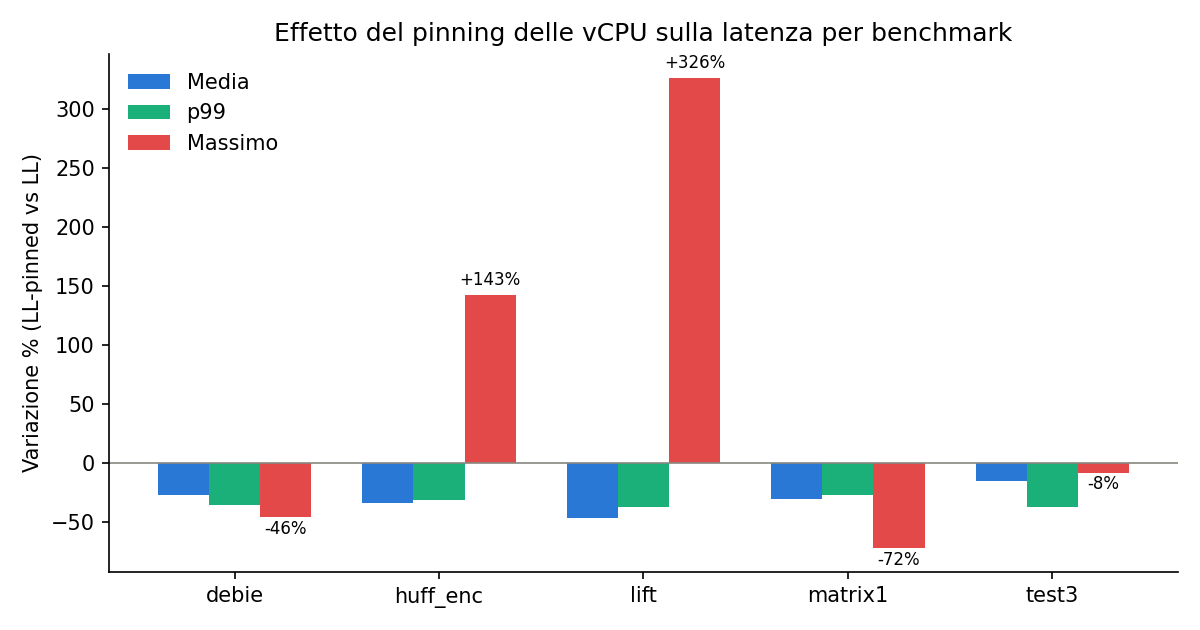
\includegraphics[width=\linewidth]{../Xen/tests_tacle_dom0_stress/plots/latency_delta_chart.png}
\caption{Effetto del pinning delle vCPU sulla latenza per benchmark}
\end{figure}

\emph{Percentage variation of the mean, p99, and maximum (LL-pinned vs
LL) for the five TACLe benchmarks: debie, huff\_enc, lift, matrix1,
test3.}

\paragraph{\% Variation LL-pinned vs
LL}\label{variation-ll-pinned-vs-ll}

\begin{table*}
\centering
\caption{Xen Variation LL-pinned vs.\ LL}
\label{tab:xen:ll-pinned-vs-ll}
\begin{tabularx}{\linewidth}{@{}YYYY@{}}
\toprule
\textbf{Benchmark} & \textbf{$\Delta Average$} & \textbf{$\Delta p99$} & \textbf{$\Delta Max$}\tabularnewline
\midrule
debie & -26.5\% & -35.8\% & -45.8\%\tabularnewline
huff\_enc & -34.1\% & -31.4\% & +142.6\%\tabularnewline
lift & -46.3\% & -37.0\% & +326.5\%\tabularnewline
matrix1 & -30.7\% & -26.6\% & -72.1\%\tabularnewline
test3 & -15.4\% & -37.2\% & -8.2\%\tabularnewline
\bottomrule
\end{tabularx}
\end{table*}

\paragraph{1- Pinning systematically improves typical
latency}\label{pinning-systematically-improves-typical-latency}

Across all five benchmarks, without exception, vCPU pinning reduces both
the mean latency (from -15\% to -46\%) and the p99 (from -27\% to
-37\%). This confirms the expected effect: fixing the DomU vCPUs to
dedicated physical cores eliminates the variability introduced by the
Dom0 scheduler and inter-core migrations, making the temporal behavior
more predictable in the typical case.

\paragraph{2- Tail anomaly: pinning worsening the worst
case}\label{tail-anomaly-pinning-worsening-the-worst-case}

On debie, matrix1, and test3, pinning also improves the worst-case
(lower maximum). But on lift and huff\_enc the opposite happens: the
maximum latency increases drastically (+326\% on lift, +143\% on
huff\_enc), and huff\_enc-pinned registers a histogram overflow, a sign
that at least one sample exceeded even the maximum expected bucket ---
the actual peak could therefore be even higher than reported.

This is the most significant result to document: pinning is not a
unilateral guarantee of improvement. It reduces variance in the common
case, but if the pinned core is not completely isolated from external
interruptions (housekeeping IRQs, Dom0 timers, one of the stressors),
when that rare interference occurs its impact is concentrated entirely
on a single dedicated core instead of being distributed, producing an
isolated spike much larger than what would happen with free scheduling.

\begin{figure}
\centering
\includesvg[width=\linewidth]{../Xen/tests_tacle_dom0_stress/plots/stressor_TACLe_debie_boxplot.svg}
\caption{TACLe benchmark - debie stress dom0}
\end{figure}

\begin{figure}
\centering
\includesvg[width=\linewidth]{../Xen/tests_tacle_dom0_stress/plots/stressor_TACLe_matrix1_boxplot.svg}
\caption{TACLe benchmark - matrix1 stress dom0}
\end{figure}

\begin{figure}
\centering
\includesvg[width=\linewidth]{../Xen/tests_tacle_dom0_stress/plots/stressor_TACLe_test3_boxplot.svg}
\caption{TACLe benchmark - test3 stress dom0}
\end{figure}

\paragraph{3- Consistency between scale and
behavior}\label{consistency-between-scale-and-behavior}

The order of magnitude of latency varies greatly between benchmarks
(from hundreds of nanoseconds for matrix1 to tens of milliseconds for
debie), reflecting the different computational complexity of the TACLe
workloads. The mean/p99 improvement pattern with pinning is maintained
regardless of the scale, which reinforces the idea that it is a
structural effect of pinning itself and not an artifact linked to the
duration of the single benchmark.

\begin{figure}
\centering
\includesvg[width=\linewidth]{../Xen/tests_tacle_dom0_stress/plots/stressor_TACLe_lift_boxplot.svg}
\caption{TACLe benchmark - lift stress dom0}
\end{figure}

\begin{figure}
\centering
\includesvg[width=\linewidth]{../Xen/tests_tacle_dom0_stress/plots/stressor_TACLe_huffenc_boxplot.svg}
\caption{TACLe benchmark - huff\_enc stress dom0}
\end{figure}

\subsection{PV AND PVH DOMUS}\label{pv-and-pvh-domus-1}

In their previous work, Abeni and Faggioli concluded that in Xen,
virtualization technology played a major role in scheduling latencies
due to a priority inversion bug in how the Device Model operated.
Specifically, they noted that the QEMU process acting as the DomU DM did
not execute with high priority, allowing it to be preempted by the
workload.

We previously attempted to reproduce this issue using a newer version of
Xen (4.17.3) but did not observe the same trend. We also tried assigning
maximum priority to the QEMU process in Dom0, which yielded no
noticeable improvement. Consequently, we concluded that this priority
inversion bug has been fixed for HVM DomUs.

To further verify this conclusion, we extended our analysis to PV and
PVH guests. In this section, we reproduce the most relevant scenarios
for guests running on these different virtualization technologies and
analyze their resulting behaviors.

\subsubsection{RT Kernel and
PARAVIRTUALIZATION}\label{rt-kernel-and-paravirtualization}

While configuring the PV guest, we encountered the same issue observed
during the \href{../Setup/README.md\#problems-with-preempt_rt}{initial
setup process}. This time, because the output logs were routed to the
terminal, we were able to identify the cause. The logs revealed a
\textbf{soft CPU lockup}, confirming that the issue stemmed from the
\texttt{PREEMPT\_RT} patch. We hypothesize that this failure relates to
how the patch modifies low-level mechanisms---such as replacing
spinlocks with mutexes---which introduces compatibility issues with
paravirtualization. This also explains why the \texttt{PREEMPT\_RT}
patch failed in Dom0, as it is inherently a PV guest. Additionally, we
attempted to configure Dom0 as a PVH guest; however, this setup resulted
in continuous automatic reboots. Without access to system logs or
graphical output to diagnose the root cause, we were unable to
troubleshoot the error and ultimately abandoned this configuration.
Consequently, for the subsequent tests, we replaced the RT kernel with
the Low-Latency kernel in the DomU as well.

\begin{figure}
\centering
\includesvg[width=\linewidth]{../Xen/tests_pv_pvh/plots/svg/xen_guesttypecompare_nonoise.svg}
\caption{Comparing HVM, PV and PVH guests - Credit2 Scheduler (No
Noise)}
\end{figure}

\subsubsection{LOW LATENCY DOM0 AND LOW LATENCY DOMU (PV
DomU)}\label{low-latency-dom0-and-low-latency-domu-pv-domu}

This section analyzes the results obtained from a 5-minute execution of
the \texttt{cyclictest} utility within a Xen virtualized environment,
explicitly assessing a Paravirtualized (PV) guest. The configuration
features a ``Low Latency'' kernel deployed on both the privileged domain
(Dom0) and the unprivileged user domain (DomU). This test evaluates the
baseline performance of the dynamic scheduler without static vCPU
pinning and without any artificial stress workload applied to Dom0.

\paragraph{Nominal Performance and Average
Latency}\label{nominal-performance-and-average-latency-23}

The data obtained from the \texttt{cyclictest} execution reveals the
baseline virtualization overhead and scheduling behavior in an
undisturbed, unpinned PV configuration. The average latency recorded
during the test was 37 $\mu s$, significantly higher than any other baseline
average latency we recorded. The absolute minimum latency achieved was 4
$\mu s$.

\paragraph{Worst-Case Execution Time (WCET)
Analysis}\label{worst-case-execution-time-wcet-analysis-25}

The analysis of the Worst-Case Execution Time (WCET) provides insight
into the system's baseline ability to bound execution delays. Over the
duration of the test, the absolute maximum latency recorded was 525 $\mu s$.

\paragraph{Observations on the Baseline PV Unpinned
Environment}\label{observations-on-the-baseline-pv-unpinned-environment}

The empirical data collected from this test yields the following
observations regarding the behavior of the Low Latency PV DomU running
on a Low Latency Dom0 without vCPU pinning in a quiet environment:

\begin{itemize}
\item
  \textbf{Bounded WCET:} The maximum latency was contained at 525 $\mu s$.
\item
  \textbf{Baseline Jitter:} The average latency of 37 $\mu s$ confirms the
  presence of scheduling jitter.
\end{itemize}

\subsubsection{LOW LATENCY DOM0 AND REAL-TIME DOMU (PVH
DomU)}\label{low-latency-dom0-and-real-time-domu-pvh-domu}

This section analyzes the results obtained from a 5-minute execution of
the \texttt{cyclictest} utility within a Xen virtualized environment,
explicitly assessing a PVH guest. The configuration features a ``Low
Latency'' kernel deployed on the privileged domain (Dom0) and a
Real-Time (\texttt{PREEMPT\_RT}) kernel on the unprivileged user domain
(DomU). This test evaluates the baseline performance of the dynamic
Credit2 scheduler without static vCPU pinning and without any artificial
stress workload applied to Dom0.

\paragraph{Nominal Performance and Average
Latency}\label{nominal-performance-and-average-latency-24}

The data obtained from the \texttt{cyclictest} execution reveals the
baseline virtualization overhead and scheduling behavior in an
undisturbed, unpinned configuration. The average latency recorded during
the test was 32 $\mu s$. The absolute minimum latency achieved was 3 $\mu s$. The
histogram data indicates a broad distribution of execution latencies,
demonstrating the variability introduced by dynamic scheduling even in
the absence of host-level contention.

\paragraph{Worst-Case Execution Time (WCET)
Analysis}\label{worst-case-execution-time-wcet-analysis-26}

The analysis of the Worst-Case Execution Time (WCET) provides insight
into the system's baseline ability to bound execution delays. Over the
duration of the test, the absolute maximum latency recorded was 76 $\mu s$.
The system successfully avoided any histogram overflows.

\paragraph{Observations on the Baseline PVH Unpinned
Environment}\label{observations-on-the-baseline-pvh-unpinned-environment}

The empirical data collected from this test yields the following
observations regarding the behavior of the RT PVH DomU running on a Low
Latency Dom0 without vCPU pinning in a quiet environment:

\begin{itemize}
\item
  \textbf{Bounded WCET:} The maximum latency was contained at 76 $\mu s$,
  indicating that the combination of the RT guest kernel and the Low
  Latency host kernel provides a stable upper bound when the host is not
  under load.
\item
  \textbf{Baseline Jitter:} The average latency of 32 $\mu s$ and the wide
  spread of nominal execution times confirm the presence of significant
  scheduling jitter. This variability highlights the inherent impact of
  the dynamic Credit2 hypervisor scheduler, even without resource
  contention from a \texttt{stressdom0} workload.
\end{itemize}

\begin{figure}
\centering
\includesvg[width=\linewidth]{../Xen/tests/plots/svg/Comparing_HVM_PV_PVH_credit2_boxplot.svg}
\caption{Comparing HVM, PV and PVH guests - Credit2 Scheduler (No
Noise)}
\end{figure}

\subsection{IMPACT OF THE STRESS WORKLOAD ON DIFFERENT VIRTUALIZATION
TECHNOLOGIES}\label{impact-of-the-stress-workload-on-different-virtualization-technologies}

To assess the influence of the underlying virtualization architecture on
system determinism, this phase of testing introduces a background stress
workload in the privileged domain (Dom0) while executing the
\texttt{cyclictest} probe within PV and PVH guests. Building upon our
earlier findings---which demonstrated that modern Hardware Virtual
Machine (HVM) configurations successfully manage latency bounds without
suffering from historical QEMU-induced preemption anomalies---this
evaluation aims to compare how alternative virtualization models respond
to resource contention. Ultimately, the analysis highlights that while
PVH and HVM achieve highly similar performance levels, the PV
architecture exhibits the worst performance among all three
technologies.

Experimental analysis reveals that moving away from full hardware
virtualization fundamentally alters the system dynamics, highlighting
key architectural trade-offs when employing PV and PVH configurations:

\begin{itemize}
\item
  \textbf{Absence of the Device Model:} Unlike HVM guests, PV and PVH
  architectures do not rely on a QEMU instance running in Dom0 for
  hardware emulation. While our previous tests confirmed that modern Xen
  deployments resolve the historical priority inversion bugs associated
  with QEMU, evaluating PV and PVH guests allows us to observe system
  behavior completely isolated from Device Model interactions.
\item
  \textbf{Constraints on Kernel Optimization:} While paravirtualization
  removes the Device Model variable, it introduces strict constraints
  regarding real-time optimizations. As established during the initial
  setup, the inherent incompatibility of the \texttt{PREEMPT\_RT} patch
  with PV guests necessitated a fallback to a Low Latency kernel. This
  dynamic fundamentally shifts the performance bottleneck from
  hypervisor-level interference to guest-level scheduling limitations,
  severely penalizing the PV configuration.
\item
  \textbf{Comparative Resilience to Contention:} Evaluating these
  paravirtualized environments under Dom0 stress provides a direct
  contrast to the HVM data. The empirical results reveal that the
  intrinsically lighter virtualization footprint of the PV architecture
  cannot compensate for the lack of rigorous, real-time guest
  optimizations, resulting in the poorest latency bounds. Conversely,
  the PVH architecture overcomes these limitations, demonstrating a
  resilience to contention and overall performance metrics that are
  remarkably similar to those of HVM.
\end{itemize}

In this section, we present a detailed comparative analysis of these
configurations, quantifying the execution latencies of PV and PVH guests
under stress to determine their overall viability for predictable,
latency-sensitive applications compared to their HVM counterparts.

\begin{figure}
\centering
\includesvg[width=\linewidth]{../Xen/tests_pv_pvh/plots/svg/xen_guesttypecompare_backgroundnoise.svg}
\caption{Comparing HVM, PV and PVH guests - Credit2 Scheduler
(Background Noise)}
\end{figure}

\subsubsection{LOW LATENCY DOM0 AND LOW LATENCY DOMU (PV
DomU)}\label{low-latency-dom0-and-low-latency-domu-pv-domu-1}

This section details the analysis of a 5-minute execution of the
\texttt{cyclictest} utility within a Xen virtualized environment,
specifically evaluating a Paravirtualized (PV) guest. This configuration
features a ``Low Latency'' kernel deployed on both the privileged domain
(Dom0) and the unprivileged user domain (DomU). Crucially, this test was
conducted without static vCPU pinning and while Dom0 was subjected to a
significant background stress workload (\texttt{stressdom0}). The
objective is to evaluate the latency characteristics and the impact of
host-level contention when both domains utilize low-latency
optimizations in an unpinned PV environment.

\paragraph{Nominal Performance and Average
Latency}\label{nominal-performance-and-average-latency-25}

The data obtained from the \texttt{cyclictest} execution reveals the
baseline virtualization overhead and scheduling jitter under stress
conditions. The average latency recorded during the test was 40 $\mu s$. The
absolute minimum latency achieved was 4 $\mu s$. The histogram data indicates
a broad distribution of execution latencies, demonstrating the
variability introduced by the dynamic Credit2 scheduler when managing
host-level contention without vCPU pinning.

\paragraph{Worst-Case Execution Time (WCET)
Analysis}\label{worst-case-execution-time-wcet-analysis-27}

The analysis of the Worst-Case Execution Time (WCET) provides insight
into the system's ability to bound execution delays under stress. Over
the duration of the test, the absolute maximum latency recorded was 312
$\mu s$.

\paragraph{Observations on the Stressed PV Unpinned
Environment}\label{observations-on-the-stressed-pv-unpinned-environment}

The empirical data collected from this sustained test yields the
following observations regarding the behavior of the Low Latency PV DomU
running on a Low Latency Dom0 without vCPU pinning under
\texttt{stressdom0}:

\begin{itemize}
\item
  \textbf{Bounded WCET:} The maximum latency was contained at 312 $\mu s$,
  indicating that the dual Low-Latency kernel setup provides a degree of
  stability under stress, preventing extreme multi-millisecond spikes
  despite the lack of pinning.
\item
  \textbf{Stress-Induced Jitter:} The average latency of 40 $\mu s$ and the
  wide spread of nominal execution times confirm the presence of
  significant scheduling jitter. This highlights the impact of dynamic
  hypervisor scheduling and resource contention from the
  \texttt{stressdom0} workload on a PV guest.
\end{itemize}

\subsubsection{LOW LATENCY DOM0 AND REAL-TIME DOMU (PVH
DomU)}\label{low-latency-dom0-and-real-time-domu-pvh-domu-1}

This section details the analysis of a 5-minute execution of the
\texttt{cyclictest} utility within a Xen virtualized environment,
explicitly assessing a PVH guest. The configuration features a ``Low
Latency'' kernel deployed on the privileged domain (Dom0) and a
Real-Time (\texttt{PREEMPT\_RT}) kernel on the unprivileged user domain
(DomU). Crucially, this test was conducted without static vCPU pinning
and while Dom0 was subjected to a significant background stress
workload. The objective is to evaluate the latency characteristics and
virtualization overhead introduced by the hypervisor when managing a PVH
guest under these specific, unpinned stress conditions.

\paragraph{Nominal Performance and Average
Latency}\label{nominal-performance-and-average-latency-26}

The data obtained from the \texttt{cyclictest} execution reveals the
baseline virtualization overhead and scheduling jitter inherent in this
unpinned configuration. The average latency recorded during the test was
35 $\mu s$. The absolute minimum latency achieved was 3 $\mu s$. The histogram
data indicates a broad distribution of execution latencies,
demonstrating the variability introduced when dynamic scheduling is
utilized under host-level contention.

\paragraph{Worst-Case Execution Time (WCET)
Analysis}\label{worst-case-execution-time-wcet-analysis-28}

The analysis of the Worst-Case Execution Time (WCET) provides insight
into the system's ability to bound execution delays under stress. Over
the duration of the test, the absolute maximum latency recorded was 157
$\mu s$.

\paragraph{Observations on the PVH Unpinned
Environment}\label{observations-on-the-pvh-unpinned-environment}

The empirical data collected from this sustained test yields the
following observations regarding the behavior of the RT PVH DomU running
on a Low Latency Dom0 without vCPU pinning:

\begin{itemize}
\item
  \textbf{Bounded WCET:} The maximum latency was contained at 157 $\mu s$,
  indicating that the combination of the RT guest kernel and the Low
  Latency host kernel provided a degree of stability, preventing the
  extreme, multi-millisecond spikes that can occur in less optimized
  configurations.
\item
  \textbf{Hypervisor-Induced Jitter:} The average latency of 35 $\mu s$ and
  the wide spread of nominal execution times confirm the presence of
  significant scheduling jitter. This variability highlights the impact
  of dynamic hypervisor scheduling and resource contention from the
  \texttt{stressdom0} workload when vCPUs are not statically pinned to
  dedicated physical cores.
\end{itemize}

\begin{figure}
\centering
\includesvg[width=\linewidth]{../Xen/tests/plots/svg/Comparing_HVM_PV_PVH_stressdom0_credit2_boxplot.svg}
\caption{Comparing HVM, PV and PVH guests - Credit2 Scheduler
(Background Noise)}
\end{figure}

\subsection{COMPARATIVE ANALYSIS OF PV AND PVH ARCHITECTURES UNDER
STATIC
ALLOCATION}\label{comparative-analysis-of-pv-and-pvh-architectures-under-static-allocation}

Following the initial investigations into dynamic scheduling behavior,
this section presents a targeted comparative analysis of execution
latencies between Paravirtualized (PV) and Hardware Virtual Machine with
PV drivers (PVH) configurations. To eliminate the jitter introduced by
complex fair-share algorithms and evaluate the highest degree of
determinism achievable, these tests employ strict vCPU-to-pCPU pinning
across both the privileged domain (Dom0) and the unprivileged user
domain (DomU), effectively emulating the deterministic behavior of an
offline NULL scheduler.

The evaluation is conducted under ideal, unstressed conditions,
isolating the system from external background workloads. By analyzing
both PV and PVH DomU architectures in a quiet environment, we establish
a clean baseline for the inherent virtualization overhead that persists
even when static hardware allocation is employed.

This comparative approach aims to quantify the efficacy of strict
hardware isolation in bounding the Worst-Case Execution Time (WCET). By
observing the system's baseline predictability, the analysis highlights
the specific architectural nuances between PV and PVH environments,
demonstrating how effectively vCPU pinning manages nominal execution
latencies prior to the introduction of external stress factors.

\begin{figure}
\centering
\includesvg[width=\linewidth]{../Xen/tests_pv_pvh/plots/svg/xen_guesttypecompare_null_nonoise.svg}
\caption{Comparing HVM, PV and PVH guests - Null Scheduler (No Noise)}
\end{figure}

\subsubsection{LOW LATENCY DOM0 AND LOW LATENCY DOMU (PV
DomU)}\label{low-latency-dom0-and-low-latency-domu-pv-domu-2}

This section details the analysis of a 5-minute execution of the
\texttt{cyclictest} utility within a Xen virtualized environment,
specifically evaluating a Paravirtualized (PV) guest. The configuration
utilizes a ``Low Latency'' kernel for both the privileged domain (Dom0)
and the unprivileged user domain (DomU). Crucially, this test evaluates
the system emulating the static NULL scheduler with explicit vCPU
pinning, and it is conducted in a quiet environment without any
background \texttt{stressdom0} workload. The objective is to assess the
baseline latency and determinism of a PV guest when fully optimized
through static hardware allocation.

\paragraph{Nominal Performance and Average
Latency}\label{nominal-performance-and-average-latency-27}

The data obtained from the \texttt{cyclictest} execution reveals the
baseline virtualization overhead in this optimized, pinned PV
configuration. The average latency recorded during the test was 39 $\mu s$.
The absolute minimum latency achieved was 5 $\mu s$. While pinning isolates
the workload, the histogram indicates a spread in nominal execution
times, confirming that baseline virtualization jitter persists even with
a static scheduler.

\paragraph{Worst-Case Execution Time (WCET)
Analysis}\label{worst-case-execution-time-wcet-analysis-29}

The analysis of the Worst-Case Execution Time (WCET) highlights the
system's ability to bound execution delays under ideal, unstressed
conditions. Over the duration of the test, the absolute maximum latency
recorded was 492 $\mu s$.

\paragraph{Observations on the Baseline PV Pinned Environment (NULL
Scheduler)}\label{observations-on-the-baseline-pv-pinned-environment-null-scheduler}

The empirical data collected from this sustained test yields the
following observations regarding the behavior of the Low Latency PV DomU
running on a Low Latency Dom0 with static pinning using the NULL
scheduler:

\begin{itemize}
\item
  \textbf{Bounded WCET:} The maximum latency was contained at 492 $\mu s$.
  While higher than fully patched RT configurations, this demonstrates a
  stable upper bound for a PV guest utilizing Low Latency kernels in a
  pinned environment.
\item
  \textbf{Baseline Jitter:} The average latency of 39 $\mu s$ indicates that
  the static allocation provided by the NULL scheduler does not
  completely eliminate the inherent scheduling jitter associated with
  the virtualization layer itself.
\end{itemize}

\subsubsection{LOW LATENCY DOM0 AND REAL TIME DOMU (PVH
DomU)}\label{low-latency-dom0-and-real-time-domu-pvh-domu-2}

This section details the analysis of a 5-minute execution of the
\texttt{cyclictest} utility within a Xen virtualized environment,
specifically evaluating a PVH guest. The configuration utilizes a ``Low
Latency'' kernel deployed on the privileged domain (Dom0) and a
Real-Time (\texttt{PREEMPT\_RT}) kernel on the unprivileged user domain
(DomU). This test evaluates the system emulating the static NULL
scheduler with explicit vCPU pinning, and it is conducted in a quiet
environment without any background stress workload. The objective is to
assess the baseline latency and determinism of a highly optimized PVH
guest when fully isolated through static hardware allocation.

\paragraph{Nominal Performance and Average
Latency}\label{nominal-performance-and-average-latency-28}

The data obtained from the \texttt{cyclictest} execution reveals the
baseline virtualization overhead in this optimized, pinned PVH
configuration. The average latency recorded during the test was 33 $\mu s$.
The absolute minimum latency achieved was 3 $\mu s$. The histogram indicates
a tight distribution of nominal execution times, confirming that pinning
effectively shields the guest and provides high consistency.

\paragraph{Worst-Case Execution Time (WCET)
Analysis}\label{worst-case-execution-time-wcet-analysis-30}

The analysis of the Worst-Case Execution Time (WCET) highlights the
system's ability to rigidly bound execution delays under ideal,
unstressed conditions. Over the duration of the test, the absolute
maximum latency recorded was 71 $\mu s$.

\paragraph{Observations on the Baseline PVH Pinned Environment (NULL
Scheduler)}\label{observations-on-the-baseline-pvh-pinned-environment-null-scheduler}

The empirical data collected from this sustained test yields the
following observations regarding the behavior of the RT PVH DomU running
on a Low Latency Dom0 with static pinning using the NULL scheduler:

\begin{itemize}
\item
  \textbf{Strictly Bounded WCET:} The maximum latency was contained at
  71 $\mu s$. This demonstrates an exceptionally stable upper bound for a PVH
  guest, proving that the combination of RT guest kernels, Low Latency
  host kernels, vCPU pinning, and the NULL scheduler provides hard
  real-time characteristics.
\item
  \textbf{Baseline Jitter:} The average latency of 33 $\mu s$ and the tight
  spread of execution times indicate a high level of consistency in the
  static allocation provided by the NULL scheduler.
\end{itemize}

\begin{figure}
\centering
\includesvg[width=\linewidth]{../Xen/tests/plots/svg/Comparing_HVM_PV_PVH_null_boxplot.svg}
\caption{Comparing HVM, PV and PVH guests - Null Scheduler (No Noise)}
\end{figure}

\subsection{IMPACT OF THE STRESS WORKLOAD ON PV AND PVH ARCHITECTURES
UNDER STATIC
ALLOCATION}\label{impact-of-the-stress-workload-on-pv-and-pvh-architectures-under-static-allocation}

Building upon the baseline established in the ideal, unstressed
environment, this phase introduces a severe background stress workload
(\texttt{stressdom0}) into the privileged control domain. The primary
objective is to evaluate the resilience of static vCPU pinning---acting
as a surrogate for the offline NULL scheduler---when the host system is
heavily saturated with competing processes.

By subjecting both the Paravirtualized (PV) and Hardware Virtual Machine
with PV drivers (PVH) guests to this intense host-level contention, we
can determine whether strict hardware isolation alone is sufficient to
prevent latency spikes from degrading guest determinism. This evaluation
specifically tests the boundaries of system predictability, observing
the extent to which stress-induced jitter manages to bypass the static
allocation and affect the isolated virtual CPUs.

The subsequent analyses reveal a distinct divergence in architectural
resilience under load. While vCPU pinning provides a foundational level
of stability for both configurations, the empirical data highlights that
the PV architecture remains susceptible to measurable interference from
the host. Conversely, the PVH architecture demonstrates exceptional
isolation, successfully shielding its critical execution paths and
maintaining rigid Worst-Case Execution Time (WCET) boundaries despite
the intense resource contention within Dom0.

\begin{figure}
\centering
\includesvg[width=\linewidth]{../Xen/tests_pv_pvh/plots/svg/xen_guesttypecompare_null_backgroundnoise.svg}
\caption{Comparing HVM, PV and PVH guests - Null Scheduler (Background
Noise)}
\end{figure}

\subsubsection{LOW LATENCY DOM0 AND LOW LATENCY DOMU (PV
DomU)}\label{low-latency-dom0-and-low-latency-domu-pv-domu-3}

This section analyzes the results obtained from a 5-minute execution of
the \texttt{cyclictest} utility within a Xen virtualized environment,
explicitly assessing a Paravirtualized (PV) guest. The configuration
features a ``Low Latency'' kernel deployed on both the privileged domain
(Dom0) and the unprivileged user domain (DomU). Crucially, this test
evaluates the performance of the NULL scheduler with explicit vCPU
pinning while Dom0 is subjected to a significant background stress
workload (\texttt{stressdom0}). The objective is to evaluate the latency
characteristics and the ability of the NULL scheduler's static
allocation to manage host-level contention in an optimized, pinned PV
environment.

\paragraph{Nominal Performance and Average
Latency}\label{nominal-performance-and-average-latency-29}

The data obtained from the \texttt{cyclictest} execution reveals the
baseline virtualization overhead and scheduling behavior under stress
conditions when utilizing the static NULL scheduler with pinning. The
average latency recorded during the test was 39 $\mu s$. The absolute minimum
latency achieved was 4 $\mu s$. The histogram data indicates a broad
distribution of execution latencies, demonstrating the variability
introduced by the \texttt{stressdom0} workload, even when a static,
pinned scheduler is employed.

\paragraph{Worst-Case Execution Time (WCET)
Analysis}\label{worst-case-execution-time-wcet-analysis-31}

The analysis of the Worst-Case Execution Time (WCET) provides insight
into the system's ability to bound execution delays under stress. Over
the duration of the test, the absolute maximum latency recorded was 285
$\mu s$.

\paragraph{Observations on the Stressed PV Pinned Environment (NULL
Scheduler)}\label{observations-on-the-stressed-pv-pinned-environment-null-scheduler}

The empirical data collected from this sustained test yields the
following observations regarding the behavior of the Low Latency PV DomU
running on a Low Latency Dom0 with vCPU pinning under
\texttt{stressdom0} using the NULL scheduler:

\begin{itemize}
\item
  \textbf{Bounded WCET:} The maximum latency was contained at 285 $\mu s$.
  This indicates that the combination of the dual Low-Latency kernel
  setup and the pinned NULL scheduler provides a degree of stability
  under stress, establishing a tighter bound than unpinned
  configurations.
\item
  \textbf{Stress-Induced Jitter:} The average latency of 39 $\mu s$ and the
  wide spread of nominal execution times confirm the presence of
  significant scheduling jitter. This highlights that even with a
  statically pinned scheduler, resource contention from the
  \texttt{stressdom0} workload on a PV guest still significantly impacts
  latency stability.
\end{itemize}

\subsubsection{LOW LATENCY DOM0 AND REAL-TIME DOMU (PVH
DomU)}\label{low-latency-dom0-and-real-time-domu-pvh-domu-3}

This section analyzes the results obtained from a 5-minute execution of
the \texttt{cyclictest} utility within a Xen virtualized environment,
evaluating a Hardware Virtual Machine with Paravirtualized drivers (PVH)
guest. The configuration features a ``Low Latency'' kernel deployed on
the privileged domain (Dom0) and a Real-Time (\texttt{PREEMPT\_RT})
kernel on the unprivileged user domain (DomU). Crucially, this test
evaluates the performance of the NULL scheduler with explicit vCPU
pinning while Dom0 is subjected to a background stress workload
(\texttt{stressdom0}). The objective is to evaluate the latency
characteristics and the ability of the NULL scheduler's static
allocation to maintain determinism under host-level contention in an
optimized, pinned PVH environment.

\paragraph{Nominal Performance and Average
Latency}\label{nominal-performance-and-average-latency-30}

The data obtained from the \texttt{cyclictest} execution reveals the
baseline virtualization overhead and scheduling behavior under stress
conditions when utilizing the static NULL scheduler with vCPU pinning.
The average latency recorded during the test was 33 $\mu s$. The absolute
minimum latency achieved was 3 $\mu s$. The data indicates a concentrated
distribution of nominal execution times, demonstrating a high level of
consistency despite the background load.

\paragraph{Worst-Case Execution Time (WCET)
Analysis}\label{worst-case-execution-time-wcet-analysis-32}

The analysis of the Worst-Case Execution Time (WCET) provides insight
into the system's ability to rigidly bound execution delays under
stress. Over the duration of the test, the absolute maximum latency
recorded was strictly capped at 71 $\mu s$.

\paragraph{Observations on the Stressed PVH Pinned Environment (NULL
Scheduler)}\label{observations-on-the-stressed-pvh-pinned-environment-null-scheduler}

The empirical data collected from this sustained test yields the
following observations regarding the behavior of the RT PVH DomU running
on a Low Latency Dom0 with vCPU pinning under \texttt{stressdom0} using
the NULL scheduler:

\begin{itemize}
\item
  \textbf{Strictly Bounded WCET:} The maximum latency was contained at
  71 $\mu s$. This demonstrates that the combination of the
  \texttt{PREEMPT\_RT} guest kernel, the Low-Latency host kernel, static
  vCPU pinning, and the NULL scheduler provides exceptional stability
  and successfully shields the critical guest execution path from severe
  preemption spikes.
\item
  \textbf{Resilience to Host Stress:} The average latency of 33 $\mu s$ and
  the rigid WCET boundary confirm that this highly optimized, static PVH
  configuration effectively mitigates the severe scheduling jitter
  typically induced by host-level resource contention.
\end{itemize}

\begin{figure}
\centering
\includesvg[width=\linewidth]{../Xen/tests/plots/svg/Comparing_HVM_PV_PVH_stressdom0_null_boxplot.svg}
\caption{Comparing HVM, PV and PVH guests - Null Scheduler (Background
Noise)}
\end{figure}

\subsection{SUMMARY OF RESULTS (PV AND
PVH)}\label{summary-of-results-pv-and-pvh}

To synthesize the findings from our latency evaluations, the following
table aggregates the Worst-Case Execution Time (WCET) results recorded
across the three evaluated Xen virtualization modes: Hardware Virtual
Machine (HVM), Hardware Virtual Machine with Paravirtualized drivers
(PVH), and fully Paravirtualized (PV) guests.

\begin{table*}
\centering
\caption{Xen Virtualization Modes WCET Comparison}
\label{tab:xen:wcet-comparison}
\begin{tabularx}{\linewidth}{@{}YYYY@{}}
\toprule
Configuration & HVM & PVH & PV\tabularnewline
\midrule
\textbf{BASELINE} & 71 & 76 & 525\tabularnewline
\textbf{STRESS WORKLOAD} & 209 & 157 & 312\tabularnewline
\textbf{vCPU PINNING BASELINE} & 65 & 71 & 492\tabularnewline
\textbf{vCPU PINNING STRESS WORKLOAD} & 163 & 71 & 285\tabularnewline
\bottomrule
\end{tabularx}
\end{table*}

This section provides a quantitative breakdown of the percentage
increments for both the average latency (Mean ± Standard Deviation) and
the maximum latency (WCET) across Xen's three virtualization modes: HVM,
PV, and PVH. The analysis evaluates the performance degradation caused
by a heavy stress workload introduced in the control domain (Dom0).

The following tables illustrate the system's behavior under the default
dynamic scheduler. These results highlight the performance impact of the
Dom0 stress workload when no hardware isolation mechanisms are applied.
\#\#\# HVM LL RT

\begin{table*}
\centering
\caption{HVM Latency Statistics}
\begin{tabularx}{\linewidth}{@{}YYY@{}}
\toprule
METRIC & BASELINE & STRESS WORKLOAD\tabularnewline
\midrule
\textbf{Average ± SD} & 32.89 ± 15.14 $\mu s$ & 35.66 ± 15.60 $\mu s$\tabularnewline
\textbf{WCET (Max)} & 71 $\mu s$ & 209 $\mu s$\tabularnewline
\bottomrule
\end{tabularx}
\end{table*}

\textbf{PERCENTAGE INCREMENTS (Stress vs.~Baseline):} * Average
Increment: +8.42\% * WCET Increment: +194.37\%

\subsubsection{PV LL-LL}\label{pv-ll-ll}

\begin{table*}
\centering
\caption{PV Latency Statistics}
\begin{tabularx}{\linewidth}{@{}YYY@{}}
\toprule
METRIC & BASELINE & STRESS WORKLOAD\tabularnewline
\midrule
\textbf{Average ± SD} & 37.17 ± 14.69 $\mu s$ & 40.20 ± 16.22 $\mu s$\tabularnewline
\textbf{WCET (Max)} & 525 $\mu s$ & 312 $\mu s$\tabularnewline
\bottomrule
\end{tabularx}
\end{table*}

\textbf{PERCENTAGE INCREMENTS (Stress vs.~Baseline):} * Average
Increment: +8.16\% * WCET Increment: -40.57\%

\subsubsection{PVH LL-RT}\label{pvh-ll-rt}

\begin{table*}
\centering
\caption{PVH Latency Statistics}
\begin{tabularx}{\linewidth}{@{}YYY@{}}
\toprule
METRIC & BASELINE & STRESS WORKLOAD\tabularnewline
\midrule
\textbf{Average ± SD} & 32.40 ± 15.36 $\mu s$ & 35.58 ± 15.50 $\mu s$\tabularnewline
\textbf{WCET (Max)} & 76 $\mu s$ & 157 $\mu s$\tabularnewline
\bottomrule
\end{tabularx}
\end{table*}

\textbf{PERCENTAGE INCREMENTS (Stress vs.~Baseline):} * Average
Increment: +9.82\% * WCET Increment: +106.58\%


The tables below evaluate the resilience of the same configurations when
strict vCPU pinning is enforced. By isolating Dom0 and DomU on dedicated
physical cores, this scenario demonstrates how static hardware
allocation mitigates scheduling interference under stress.

\subsubsection{HVM LL RT}\label{hvm-ll-rt}

\begin{table*}
\centering
\caption{HVM Latency Statistics - vCPU Pinning}
\begin{tabularx}{\linewidth}{@{}YYY@{}}
\toprule
METRIC & vCPU PINNING BASELINE & vCPU PINNING STRESS WORKLOAD\tabularnewline
\midrule
\textbf{Average ± SD} & 33.09 ± 15.18 $\mu s$ & 32.73 ± 15.09 $\mu s$\tabularnewline
\textbf{WCET (Max)} & 65 $\mu s$ & 163 $\mu s$\tabularnewline
\bottomrule
\end{tabularx}
\end{table*}

\textbf{PERCENTAGE INCREMENTS (Stress vs.~Baseline):} * Average
Increment: -1.11\% * WCET Increment: +150.77\%

\subsubsection{PV LL-LL (Static vCPU
Pinning)}\label{pv-ll-ll-static-vcpu-pinning}

\begin{table*}
\centering
\caption{PV Latency Statistics - vCPU Pinning}
\begin{tabularx}{\linewidth}{@{}YYY@{}}
\toprule
METRIC & vCPU PINNING BASELINE & vCPU PINNING STRESS WORKLOAD\tabularnewline
\midrule
\textbf{Average ± SD} & 40.00 ± 14.71 $\mu s$ & 39.15 ± 15.23 $\mu s$\tabularnewline
\textbf{WCET (Max)} & 492 $\mu s$ & 285 $\mu s$\tabularnewline
\bottomrule
\end{tabularx}
\end{table*}

\textbf{PERCENTAGE INCREMENTS (Stress vs.~Baseline):} * Average
Increment: -2.13\% * WCET Increment: -42.07\%

\subsubsection{PVH LL-RT (Static vCPU
Pinning)}\label{pvh-ll-rt-static-vcpu-pinning}

\begin{table*}
\centering
\caption{PVH Latency Statistics - vCPU Pinning}
\begin{tabularx}{\linewidth}{@{}YYY@{}}
\toprule
METRIC & vCPU PINNING BASELINE & vCPU PINNING STRESS WORKLOAD\tabularnewline
\midrule
\textbf{Average ± SD} & 33.16 ± 15.12 $\mu s$ & 33.20 ± 15.09 $\mu s$\tabularnewline
\textbf{WCET (Max)} & 71 $\mu s$ & 71 $\mu s$\tabularnewline
\bottomrule
\end{tabularx}
\end{table*}

\textbf{PERCENTAGE INCREMENTS (Stress vs.~Baseline):} * Average
Increment: +0.14\% * WCET Increment: 0.00\%


\section{Conclusion}
\label{sec:conclusion}
This paper presented a systematic experimental characterization of Xen and KVM
as real-time hypervisors for mixed-criticality workloads.
Across all tested configurations, achieving bounded worst-case latencies requires
an \emph{end-to-end} real-time approach: a \texttt{PREEMPT\_RT}-patched kernel
is necessary at both host and guest level, and vCPU pinning is essential for
shielding time-critical domains from background interference.

For KVM, the combination of an RT host kernel, an RT guest kernel, and vCPU
pinning consistently reduces worst-case latency; however, multi-millisecond
spikes under heavy stress workloads remain a concern.
For Xen, the PVH guest type with the Null scheduler and strict vCPU pinning
delivers the tightest latency bounds.
TACLe benchmark results confirm that lightweight tasks (e.g., \texttt{matrix1},
\texttt{huff\_enc}) maintain near-deterministic execution, while heavy workloads
(e.g., DEBIE, \texttt{test3}) remain sensitive to scheduling noise across all
configurations.
Future work will investigate memory-bandwidth partitioning via Intel~RDT and
the integration of Unikraft~\cite{kuenzer2021} unikernels as latency-aware
guest alternatives.


\section*{Acknowledgment}
The authors wish to thank Ch.mo Prof.\ Marcello~Cinque, Ch.moProf.\ Luigi~De~Simone,
and Ing.\ Francesco~Boccola of the University of Naples ``Federico~II''
for their guidance and support throughout this project.


% References
\bibliography{bibliography}
\bibliographystyle{IEEEtran}


\end{document}
